\documentclass[]{book}
\usepackage{lmodern}
\usepackage{amssymb,amsmath}
\usepackage{ifxetex,ifluatex}
\usepackage{fixltx2e} % provides \textsubscript
\ifnum 0\ifxetex 1\fi\ifluatex 1\fi=0 % if pdftex
  \usepackage[T1]{fontenc}
  \usepackage[utf8]{inputenc}
\else % if luatex or xelatex
  \ifxetex
    \usepackage{mathspec}
  \else
    \usepackage{fontspec}
  \fi
  \defaultfontfeatures{Ligatures=TeX,Scale=MatchLowercase}
\fi
% use upquote if available, for straight quotes in verbatim environments
\IfFileExists{upquote.sty}{\usepackage{upquote}}{}
% use microtype if available
\IfFileExists{microtype.sty}{%
\usepackage{microtype}
\UseMicrotypeSet[protrusion]{basicmath} % disable protrusion for tt fonts
}{}
\usepackage[margin=1in]{geometry}
\usepackage{hyperref}
\hypersetup{unicode=true,
            pdftitle={plotly for R},
            pdfauthor={Carson Sievert},
            pdfborder={0 0 0},
            breaklinks=true}
\urlstyle{same}  % don't use monospace font for urls
\usepackage{natbib}
\bibliographystyle{apalike}
\usepackage{color}
\usepackage{fancyvrb}
\newcommand{\VerbBar}{|}
\newcommand{\VERB}{\Verb[commandchars=\\\{\}]}
\DefineVerbatimEnvironment{Highlighting}{Verbatim}{commandchars=\\\{\}}
% Add ',fontsize=\small' for more characters per line
\usepackage{framed}
\definecolor{shadecolor}{RGB}{248,248,248}
\newenvironment{Shaded}{\begin{snugshade}}{\end{snugshade}}
\newcommand{\KeywordTok}[1]{\textcolor[rgb]{0.13,0.29,0.53}{\textbf{{#1}}}}
\newcommand{\DataTypeTok}[1]{\textcolor[rgb]{0.13,0.29,0.53}{{#1}}}
\newcommand{\DecValTok}[1]{\textcolor[rgb]{0.00,0.00,0.81}{{#1}}}
\newcommand{\BaseNTok}[1]{\textcolor[rgb]{0.00,0.00,0.81}{{#1}}}
\newcommand{\FloatTok}[1]{\textcolor[rgb]{0.00,0.00,0.81}{{#1}}}
\newcommand{\ConstantTok}[1]{\textcolor[rgb]{0.00,0.00,0.00}{{#1}}}
\newcommand{\CharTok}[1]{\textcolor[rgb]{0.31,0.60,0.02}{{#1}}}
\newcommand{\SpecialCharTok}[1]{\textcolor[rgb]{0.00,0.00,0.00}{{#1}}}
\newcommand{\StringTok}[1]{\textcolor[rgb]{0.31,0.60,0.02}{{#1}}}
\newcommand{\VerbatimStringTok}[1]{\textcolor[rgb]{0.31,0.60,0.02}{{#1}}}
\newcommand{\SpecialStringTok}[1]{\textcolor[rgb]{0.31,0.60,0.02}{{#1}}}
\newcommand{\ImportTok}[1]{{#1}}
\newcommand{\CommentTok}[1]{\textcolor[rgb]{0.56,0.35,0.01}{\textit{{#1}}}}
\newcommand{\DocumentationTok}[1]{\textcolor[rgb]{0.56,0.35,0.01}{\textbf{\textit{{#1}}}}}
\newcommand{\AnnotationTok}[1]{\textcolor[rgb]{0.56,0.35,0.01}{\textbf{\textit{{#1}}}}}
\newcommand{\CommentVarTok}[1]{\textcolor[rgb]{0.56,0.35,0.01}{\textbf{\textit{{#1}}}}}
\newcommand{\OtherTok}[1]{\textcolor[rgb]{0.56,0.35,0.01}{{#1}}}
\newcommand{\FunctionTok}[1]{\textcolor[rgb]{0.00,0.00,0.00}{{#1}}}
\newcommand{\VariableTok}[1]{\textcolor[rgb]{0.00,0.00,0.00}{{#1}}}
\newcommand{\ControlFlowTok}[1]{\textcolor[rgb]{0.13,0.29,0.53}{\textbf{{#1}}}}
\newcommand{\OperatorTok}[1]{\textcolor[rgb]{0.81,0.36,0.00}{\textbf{{#1}}}}
\newcommand{\BuiltInTok}[1]{{#1}}
\newcommand{\ExtensionTok}[1]{{#1}}
\newcommand{\PreprocessorTok}[1]{\textcolor[rgb]{0.56,0.35,0.01}{\textit{{#1}}}}
\newcommand{\AttributeTok}[1]{\textcolor[rgb]{0.77,0.63,0.00}{{#1}}}
\newcommand{\RegionMarkerTok}[1]{{#1}}
\newcommand{\InformationTok}[1]{\textcolor[rgb]{0.56,0.35,0.01}{\textbf{\textit{{#1}}}}}
\newcommand{\WarningTok}[1]{\textcolor[rgb]{0.56,0.35,0.01}{\textbf{\textit{{#1}}}}}
\newcommand{\AlertTok}[1]{\textcolor[rgb]{0.94,0.16,0.16}{{#1}}}
\newcommand{\ErrorTok}[1]{\textcolor[rgb]{0.64,0.00,0.00}{\textbf{{#1}}}}
\newcommand{\NormalTok}[1]{{#1}}
\usepackage{longtable,booktabs}
\usepackage{graphicx,grffile}
\makeatletter
\def\maxwidth{\ifdim\Gin@nat@width>\linewidth\linewidth\else\Gin@nat@width\fi}
\def\maxheight{\ifdim\Gin@nat@height>\textheight\textheight\else\Gin@nat@height\fi}
\makeatother
% Scale images if necessary, so that they will not overflow the page
% margins by default, and it is still possible to overwrite the defaults
% using explicit options in \includegraphics[width, height, ...]{}
\setkeys{Gin}{width=\maxwidth,height=\maxheight,keepaspectratio}
\IfFileExists{parskip.sty}{%
\usepackage{parskip}
}{% else
\setlength{\parindent}{0pt}
\setlength{\parskip}{6pt plus 2pt minus 1pt}
}
\setlength{\emergencystretch}{3em}  % prevent overfull lines
\providecommand{\tightlist}{%
  \setlength{\itemsep}{0pt}\setlength{\parskip}{0pt}}
\setcounter{secnumdepth}{5}
% Redefines (sub)paragraphs to behave more like sections
\ifx\paragraph\undefined\else
\let\oldparagraph\paragraph
\renewcommand{\paragraph}[1]{\oldparagraph{#1}\mbox{}}
\fi
\ifx\subparagraph\undefined\else
\let\oldsubparagraph\subparagraph
\renewcommand{\subparagraph}[1]{\oldsubparagraph{#1}\mbox{}}
\fi
\usepackage{booktabs}
\usepackage{longtable}
\usepackage{framed,color}
\definecolor{shadecolor}{RGB}{248,248,248}

\ifxetex
  \usepackage{letltxmacro}
  \setlength{\XeTeXLinkMargin}{1pt}
  \LetLtxMacro\SavedIncludeGraphics\includegraphics
  \def\includegraphics#1#{% #1 catches optional stuff (star/opt. arg.)
    \IncludeGraphicsAux{#1}%
  }%
  \newcommand*{\IncludeGraphicsAux}[2]{%
    \XeTeXLinkBox{%
      \SavedIncludeGraphics#1{#2}%
    }%
  }%
\fi

\newenvironment{rmdblock}[1]
  {\begin{shaded*}
  \begin{itemize}
  \renewcommand{\labelitemi}{
    \raisebox{-.7\height}[0pt][0pt]{
      {\setkeys{Gin}{width=3em,keepaspectratio}\includegraphics{images/#1}}
    }
  }
  \item
  }
  {
  \end{itemize}
  \end{shaded*}
  }
\newenvironment{rmdnote}
  {\begin{rmdblock}{note}}
  {\end{rmdblock}}
\newenvironment{rmdcaution}
  {\begin{rmdblock}{caution}}
  {\end{rmdblock}}
\newenvironment{rmdimportant}
  {\begin{rmdblock}{important}}
  {\end{rmdblock}}
\newenvironment{rmdtip}
  {\begin{rmdblock}{tip}}
  {\end{rmdblock}}
\newenvironment{rmdwarning}
  {\begin{rmdblock}{warning}}
  {\end{rmdblock}}

%%% Use protect on footnotes to avoid problems with footnotes in titles
\let\rmarkdownfootnote\footnote%
\def\footnote{\protect\rmarkdownfootnote}

%%% Change title format to be more compact
\usepackage{titling}

% Create subtitle command for use in maketitle
\newcommand{\subtitle}[1]{
  \posttitle{
    \begin{center}\large#1\end{center}
    }
}

\setlength{\droptitle}{-2em}
  \title{plotly for R}
  \pretitle{\vspace{\droptitle}\centering\huge}
  \posttitle{\par}
  \author{Carson Sievert}
  \preauthor{\centering\large\emph}
  \postauthor{\par}
  \date{}
  \predate{}\postdate{}

\begin{document}
\maketitle

{
\setcounter{tocdepth}{1}
\tableofcontents
}
\chapter*{Overview}\label{overview}
\addcontentsline{toc}{chapter}{Overview}

This website explains and partially documents the R package
\textbf{plotly}, a high-level interface to the open source JavaScript
graphing library \href{https://github.com/plotly/plotly.js}{plotly.js}
(which powers \href{https://plot.ly/}{plot.ly}). The R package already
has numerous examples and documentation on \url{https://plot.ly/r} and
\url{https://plot.ly/ggplot2}, but this website provides more of a
cohesive narrative to help explain fundamental concepts and recent
developments. By reading from start to finish, readers new to R and
plotly should be able to get up and running fairly quickly. That being
said, advanced R and plotly users should still find the majority of this
material useful and informative. I highly recommend copying/pasting
examples into your R console, and modifying them as you read along, to
aid the learning process.

This work is licensed under the
\href{http://creativecommons.org/licenses/by-nc-nd/3.0/us/}{Creative
Commons Attribution-NonCommercial-NoDerivs 3.0} United States License.

\section*{Installation}\label{installation}
\addcontentsline{toc}{section}{Installation}

If you have \href{https://cran.r-project.org/}{R} installed, you can
install the stable release of \textbf{plotly} by typing this in your R
console:

\begin{Shaded}
\begin{Highlighting}[]
\KeywordTok{install.packages}\NormalTok{(}\StringTok{"plotly"}\NormalTok{)}
\end{Highlighting}
\end{Shaded}

Or you can install the development release via the devtools package:

\begin{Shaded}
\begin{Highlighting}[]
\NormalTok{if (!}\KeywordTok{require}\NormalTok{(}\StringTok{"devtools"}\NormalTok{)) }\KeywordTok{install.packages}\NormalTok{(}\StringTok{"devtools"}\NormalTok{)}
\NormalTok{devtools::}\KeywordTok{install_github}\NormalTok{(}\StringTok{"ropensci/plotly"}\NormalTok{)}
\end{Highlighting}
\end{Shaded}

The version of the R package used to build this site is:

\begin{Shaded}
\begin{Highlighting}[]
\KeywordTok{packageVersion}\NormalTok{(}\StringTok{"plotly"}\NormalTok{)}
\CommentTok{#> [1] '4.5.5.9000'}
\end{Highlighting}
\end{Shaded}

\hypertarget{get-started}{\section*{Get started}\label{get-started}}
\addcontentsline{toc}{section}{Get started}

To ensure plotly is installed correctly, try loading the package and
creating this example by pasting the code inside your R console.

\begin{Shaded}
\begin{Highlighting}[]
\KeywordTok{library}\NormalTok{(plotly)}
\KeywordTok{plot_ly}\NormalTok{(}\DataTypeTok{z =} \NormalTok{~volcano)}
\end{Highlighting}
\end{Shaded}

\begin{figure}[htbp]
\centering
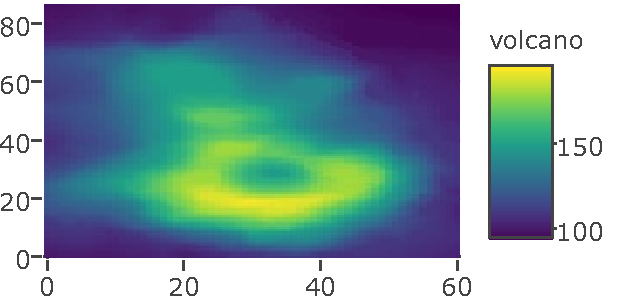
\includegraphics{bookdown_files/figure-latex/unnamed-chunk-5-1.pdf}
\caption{}
\end{figure}

\begin{rmdtip}
\textbf{plotly} uses the \href{http://www.htmlwidgets.org/}{htmlwidget}
framework, which allows plots to work seamlessly and consistently in
various contexts (e.g., R Markdown documents, shiny apps, inside
RStudio, or any other R command prompt) without an internet connection.
IPython/Jupyter notebook users should wrap plots with the
\texttt{embed\_notebook()} function to embed them inline inside a
notebook.
\end{rmdtip}

\section*{plot.ly for collaboration}\label{plot.ly-for-collaboration}
\addcontentsline{toc}{section}{plot.ly for collaboration}

\href{https://plot.ly/}{plot.ly} subscribers can use the
\texttt{plotly\_POST()} function to publish plots from R onto plotly's
web platform. This platform makes it very easy to host/share your
graphs, collaborate with others, and is free to use for public
graphs.\footnote{If you need privacy or customer support,
  \href{https://plot.ly/products/cloud/}{pricing options}} Once a plot
is hosted on your account, others may copy/fork your graph to their
account (with the right permissions) using a friendly user-interface.
Here is a quick demonstration of that workflow from inside RStudio:

\begin{rmdtip}
As long as you can view a plot hosted on \url{http://plot.ly}, you can
bring the data behind with plot into R via the \texttt{get\_figure()}
function. This makes it easy to access and modify plots created with
\emph{any} plotly.js interface (e.g., Python, MATLAB, Julia, Scala, etc)
from your R console.
\end{rmdtip}

Not only is this web-based user-interface to plotly.js useful for
collaborating with others, but it is also useful for completing tasks
that are cumbersome to do at the command-line. For instance, annotations
can be added to any plot via a point-and-click interface:

\chapter{Two approaches, one object}\label{two-approaches-one-object}

There are two main ways to initiate a plotly object in R. The
\texttt{plot\_ly()} function transforms \emph{data} into a plotly
object, while the \texttt{ggplotly()} function transforms a \emph{ggplot
object} into a plotly object \citep{ggplot2}; \citep{plotly}. Regardless
how plotly object is created, printing it results in an interactive
web-based visualization with tooltips, zooming, and panning enabled by
default. It is also possible to enable more advanced interactive
techniques, such as \protect\hyperlink{animation}{animation} and
\protect\hyperlink{linked-highlighting}{linked highlighting}. This
chapter discusses some of the philosophy behind each approach, explores
some of their similarities, and explains why understanding both
approaches is extremely powerful.

The initial inspiration for the \texttt{plot\_ly()} function was to
support \href{https://github.com/plotly/plotly.js}{plotly.js} chart
types that \textbf{ggplot2} doesn't support, such as 3D surface and mesh
plots. Over time, this effort snowballed into an interface to the entire
plotly.js graphing library with additional abstractions inspired by the
grammar of graphics \citep{Wilkinson:2005}. This newer ``non-ggplot2''
interface to plotly.js is currently not, and may never be, as fully
featured as \textbf{ggplot2}. Since we can already translate a fairly
large amount of ggplot objects to plotly objects, I'd rather not
reinvent those same abstractions, and focus providing useful tools for
\href{advanced-interactive-techniques}{advanced interactive graphics}.

The next section uses a case study to introduce some of the similarities
between \texttt{ggplotly()} and \texttt{plot\_ly()}, dives into the
cognitive framework behind \texttt{plot\_ly()}, and also demonstrates
how to \protect\hyperlink{extending-ggplotly}{extend
\texttt{ggplotly()}} with functions that can modify plotly objects.

\section{A case study of housing sales in
Texas}\label{a-case-study-of-housing-sales-in-texas}

The \textbf{plotly} package depends on \textbf{ggplot2} which bundles a
data set on monthly housing sales in Texan cities acquired from the
\href{http://recenter.tamu.edu/}{TAMU real estate center}. After the
loading the package, the data is ``lazily loaded'' into your session, so
you may reference it by name:

\begin{Shaded}
\begin{Highlighting}[]
\KeywordTok{library}\NormalTok{(plotly)}
\NormalTok{txhousing}
\CommentTok{#> # A tibble: 8,602 × 9}
\CommentTok{#>      city  year month sales   volume median listings inventory  date}
\CommentTok{#>     <chr> <int> <int> <dbl>    <dbl>  <dbl>    <dbl>     <dbl> <dbl>}
\CommentTok{#> 1 Abilene  2000     1    72  5380000  71400      701       6.3  2000}
\CommentTok{#> 2 Abilene  2000     2    98  6505000  58700      746       6.6  2000}
\CommentTok{#> 3 Abilene  2000     3   130  9285000  58100      784       6.8  2000}
\CommentTok{#> 4 Abilene  2000     4    98  9730000  68600      785       6.9  2000}
\CommentTok{#> 5 Abilene  2000     5   141 10590000  67300      794       6.8  2000}
\CommentTok{#> 6 Abilene  2000     6   156 13910000  66900      780       6.6  2000}
\CommentTok{#> # ... with 8,596 more rows}
\end{Highlighting}
\end{Shaded}

In attempt to understand house price behavior over time, we could plot
\texttt{date} on x, \texttt{median} on y, and group the lines connecting
these x/y pairs by \texttt{city}. Using \textbf{ggplot2}, we can
\emph{initiate} a ggplot object with the \texttt{ggplot()} function
which accepts a data frame and a mapping from data variables to visual
aesthetics. By just initiating the object, \textbf{ggplot2} won't know
how to geometrically represent the mapping until we add a layer to the
plot via one of \texttt{geom\_*()} (or \texttt{stat\_*()}) functions (in
this case, we want \texttt{geom\_line()}). In this case, it is also a
good idea to specify alpha transparency so that 5 lines plotted on top
of each other appear as solid black, to help avoid overplotting.

\begin{rmdtip}
If you're new to \textbf{ggplot2}, the
\href{https://www.rstudio.com/wp-content/uploads/2015/12/ggplot2-cheatsheet-2.0.pdf}{ggplot2
cheatsheet} provides a nice quick overview. The
\href{http://docs.ggplot2.org/current/}{online docs} or
\href{http://www.cookbook-r.com/Graphs/}{R graphics cookbook} are
helpful for learning by example, and the
\href{https://github.com/hadley/ggplot2-book}{ggplot2 book} provides a
nice overview of the conceptual underpinnings.
\end{rmdtip}

\begin{Shaded}
\begin{Highlighting}[]
\NormalTok{p <-}\StringTok{ }\KeywordTok{ggplot}\NormalTok{(txhousing, }\KeywordTok{aes}\NormalTok{(date, median)) +}
\StringTok{  }\KeywordTok{geom_line}\NormalTok{(}\KeywordTok{aes}\NormalTok{(}\DataTypeTok{group =} \NormalTok{city), }\DataTypeTok{alpha =} \FloatTok{0.2}\NormalTok{)}
\end{Highlighting}
\end{Shaded}

\subsection{\texorpdfstring{The \texttt{ggplotly()}
function}{The ggplotly() function}}\label{ggplotly}

Now that we have a valid \textbf{ggplot2} object, \texttt{p}, the
\textbf{plotly} package provides the \texttt{ggplotly()} function which
converts a ggplot object to a plotly object. By default, it supplies the
entire aesthetic mapping to the tooltip, but the \texttt{tooltip}
argument provides a way to restrict tooltip info to a subset of that
mapping. Furthermore, in cases where the statistic of a layer is
something other than the identity function (e.g., \texttt{geom\_bin2d()}
and \texttt{geom\_hex()}), relevant ``intermediate'' variables generated
in the process are also supplied to the tooltip. This provides a nice
mechanism for decoding visual aesthetics (e.g., color) used to represent
a measure of interest (e.g, count/value). In Figure \ref{fig:ggsubplot},
the \texttt{subplot()} function from the \textbf{plotly} package
(discussed in more detail in \protect\hyperlink{subplot}{subplots}),
which accepts a collection of ggplot and/or plotly objects, helps to
concisely display tooltips for a number of scenarios, and how to
suppress them.

\begin{Shaded}
\begin{Highlighting}[]
\KeywordTok{subplot}\NormalTok{(}
  \NormalTok{p, }\KeywordTok{ggplotly}\NormalTok{(p, }\DataTypeTok{tooltip =} \StringTok{"city"}\NormalTok{), }
  \KeywordTok{ggplot}\NormalTok{(txhousing, }\KeywordTok{aes}\NormalTok{(date, median)) +}\StringTok{ }\KeywordTok{geom_bin2d}\NormalTok{(),}
  \KeywordTok{ggplot}\NormalTok{(txhousing, }\KeywordTok{aes}\NormalTok{(date, median)) +}\StringTok{ }\KeywordTok{geom_hex}\NormalTok{(),}
  \DataTypeTok{nrows =} \DecValTok{2}\NormalTok{, }\DataTypeTok{shareX =} \OtherTok{TRUE}\NormalTok{, }\DataTypeTok{shareY =} \OtherTok{TRUE}\NormalTok{,}
  \DataTypeTok{titleY =} \OtherTok{FALSE}\NormalTok{, }\DataTypeTok{titleX =} \OtherTok{FALSE}
\NormalTok{)}
\end{Highlighting}
\end{Shaded}

\begin{figure}[htbp]
\centering
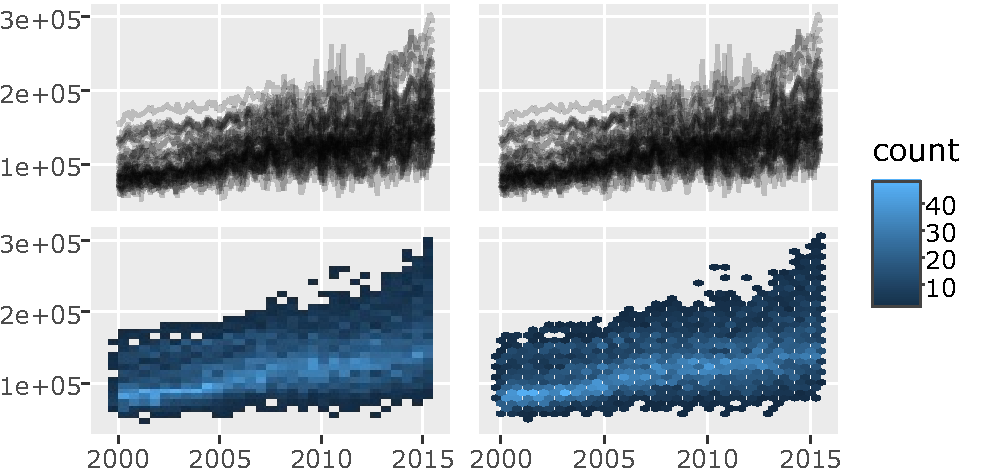
\includegraphics{bookdown_files/figure-latex/ggsubplot-1.pdf}
\caption{\label{fig:ggsubplot}Monthly median house price in the state of
Texas. The top row displays the raw data (by city) and the bottom row
shows 2D binning on the raw data. The binning is helpful for showing the
overall trend, but hovering on the lines in the top row helps reveal
more detailed information about each city.}
\end{figure}

\begin{rmdtip}
Although \textbf{ggplot2} does not have a \texttt{text} aesthetic, the
\texttt{ggplotly()} function recognizes this aesthetic and displays it
in the tooltip by default. In addition to providing a way to supply
``meta'' information, it also provides a way to customize your tooltips
(do this by restricting the tooltip to the text aesthetic --
\texttt{ggplotly(p,\ tooltip\ =\ "text")})
\end{rmdtip}

The \texttt{ggplotly()} function translates most things that you can do
in \textbf{ggplot2}, but not quite everything. To help demonstrate the
coverage, I've built a
\href{http://ropensci.github.io/plotly/ggplot2}{plotly version of the
ggplot2 docs}. This version of the docs displays the \texttt{ggplotly()}
version of each plot in a static form (to reduce page loading time), but
you can click any plot to view its interactive version. The next section
deomnstrates how to create plotly.js visualizations via the R package,
without \textbf{ggplot2}, via \protect\hyperlink{plot_ly}{the
\texttt{plot\_ly()} interface}. We'll then leverage those concepts to
\protect\hyperlink{extend-ggplotly}{extend \texttt{ggplotly()}}.

\hypertarget{plot_ly}{\subsection{\texorpdfstring{The
\texttt{plot\_ly()}
interface}{The plot\_ly() interface}}\label{plot_ly}}

\subsubsection{The Layered Grammar of
Graphics}\label{the-layered-grammar-of-graphics}

The cognitive framework underlying the \texttt{plot\_ly()} interface
draw inspiration from the layered grammar of graphics
\citep{Wickham:2010hya}, but in contrast to \texttt{ggplotly()}, it
provides a more flexible and direct interface to
\href{https://github.com/plotly/plotly.js}{plotly.js}. It is more direct
in the sense that it doesn't call \textbf{ggplot2}'s sometimes expensive
plot building routines, and it is more flexible in the sense that data
frames are not required, which is useful for visualizing matrices, as
shown in \protect\hyperlink{get-started}{Get Started}. Although data
frames are not required, it is recommended to use them whenever
possible, especially when constructing a plot with multiple layers or
groups.

When a data frame is associated with a \textbf{plotly} object, it allows
us to manipulate the data underlying that object in the same way we
would directly manipulate the data. Currently, \texttt{plot\_ly()}
borrows semantics from and provides special plotly methods for generic
functions in the \textbf{dplyr} and \textbf{tidyr} packages
\citep{dplyr}; \citep{tidyr}. Most importantly, \texttt{plot\_ly()}
recognizes and preserves groupings created with \textbf{dplyr}'s
\texttt{group\_by()} function.

\begin{Shaded}
\begin{Highlighting}[]
\KeywordTok{library}\NormalTok{(dplyr)}
\NormalTok{tx <-}\StringTok{ }\KeywordTok{group_by}\NormalTok{(txhousing, city)}
\CommentTok{# initiate a plotly object with date on x and median on y}
\NormalTok{p <-}\StringTok{ }\KeywordTok{plot_ly}\NormalTok{(tx, }\DataTypeTok{x =} \NormalTok{~date, }\DataTypeTok{y =} \NormalTok{~median)}
\CommentTok{# plotly_data() returns data associated with a plotly object, note the group attribute!}
\KeywordTok{plotly_data}\NormalTok{(p)}
\CommentTok{#> Source: local data frame [8,602 x 9]}
\CommentTok{#> Groups: city [46]}
\CommentTok{#> }
\CommentTok{#>      city  year month sales   volume median listings inventory  date}
\CommentTok{#>     <chr> <int> <int> <dbl>    <dbl>  <dbl>    <dbl>     <dbl> <dbl>}
\CommentTok{#> 1 Abilene  2000     1    72  5380000  71400      701       6.3  2000}
\CommentTok{#> 2 Abilene  2000     2    98  6505000  58700      746       6.6  2000}
\CommentTok{#> 3 Abilene  2000     3   130  9285000  58100      784       6.8  2000}
\CommentTok{#> 4 Abilene  2000     4    98  9730000  68600      785       6.9  2000}
\CommentTok{#> 5 Abilene  2000     5   141 10590000  67300      794       6.8  2000}
\CommentTok{#> 6 Abilene  2000     6   156 13910000  66900      780       6.6  2000}
\CommentTok{#> # ... with 8,596 more rows}
\end{Highlighting}
\end{Shaded}

Defining groups in this fashion ensures \texttt{plot\_ly()} will produce
at least one graphical mark per group.\footnote{In practice, it's easy
  to forget about ``lingering'' groups (e.g.,
  \texttt{mtcars\ \%\textgreater{}\%\ group\_by(vs,\ am)\ \%\textgreater{}\%\ summarise(s\ =\ sum(mpg))}),
  so in some cases, you may need to \texttt{ungroup()} your data before
  plotting it.} So far we've specified \texttt{x}/\texttt{y} attributes
in the plotly object \texttt{p}, but we have not yet specified the
geometric relation between these x/y pairs. Similar to
\texttt{geom\_line()} in \textbf{ggplot2}, the \texttt{add\_lines()}
function connects (a group of) x/y pairs with lines in the order of
their \texttt{x} values, which is useful when plotting time series as
shown in Figure \ref{fig:houston}.

\begin{Shaded}
\begin{Highlighting}[]
\CommentTok{# add a line highlighting houston}
\KeywordTok{add_lines}\NormalTok{(}
  \CommentTok{# plots one line per city since p knows city is a grouping variable}
  \KeywordTok{add_lines}\NormalTok{(p, }\DataTypeTok{alpha =} \FloatTok{0.2}\NormalTok{, }\DataTypeTok{name =} \StringTok{"Texan Cities"}\NormalTok{, }\DataTypeTok{hoverinfo =} \StringTok{"none"}\NormalTok{),}
  \DataTypeTok{name =} \StringTok{"Houston"}\NormalTok{, }\DataTypeTok{data =} \KeywordTok{filter}\NormalTok{(txhousing, city ==}\StringTok{ "Houston"}\NormalTok{)}
\NormalTok{)}
\end{Highlighting}
\end{Shaded}

\begin{figure}[htbp]
\centering
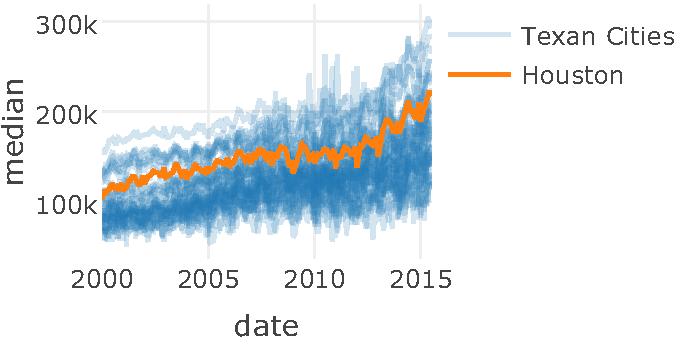
\includegraphics{bookdown_files/figure-latex/houston-1.pdf}
\caption{\label{fig:houston}Monthly median house price in Houston in
comparison to other Texan cities.}
\end{figure}

The \textbf{plotly} package has a collection of \texttt{add\_*()}
functions, all of which inherit attributes defined in
\texttt{plot\_ly()}. These functions also inherit the data associated
with the plotly object provided as input, unless otherwise specified
with the \texttt{data} argument. I prefer to think about
\texttt{add\_*()} functions like a layer in \textbf{ggplot2}, which is
slightly different, but related to a plotly.js trace. In Figure
\ref{fig:houston}, there is a 1-to-1 correspondence between layers and
traces, but \texttt{add\_*()} functions do generate numerous traces
whenever mapping a discrete variable to a visual aesthetic (e.g.,
\href{scatterplots-discrete-color}{color}). In this case, since each
call to \texttt{add\_lines()} generates a single trace, it makes sense
to \texttt{name} the trace, so a sensible legend entry is created.

In the first layer of Figure \ref{fig:houston}, there is one line per
city, but all these lines belong a single trace. We \emph{could have}
produced one trace for each line, but this is way more computationally
expensive because, among other things, each trace produces a legend
entry and tries to display meaningful hover information. It is much more
efficient to render this layer as a single trace with missing values to
differentiate groups. In fact, this is exactly how the group aesthetic
is translated in \texttt{ggplotly()}; otherwise, layers with many groups
(e.g., \texttt{geom\_map()}) would be slow to render.

\subsubsection{The data-plot-pipeline}\label{the-data-plot-pipeline}

Since every \textbf{plotly} function modifies a plotly object (or the
data underlying that object), we can express complex multi-layer plots
as a sequence (or, more specifically, a directed acyclic graph) of data
manipulations and mappings to the visual space. Moreover,
\textbf{plotly} functions are designed to take a plotly object as input,
and return a modified plotly object, making it easy to chain together
operations via the pipe operator (\texttt{\%\textgreater{}\%}) from the
\textbf{magrittr} package \citep{magrittr}. Consequently, we can
re-express Figure \ref{fig:houston} in a much more readable and
understandable fashion.

\begin{Shaded}
\begin{Highlighting}[]
\NormalTok{allCities <-}\StringTok{ }\NormalTok{txhousing %>%}
\StringTok{  }\KeywordTok{group_by}\NormalTok{(city) %>%}
\StringTok{  }\KeywordTok{plot_ly}\NormalTok{(}\DataTypeTok{x =} \NormalTok{~date, }\DataTypeTok{y =} \NormalTok{~median) %>%}
\StringTok{  }\KeywordTok{add_lines}\NormalTok{(}\DataTypeTok{alpha =} \FloatTok{0.2}\NormalTok{, }\DataTypeTok{name =} \StringTok{"Texan Cities"}\NormalTok{, }\DataTypeTok{hoverinfo =} \StringTok{"none"}\NormalTok{)}

\NormalTok{allCities %>%}
\StringTok{  }\KeywordTok{filter}\NormalTok{(city ==}\StringTok{ "Houston"}\NormalTok{) %>%}
\StringTok{  }\KeywordTok{add_lines}\NormalTok{(}\DataTypeTok{name =} \StringTok{"Houston"}\NormalTok{)}
\end{Highlighting}
\end{Shaded}

\begin{figure}[htbp]
\centering
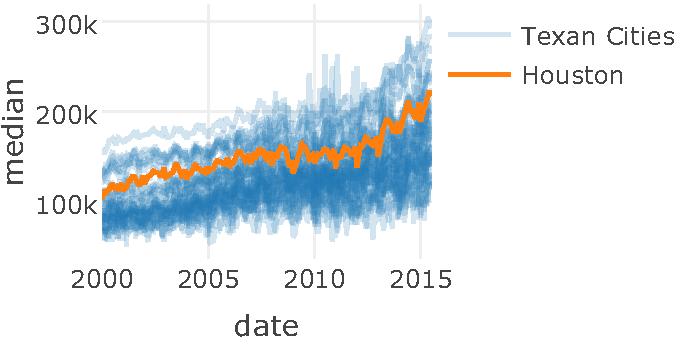
\includegraphics{bookdown_files/figure-latex/unnamed-chunk-15-1.pdf}
\caption{}
\end{figure}

Sometimes the directed acyclic graph property of a pipeline can be too
restrictive for certain types of plots. In this example, after filtering
the data down to Houston, there is no way to recover the original data
inside the pipeline. The \texttt{add\_fun()} function helps to
work-around this restriction\footnote{Credit to Winston Chang and Hadley
  Wickham for this idea. The \texttt{add\_fun()} is very much like
  \texttt{layer\_f()} function in \textbf{ggvis}.} -- it works by
applying a function to the plotly object, but does not affect the data
associated with the plotly object. This effectively provides a way to
isolate data transformations within the pipeline\footnote{Also,
  effectively putting a
  \href{http://www.memecreator.org/meme/yo-dawg-i-heard-u-like-pipelines-so-we-put-a-pipeline-in-your-pipeline}{pipeline
  inside a pipeline}}. Figure \ref{fig:houston-vs-sa} uses this idea to
highlight both Houston and San Antonio.

\begin{Shaded}
\begin{Highlighting}[]
\NormalTok{allCities %>%}
\StringTok{  }\KeywordTok{add_fun}\NormalTok{(function(plot) \{}
    \NormalTok{plot %>%}\StringTok{ }\KeywordTok{filter}\NormalTok{(city ==}\StringTok{ "Houston"}\NormalTok{) %>%}\StringTok{ }\KeywordTok{add_lines}\NormalTok{(}\DataTypeTok{name =} \StringTok{"Houston"}\NormalTok{)}
  \NormalTok{\}) %>%}
\StringTok{  }\KeywordTok{add_fun}\NormalTok{(function(plot) \{}
    \NormalTok{plot %>%}\StringTok{ }\KeywordTok{filter}\NormalTok{(city ==}\StringTok{ "San Antonio"}\NormalTok{) %>%}\StringTok{ }\KeywordTok{add_lines}\NormalTok{(}\DataTypeTok{name =} \StringTok{"San Antonio"}\NormalTok{)}
  \NormalTok{\})}
\end{Highlighting}
\end{Shaded}

\begin{figure}[htbp]
\centering
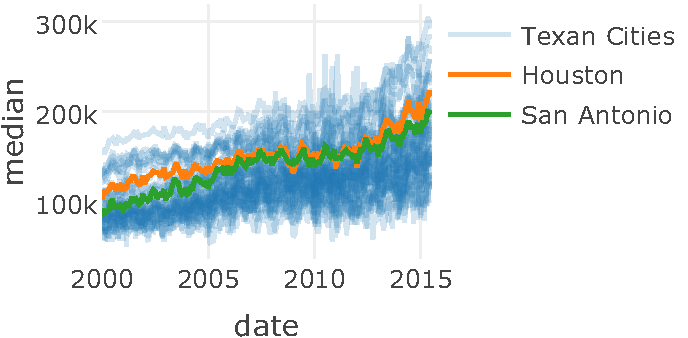
\includegraphics{bookdown_files/figure-latex/houston-vs-sa-1.pdf}
\caption{\label{fig:houston-vs-sa}Monthly median house price in Houston and
San Antonio in comparison to other Texan cities.}
\end{figure}

It is useful to think of the function supplied to \texttt{add\_fun()} as
a ``layer'' function -- a function that accepts a plot object as input,
possibly applies a transformation to the data, and maps that data to
visual objects. To make layering functions more modular, flexible, and
expressive, the \texttt{add\_fun()} allows you to pass additional
arguments to a layer function. Figure \ref{fig:summary} makes use of
this pattern, by creating a reusable function for layering both a
particular city as well as the first, second, and third quartile of
median monthly house sales (by city).

\begin{Shaded}
\begin{Highlighting}[]
\CommentTok{# reusable function for highlighting a particular city}
\NormalTok{layer_city <-}\StringTok{ }\NormalTok{function(plot, name) \{}
  \NormalTok{plot %>%}\StringTok{ }\KeywordTok{filter}\NormalTok{(city ==}\StringTok{ }\NormalTok{name) %>%}\StringTok{ }\KeywordTok{add_lines}\NormalTok{(}\DataTypeTok{name =} \NormalTok{name)}
\NormalTok{\}}

\CommentTok{# reusable function for plotting overall median & IQR}
\NormalTok{layer_iqr <-}\StringTok{ }\NormalTok{function(plot) \{}
  \NormalTok{plot %>%}
\StringTok{    }\KeywordTok{group_by}\NormalTok{(date) %>%}\StringTok{ }
\StringTok{    }\KeywordTok{summarise}\NormalTok{(}
      \DataTypeTok{q1 =} \KeywordTok{quantile}\NormalTok{(median, }\FloatTok{0.25}\NormalTok{, }\DataTypeTok{na.rm =} \OtherTok{TRUE}\NormalTok{),}
      \DataTypeTok{m =} \KeywordTok{median}\NormalTok{(median, }\DataTypeTok{na.rm =} \OtherTok{TRUE}\NormalTok{),}
      \DataTypeTok{q3 =} \KeywordTok{quantile}\NormalTok{(median, }\FloatTok{0.75}\NormalTok{, }\DataTypeTok{na.rm =} \OtherTok{TRUE}\NormalTok{)}
    \NormalTok{) %>%}
\StringTok{    }\KeywordTok{add_lines}\NormalTok{(}\DataTypeTok{y =} \NormalTok{~m, }\DataTypeTok{name =} \StringTok{"median"}\NormalTok{, }\DataTypeTok{color =} \KeywordTok{I}\NormalTok{(}\StringTok{"black"}\NormalTok{)) %>%}
\StringTok{    }\KeywordTok{add_ribbons}\NormalTok{(}\DataTypeTok{ymin =} \NormalTok{~q1, }\DataTypeTok{ymax =} \NormalTok{~q3, }\DataTypeTok{name =} \StringTok{"IQR"}\NormalTok{, }\DataTypeTok{color =} \KeywordTok{I}\NormalTok{(}\StringTok{"black"}\NormalTok{))}
\NormalTok{\}}

\NormalTok{allCities %>%}
\StringTok{  }\KeywordTok{add_fun}\NormalTok{(layer_iqr) %>%}
\StringTok{  }\KeywordTok{add_fun}\NormalTok{(layer_city, }\StringTok{"Houston"}\NormalTok{) %>%}
\StringTok{  }\KeywordTok{add_fun}\NormalTok{(layer_city, }\StringTok{"San Antonio"}\NormalTok{)}
\end{Highlighting}
\end{Shaded}

\begin{figure}[htbp]
\centering
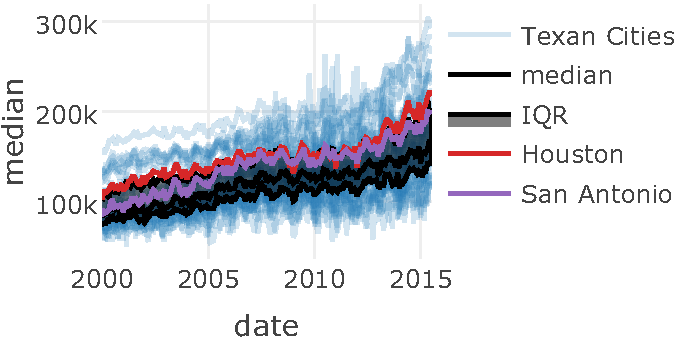
\includegraphics{bookdown_files/figure-latex/summary-1.pdf}
\caption{\label{fig:summary}First, second, and third quartile of median
monthly house pirce in Texas.}
\end{figure}

A layering function does not have to be a data-plot-pipeline itself. Its
only requirement on a layering function is that the first argument is a
plot object and it returns a plot object. This provides an opportunity
to say, fit a model to the plot data, extract the model components you
desire, and map those components to visuals. Furthermore, since
\textbf{plotly}'s \texttt{add\_*()} functions don't require a
data.frame, you can supply those components directly to attributes (as
long as they are well-defined), as done in Figure \ref{fig:forecast} via
the \textbf{forecast} package \citep{forecast}.

\begin{Shaded}
\begin{Highlighting}[]
\KeywordTok{library}\NormalTok{(forecast)}
\NormalTok{layer_forecast <-}\StringTok{ }\NormalTok{function(plot) \{}
  \NormalTok{d <-}\StringTok{ }\KeywordTok{plotly_data}\NormalTok{(plot)}
  \NormalTok{series <-}\StringTok{ }\KeywordTok{with}\NormalTok{(d, }
    \KeywordTok{ts}\NormalTok{(median, }\DataTypeTok{frequency =} \DecValTok{12}\NormalTok{, }\DataTypeTok{start =} \KeywordTok{c}\NormalTok{(}\DecValTok{2000}\NormalTok{, }\DecValTok{1}\NormalTok{), }\DataTypeTok{end =} \KeywordTok{c}\NormalTok{(}\DecValTok{2015}\NormalTok{, }\DecValTok{7}\NormalTok{))}
  \NormalTok{)}
  \NormalTok{fore <-}\StringTok{ }\KeywordTok{forecast}\NormalTok{(}\KeywordTok{ets}\NormalTok{(series), }\DataTypeTok{h =} \DecValTok{48}\NormalTok{, }\DataTypeTok{level =} \KeywordTok{c}\NormalTok{(}\DecValTok{80}\NormalTok{, }\DecValTok{95}\NormalTok{))}
  \NormalTok{plot %>%}
\StringTok{    }\KeywordTok{add_ribbons}\NormalTok{(}\DataTypeTok{x =} \KeywordTok{time}\NormalTok{(fore$mean), }\DataTypeTok{ymin =} \NormalTok{fore$lower[, }\DecValTok{2}\NormalTok{],}
                \DataTypeTok{ymax =} \NormalTok{fore$upper[, }\DecValTok{2}\NormalTok{], }\DataTypeTok{color =} \KeywordTok{I}\NormalTok{(}\StringTok{"gray95"}\NormalTok{), }
                \DataTypeTok{name =} \StringTok{"95% confidence"}\NormalTok{, }\DataTypeTok{inherit =} \OtherTok{FALSE}\NormalTok{) %>%}
\StringTok{    }\KeywordTok{add_ribbons}\NormalTok{(}\DataTypeTok{x =} \KeywordTok{time}\NormalTok{(fore$mean), }\DataTypeTok{ymin =} \NormalTok{fore$lower[, }\DecValTok{1}\NormalTok{],}
                \DataTypeTok{ymax =} \NormalTok{fore$upper[, }\DecValTok{1}\NormalTok{], }\DataTypeTok{color =} \KeywordTok{I}\NormalTok{(}\StringTok{"gray80"}\NormalTok{), }
                \DataTypeTok{name =} \StringTok{"80% confidence"}\NormalTok{, }\DataTypeTok{inherit =} \OtherTok{FALSE}\NormalTok{) %>%}
\StringTok{    }\KeywordTok{add_lines}\NormalTok{(}\DataTypeTok{x =} \KeywordTok{time}\NormalTok{(fore$mean), }\DataTypeTok{y =} \NormalTok{fore$mean, }\DataTypeTok{color =} \KeywordTok{I}\NormalTok{(}\StringTok{"blue"}\NormalTok{), }
              \DataTypeTok{name =} \StringTok{"prediction"}\NormalTok{)}
\NormalTok{\}}

\NormalTok{txhousing %>%}
\StringTok{  }\KeywordTok{group_by}\NormalTok{(city) %>%}
\StringTok{  }\KeywordTok{plot_ly}\NormalTok{(}\DataTypeTok{x =} \NormalTok{~date, }\DataTypeTok{y =} \NormalTok{~median) %>%}
\StringTok{  }\KeywordTok{add_lines}\NormalTok{(}\DataTypeTok{alpha =} \FloatTok{0.2}\NormalTok{, }\DataTypeTok{name =} \StringTok{"Texan Cities"}\NormalTok{, }\DataTypeTok{hoverinfo =} \StringTok{"none"}\NormalTok{) %>%}
\StringTok{  }\KeywordTok{add_fun}\NormalTok{(layer_iqr) %>%}
\StringTok{  }\KeywordTok{add_fun}\NormalTok{(layer_forecast)}
\end{Highlighting}
\end{Shaded}

\begin{figure}[htbp]
\centering
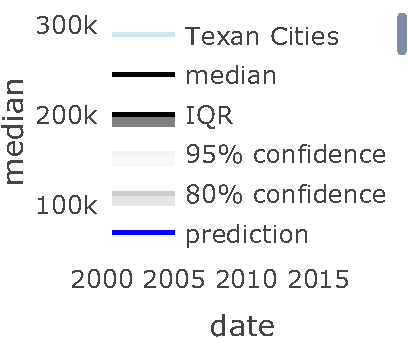
\includegraphics{bookdown_files/figure-latex/forecast-1.pdf}
\caption{\label{fig:forecast}Layering on a 4-year forecast from a
exponential smoothing state space model.}
\end{figure}

In summary, the ``data-plot-pipeline'' is desirable for a number of
reasons: (1) makes your code easier to read and understand, (2)
encourages you to think of both your data and plots using a single,
uniform data structure, which (3) makes it easy to combine and reuse
different pipelines, and (4) provides a natural mechanism for
implementing the pipeline(s) necessary in interactive graphics system
with support for \protect\hyperlink{linked-highlighting}{Linked
Highlighting} \citep{plumbing}. As it turns out, we can even use these
ideas when creating a plotly object via \texttt{ggplotly()}, as discused
in the next section \href{extending-ggplotly()}{Extending
\texttt{ggplotly()}}.

\hypertarget{extending-ggplotly}{\section{\texorpdfstring{Extending
\texttt{ggplotly()}}{Extending ggplotly()}}\label{extending-ggplotly}}

\subsection{Customizing the layout}\label{customizing-the-layout}

Since the \texttt{ggplotly()} function returns a plotly object, we can
manipulate that object in the same way that we would manipulate an
object created with \texttt{plot\_ly()}. A simple and obviously useful
application of this is to specify interaction modes, like plotly.js'
\href{https://plot.ly/r/reference/\#layout-hovermode}{layout.hovermode}.

\begin{Shaded}
\begin{Highlighting}[]
\NormalTok{p <-}\StringTok{ }\KeywordTok{ggplot}\NormalTok{(}\KeywordTok{fortify}\NormalTok{(gold), }\KeywordTok{aes}\NormalTok{(x, y)) +}\StringTok{ }\KeywordTok{geom_line}\NormalTok{()}
\NormalTok{gg <-}\StringTok{ }\KeywordTok{ggplotly}\NormalTok{(p)}
\KeywordTok{layout}\NormalTok{(gg, }\DataTypeTok{hovermode =} \StringTok{"x"}\NormalTok{)}
\end{Highlighting}
\end{Shaded}

\begin{figure}[htbp]
\centering
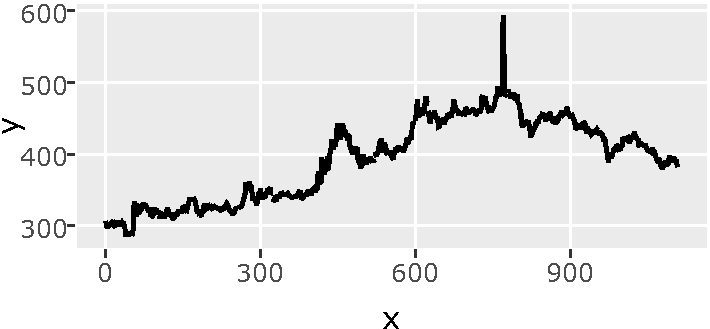
\includegraphics{bookdown_files/figure-latex/unnamed-chunk-16-1.pdf}
\caption{}
\end{figure}

We can also easily add a range slider to the x-axis, which allows you to
zoom on the x-axis, without losing the global context. This is quite
useful for quickly altering the limits of your plot to achieve an
optimal aspect ratio for your data \citep{banking}, without losing the
global perspective.

\begin{Shaded}
\begin{Highlighting}[]
\KeywordTok{rangeslider}\NormalTok{(gg)}
\end{Highlighting}
\end{Shaded}

\begin{figure}[htbp]
\centering
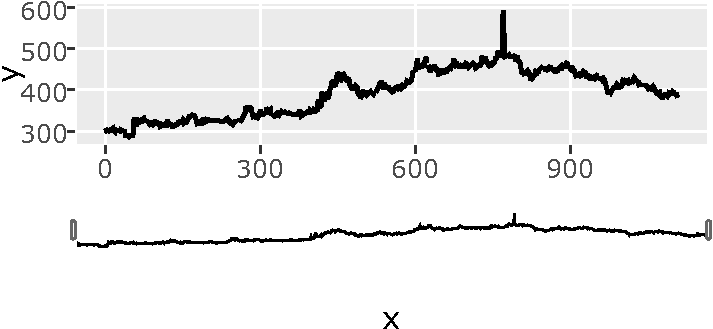
\includegraphics{bookdown_files/figure-latex/unnamed-chunk-17-1.pdf}
\caption{}
\end{figure}

Since a single plotly object can only have one layout, modifying the
layout of \texttt{ggplotly()} is fairly easy, but it's trickier to
\protect\hyperlink{adding-layers}{add} and
\protect\hyperlink{modifying-layers}{modify} layers.

\hypertarget{adding-layers}{\subsection{Adding
layers}\label{adding-layers}}

Since \texttt{ggplotly()} returns a plotly object, and plotly objects
have data associated with them, we can effectively associate data from a
ggplot object with a plotly object, before or after summary statistics
have been applied. Since each ggplot layer owns a data frame, it is
useful to have some way to specify the particular layer of data of
interest, which is the point of the \texttt{layerData} argument in
\texttt{ggplotly()}. Also, when a particular layer applies a summary
statistic (e.g., \texttt{geom\_bin()}), or applies a model (e.g.,
\texttt{geom\_smooth()}) to the data, it might be useful to access the
output of that transformation, which is the point of the
\texttt{originalData} argument in \texttt{ggplotly()}.

\begin{Shaded}
\begin{Highlighting}[]
\NormalTok{p <-}\StringTok{ }\KeywordTok{ggplot}\NormalTok{(mtcars, }\KeywordTok{aes}\NormalTok{(}\DataTypeTok{x =} \NormalTok{wt, }\DataTypeTok{y =} \NormalTok{mpg)) +}
\StringTok{   }\KeywordTok{geom_point}\NormalTok{() +}\StringTok{ }\KeywordTok{geom_smooth}\NormalTok{()}
\NormalTok{p %>%}
\StringTok{  }\KeywordTok{ggplotly}\NormalTok{(}\DataTypeTok{layerData =} \DecValTok{2}\NormalTok{, }\DataTypeTok{originalData =} \OtherTok{FALSE}\NormalTok{) %>%}
\StringTok{  }\KeywordTok{plotly_data}\NormalTok{()}
\CommentTok{#> # A tibble: 80 × 13}
\CommentTok{#>       x     y  ymin  ymax    se PANEL group  colour   fill  size linetype}
\CommentTok{#> * <dbl> <dbl> <dbl> <dbl> <dbl> <int> <int>   <chr>  <chr> <dbl>    <dbl>}
\CommentTok{#> 1  1.51  32.1  28.1  36.0  1.92     1    -1 #3366FF grey60     1        1}
\CommentTok{#> 2  1.56  31.7  28.2  35.2  1.72     1    -1 #3366FF grey60     1        1}
\CommentTok{#> 3  1.61  31.3  28.1  34.5  1.54     1    -1 #3366FF grey60     1        1}
\CommentTok{#> 4  1.66  30.9  28.0  33.7  1.39     1    -1 #3366FF grey60     1        1}
\CommentTok{#> 5  1.71  30.5  27.9  33.0  1.26     1    -1 #3366FF grey60     1        1}
\CommentTok{#> 6  1.76  30.0  27.7  32.4  1.16     1    -1 #3366FF grey60     1        1}
\CommentTok{#> # ... with 74 more rows, and 2 more variables: weight <dbl>, alpha <dbl>}
\end{Highlighting}
\end{Shaded}

This is the dataset ggplot2 uses to actually draw the fitted values (as
a line) and standard error bounds (as a ribbon). Figure
\ref{fig:se-annotations} uses this data to add additional information
about the model fit; in particular, it adds a vertical lines and
annotations at the x-values that are associated with the highest and
lowest amount uncertainty in y.

\begin{Shaded}
\begin{Highlighting}[]
\NormalTok{p %>%}
\StringTok{  }\KeywordTok{ggplotly}\NormalTok{(}\DataTypeTok{layerData =} \DecValTok{2}\NormalTok{, }\DataTypeTok{originalData =} \NormalTok{F) %>%}
\StringTok{  }\KeywordTok{add_fun}\NormalTok{(function(p) \{}
    \NormalTok{p %>%}\StringTok{ }\KeywordTok{slice}\NormalTok{(}\KeywordTok{which.max}\NormalTok{(se)) %>%}
\StringTok{      }\KeywordTok{add_segments}\NormalTok{(}\DataTypeTok{x =} \NormalTok{~x, }\DataTypeTok{xend =} \NormalTok{~x, }\DataTypeTok{y =} \NormalTok{~ymin, }\DataTypeTok{yend =} \NormalTok{~ymax) %>%}
\StringTok{      }\KeywordTok{add_annotations}\NormalTok{(}\StringTok{"Maximum uncertainty"}\NormalTok{, }\DataTypeTok{ax =} \DecValTok{60}\NormalTok{)}
  \NormalTok{\}) %>%}
\StringTok{  }\KeywordTok{add_fun}\NormalTok{(function(p) \{}
    \NormalTok{p %>%}\StringTok{ }\KeywordTok{slice}\NormalTok{(}\KeywordTok{which.min}\NormalTok{(se)) %>%}
\StringTok{      }\KeywordTok{add_segments}\NormalTok{(}\DataTypeTok{x =} \NormalTok{~x, }\DataTypeTok{xend =} \NormalTok{~x, }\DataTypeTok{y =} \NormalTok{~ymin, }\DataTypeTok{yend =} \NormalTok{~ymax) %>%}
\StringTok{      }\KeywordTok{add_annotations}\NormalTok{(}\StringTok{"Minimum uncertainty"}\NormalTok{)}
  \NormalTok{\})}
\end{Highlighting}
\end{Shaded}

\begin{figure}[htbp]
\centering
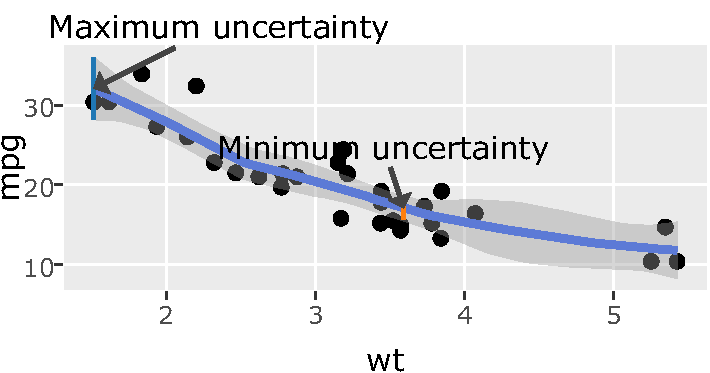
\includegraphics{bookdown_files/figure-latex/se-annotations-1.pdf}
\caption{\label{fig:se-annotations}Leveraging data associated with a
\texttt{geom\_smooth()} layer to display additional information about
the model fit.}
\end{figure}

Although it is not used in this example, it worth noting that when
adding plotly layers to the output of \texttt{ggplotly()}, it will
inherit the global mapping by default, which may or may not be desired,
but the \texttt{inherit} argument in any of the \texttt{add\_*()}
functions may be set to \texttt{FALSE} to avoid this behavoir.

\hypertarget{modifying-layers}{\subsection{Modifying
layers}\label{modifying-layers}}

As mentioned previously, \texttt{ggplotly()} translates each ggplot2
layer into one or more plotly.js traces. In this translation, it is
forced to make a number of assumptions about trace attribute values that
may or may not be appropriate for the use case. The \texttt{style()}
function is useful in this scenario, as it provides a way to modify
trace attribute values in a plotly object. Before using it, you may want
to inspect the actual traces in a given plotly object using the
\texttt{plotly\_json()} function. This function uses the
\textbf{listviewer} package to display a convenient interactive view of
the JSON object sent to plotly.js \citep{listviewer}. By clicking on the
arrow next to the data element, you can see the traces (data) behind the
plot. In this case, we have three traces: one for the
\texttt{geom\_point()} layer and two for the \texttt{geom\_smooth()}
layer.

\begin{Shaded}
\begin{Highlighting}[]
\KeywordTok{plotly_json}\NormalTok{(p)}
\end{Highlighting}
\end{Shaded}

\begin{figure}[htbp]
\centering
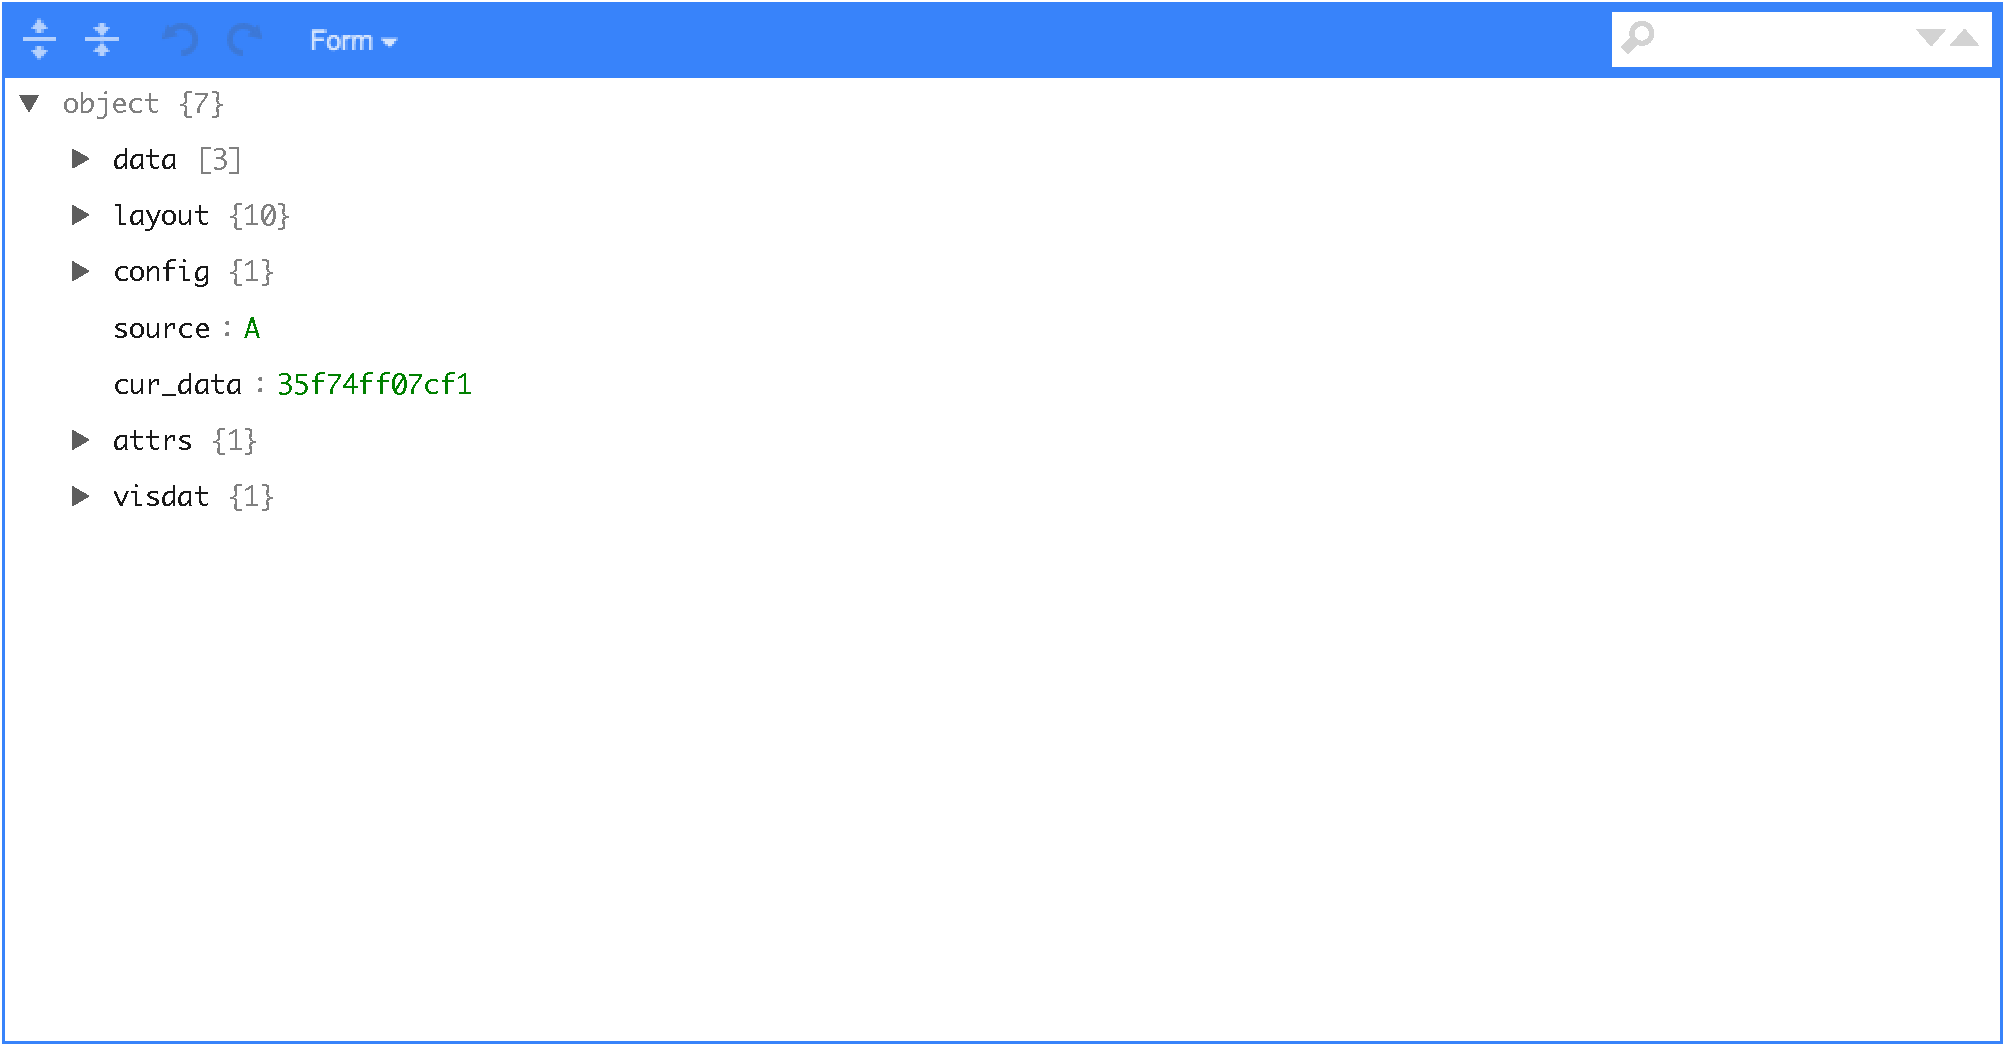
\includegraphics{bookdown_files/figure-latex/listviewer-1.pdf}
\caption{\label{fig:listviewer}Using listviewer to inspect a plotly object.}
\end{figure}

Say, for example, we'd like to display information when hovering over
points, but not when hovering over the fitted values or error bounds.
The ggplot2 API has no semantics for making this distinction, but this
is easily done in plotly.js by setting the
\href{https://plot.ly/r/reference/\#scatter-hoverinfo}{hoverinfo}
attribute to \texttt{"none"}. Since the fitted values or error bounds
are contained in the second and third traces, we can hide the
information on just these traces using the \texttt{traces} attribute in
the \texttt{style()} function:

\begin{Shaded}
\begin{Highlighting}[]
\KeywordTok{style}\NormalTok{(p, }\DataTypeTok{hoverinfo =} \StringTok{"none"}\NormalTok{, }\DataTypeTok{traces =} \DecValTok{2}\NormalTok{:}\DecValTok{3}\NormalTok{)}
\end{Highlighting}
\end{Shaded}

\begin{figure}[htbp]
\centering
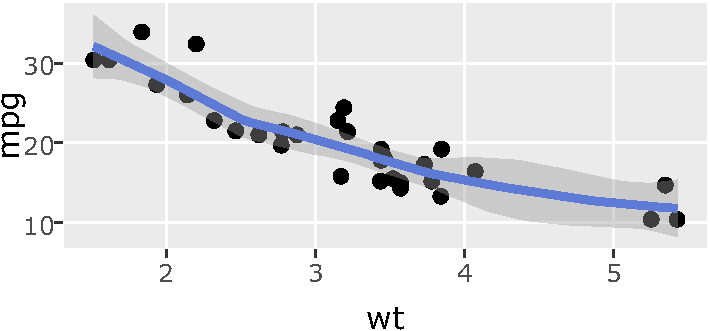
\includegraphics{bookdown_files/figure-latex/unnamed-chunk-20-1.pdf}
\caption{}
\end{figure}

\section{Choosing an interface}\label{choosing-an-interface}

\begin{enumerate}
\def\labelenumi{\arabic{enumi}.}
\tightlist
\item
  ggplot2 requires data frame(s) and can be inefficient (especially for
  time series).
\item
  ggplot2 does not have a functional interface (making it awkward to
  combine with modern functional interfaces such as dplyr), and does not
  satisfy
  \href{https://en.wikipedia.org/wiki/Referential_transparency}{referential
  transparency} (making it easier to program with -- for more details,
  see )
\item
  \texttt{ggplotly()} tries to replicate \emph{exactly} what you see in
  the corresponding static ggplot2 graph. To do so, it sends axis tick
  information to plotly as
  \href{https://plot.ly/r/reference/\#layout-xaxis-tickvals}{tickvals}/\href{https://plot.ly/r/reference/\#layout-xaxis-ticktext}{ticktext}
  properties, and consequently, axis ticks do not update on zoom events.
\item
  ggplot2's interface wasn't designed for interactive graphics. Directly
  extending the grammar to support more advanced types of interaction
  (e.g., linked brushing) is a risky endeavor.
\end{enumerate}

\chapter{The plotly cookbook}\label{the-plotly-cookbook}

This chapter demonstrates the capabilities of \texttt{plot\_ly()}
through a series of examples. The \texttt{plot\_ly()} function does
provide a direct interface to plotly.js, so anything in
\href{https://plot.ly/r/reference/}{the figure reference} can be
specified via \texttt{plot\_ly()}, but this chapter will focus more on
the semantics unique to the R package that can't be found on the figure
reference. Along the way, we will touch on some best practices in
visualization.

\hypertarget{scatter-traces}{\section{Scatter
traces}\label{scatter-traces}}

A plotly visualization is composed of one (or more) trace(s), and every
trace has a \texttt{type}. The default trace type, ``scatter'', can be
used to draw a large amount of geometries, and actually powers many of
the \texttt{add\_*()} functions such as \texttt{add\_markers()},
\texttt{add\_lines()}, \texttt{add\_paths()}, \texttt{add\_segments()},
\texttt{add\_ribbons()}, and \texttt{add\_polygons()}. Among other
things, these functions make assumptions about the
\href{https://plot.ly/r/reference/\#scatter-mode}{mode} of the scatter
trace, but any valid attribute(s) listed under the
\href{https://plot.ly/r/reference/\#scatter}{scatter section of the
figure reference} may be used to override defaults.

You may notice some arguments are related to items in the in the figure
reference, but are not listed (e.g., \texttt{color}/\texttt{colors},
\texttt{symbol}/\texttt{symbols}, \texttt{linetype}/\texttt{linetypes},
\texttt{size}/\texttt{sizes}). These arguments (documented on the help
page \texttt{help(plot\_ly)}) are unique to the R package and make it
easier to scale data values to visual aesthetics. Generally speaking,
the singular form of the argument defines the domain of the scale (data)
and the plural form defines the range of the scale (visuals). To make it
easier to alter default visual aesthetics (e.g., change all points from
blue to black), interprets ``AsIs'' values (values wrapped with the
\texttt{I()} function) as values that already live in visual space, and
thus do not need to be scaled. The next section on scatterplots explores
detailed use of the \texttt{color}/\texttt{colors},
\texttt{symbol}/\texttt{symbols}, \& \texttt{size}/\texttt{sizes}
arguments. The section on \protect\hyperlink{line-plots}{lineplots}
explores detailed use of the \texttt{linetype}/\texttt{linetypes}.

\hypertarget{scatterplots}{\subsection{Scatterplots}\label{scatterplots}}

The scatterplot is useful for visualizing the correlation between two
quantitative variables. If you supply a numeric vector for x and y in
\texttt{plot\_ly()}, it defaults to a scatterplot, but you can also be
explicit about adding a layer of markers/points via the
\texttt{add\_markers()} function. A common problem with scatterplots is
overplotting, meaning that there are multiple observations occupying the
same (or similar) x/y locations. There are a few ways to combat
overplotting including: alpha transparency, hollow symbols, and
\protect\hyperlink{rectangular-binning-in-R}{2D density estimation}.
Figure \ref{fig:scatterplots} shows how alpha transparency and hollow
symbols can provide an improvment over the default.

\begin{Shaded}
\begin{Highlighting}[]
\KeywordTok{subplot}\NormalTok{(}
  \KeywordTok{plot_ly}\NormalTok{(mpg, }\DataTypeTok{x =} \NormalTok{~cty, }\DataTypeTok{y =} \NormalTok{~hwy, }\DataTypeTok{name =} \StringTok{"default"}\NormalTok{),}
  \KeywordTok{plot_ly}\NormalTok{(mpg, }\DataTypeTok{x =} \NormalTok{~cty, }\DataTypeTok{y =} \NormalTok{~hwy) %>%}\StringTok{ }\KeywordTok{add_markers}\NormalTok{(}\DataTypeTok{alpha =} \FloatTok{0.2}\NormalTok{, }\DataTypeTok{name =} \StringTok{"alpha"}\NormalTok{),}
  \KeywordTok{plot_ly}\NormalTok{(mpg, }\DataTypeTok{x =} \NormalTok{~cty, }\DataTypeTok{y =} \NormalTok{~hwy) %>%}\StringTok{ }\KeywordTok{add_markers}\NormalTok{(}\DataTypeTok{symbol =} \KeywordTok{I}\NormalTok{(}\DecValTok{1}\NormalTok{), }\DataTypeTok{name =} \StringTok{"hollow"}\NormalTok{)}
\NormalTok{)}
\end{Highlighting}
\end{Shaded}

\begin{figure}[htbp]
\centering
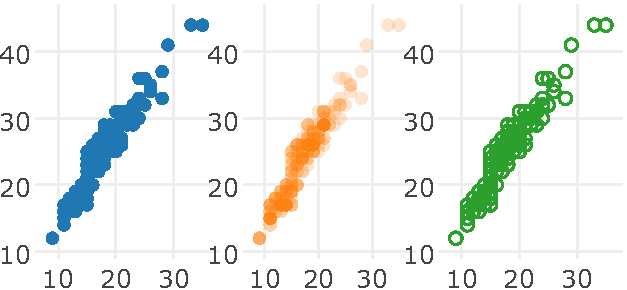
\includegraphics{bookdown_files/figure-latex/scatterplots-1.pdf}
\caption{\label{fig:scatterplots}Three versions of a basic scatterplot}
\end{figure}

In Figure \ref{fig:scatterplots}, hollow circles are specified via
\texttt{symbol\ =\ I(1)}. By default, the \texttt{symbol} argument (as
well as the \texttt{color}/\texttt{size}/\texttt{linetype} arguments)
assumes value(s) are ``data'', which need to be mapped to a visual
palette (provided by \texttt{symbols}). Wrapping values with the
\texttt{I()} function notifies \texttt{plot\_ly()} that these values
should be taken ``AsIs''. If you compare the result of
\texttt{plot(1:25,\ 1:25,\ pch\ =\ 1:25)} to Figure \ref{fig:pch},
you'll see that \texttt{plot\_ly()} can translate R's plotting
characters (pch), but you can also use
\href{https://plot.ly/r/reference/\#scatter-marker-symbol}{plotly.js'
symbol syntax}, if you desire.

\begin{Shaded}
\begin{Highlighting}[]
\KeywordTok{subplot}\NormalTok{(}
  \KeywordTok{plot_ly}\NormalTok{(}\DataTypeTok{x =} \DecValTok{1}\NormalTok{:}\DecValTok{25}\NormalTok{, }\DataTypeTok{y =} \DecValTok{1}\NormalTok{:}\DecValTok{25}\NormalTok{, }\DataTypeTok{symbol =} \KeywordTok{I}\NormalTok{(}\DecValTok{1}\NormalTok{:}\DecValTok{25}\NormalTok{), }\DataTypeTok{name =} \StringTok{"pch"}\NormalTok{),}
  \KeywordTok{plot_ly}\NormalTok{(mpg, }\DataTypeTok{x =} \NormalTok{~cty, }\DataTypeTok{y =} \NormalTok{~hwy, }\DataTypeTok{symbol =} \NormalTok{~cyl, }\DataTypeTok{symbols =} \DecValTok{1}\NormalTok{:}\DecValTok{3}\NormalTok{, }\DataTypeTok{name =} \StringTok{"cyl"}\NormalTok{)}
\NormalTok{)}
\end{Highlighting}
\end{Shaded}

\begin{figure}[htbp]
\centering
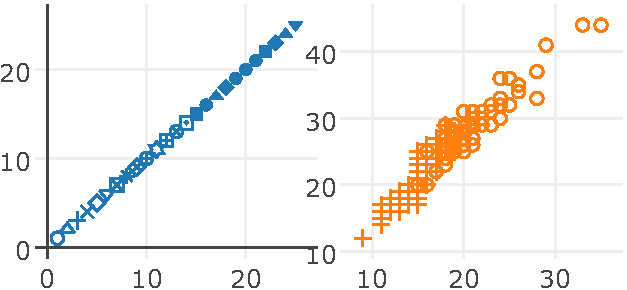
\includegraphics{bookdown_files/figure-latex/pch-1.pdf}
\caption{\label{fig:pch}Specifying symbol in a scatterplot}
\end{figure}

When mapping a numeric variable to \texttt{symbol}, it creates only one
trace, so no legend is generated. If you do want one trace per symbol,
make sure the variable you're mapping is a factor, as Figure
\ref{fig:symbol-factor} demonstrates. When plotting multiple traces, the
default plotly.js color scale will apply, but you can set the color of
every trace generated from this layer with
\texttt{color\ =\ I("black")}, or similar.

\begin{Shaded}
\begin{Highlighting}[]
\NormalTok{p <-}\StringTok{ }\KeywordTok{plot_ly}\NormalTok{(mpg, }\DataTypeTok{x =} \NormalTok{~cty, }\DataTypeTok{y =} \NormalTok{~hwy, }\DataTypeTok{alpha =} \FloatTok{0.3}\NormalTok{) }
\KeywordTok{subplot}\NormalTok{(}
  \KeywordTok{add_markers}\NormalTok{(p, }\DataTypeTok{symbol =} \NormalTok{~cyl, }\DataTypeTok{name =} \StringTok{"A single trace"}\NormalTok{),}
  \KeywordTok{add_markers}\NormalTok{(p, }\DataTypeTok{symbol =} \NormalTok{~}\KeywordTok{factor}\NormalTok{(cyl), }\DataTypeTok{color =} \KeywordTok{I}\NormalTok{(}\StringTok{"black"}\NormalTok{))}
\NormalTok{)}
\end{Highlighting}
\end{Shaded}

\begin{figure}[htbp]
\centering
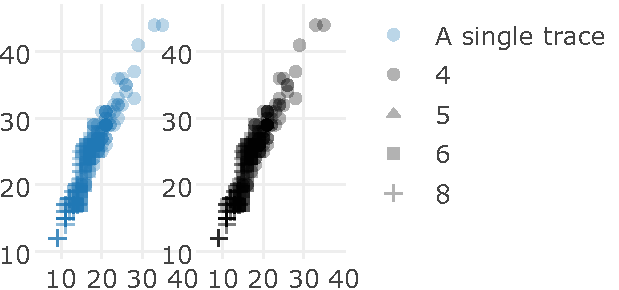
\includegraphics{bookdown_files/figure-latex/symbol-factor-1.pdf}
\caption{\label{fig:symbol-factor}Mapping symbol to a factor}
\end{figure}

The \texttt{color} argument adheres to similar rules as \texttt{symbol}:

\begin{itemize}
\item
  If numeric, \texttt{color} produces one trace, but
  \href{https://plot.ly/r/reference/\#scatter-marker-colorbar}{colorbar}
  is also generated to aide the decoding of colors back to data values.
  The \texttt{colorbar()} function can be used to customize the
  appearance of this automatically generated guide. The default
  colorscale is viridis, a perceptually-uniform colorscale (even when
  converted to black-and-white), and perceivable even to those with
  common forms of color blindness \citep{viridis}.
\item
  If discrete, \texttt{color} produces one trace per value, meaning a
  \href{https://plot.ly/r/reference/\#layout-legend}{legend} is
  generated. If an ordered factor, the default colorscale is viridis
  \citep{viridisLite}; otherwise, it is the ``Set2'' palette from the
  \textbf{RColorBrewer} package \citep{RColorBrewer}
\end{itemize}

\begin{Shaded}
\begin{Highlighting}[]
\NormalTok{p <-}\StringTok{ }\KeywordTok{plot_ly}\NormalTok{(mpg, }\DataTypeTok{x =} \NormalTok{~cty, }\DataTypeTok{y =} \NormalTok{~hwy, }\DataTypeTok{alpha =} \FloatTok{0.5}\NormalTok{)}
\KeywordTok{subplot}\NormalTok{(}
  \KeywordTok{add_markers}\NormalTok{(p, }\DataTypeTok{color =} \NormalTok{~cyl, }\DataTypeTok{showlegend =} \OtherTok{FALSE}\NormalTok{) %>%}\StringTok{ }
\StringTok{    }\KeywordTok{colorbar}\NormalTok{(}\DataTypeTok{title =} \StringTok{"Viridis"}\NormalTok{, }\DataTypeTok{len =} \DecValTok{1}\NormalTok{/}\DecValTok{2}\NormalTok{, }\DataTypeTok{y =} \DecValTok{1}\NormalTok{),}
  \KeywordTok{add_markers}\NormalTok{(p, }\DataTypeTok{color =} \NormalTok{~}\KeywordTok{factor}\NormalTok{(cyl))}
\NormalTok{) %>%}\StringTok{ }\KeywordTok{layout}\NormalTok{(}\DataTypeTok{showlegend =} \OtherTok{TRUE}\NormalTok{)}
\end{Highlighting}
\end{Shaded}

\begin{figure}[htbp]
\centering
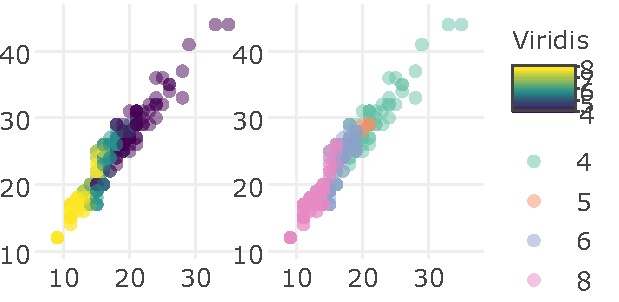
\includegraphics{bookdown_files/figure-latex/color-types-1.pdf}
\caption{\label{fig:color-types}Variations on a numeric color mapping.}
\end{figure}

There are a number of ways to alter the default colorscale via the
\texttt{colors} argument. This argument excepts: (1) a color brewer
palette name (see the row names of
\texttt{RColorBrewer::brewer.pal.info} for valid names), (2) a vector of
colors to interpolate, or (3) a color interpolation function like
\texttt{colorRamp()} or \texttt{scales::colour\_ramp()}. Although this
grants a lot of flexibility, one should be concious of using a
sequential colorscale for numeric variables (\& ordered factors) as
shown in \ref{fig:color-numeric}, and a qualitative colorscale for
discrete variables as shown in \ref{fig:color-discrete}. (TODO: touch on
lurking variables?)

\begin{Shaded}
\begin{Highlighting}[]
\KeywordTok{subplot}\NormalTok{(}
  \KeywordTok{add_markers}\NormalTok{(p, }\DataTypeTok{color =} \NormalTok{~cyl, }\DataTypeTok{colors =} \KeywordTok{c}\NormalTok{(}\StringTok{"#132B43"}\NormalTok{, }\StringTok{"#56B1F7"}\NormalTok{)) %>%}
\StringTok{    }\KeywordTok{colorbar}\NormalTok{(}\DataTypeTok{title =} \StringTok{"ggplot2 default"}\NormalTok{, }\DataTypeTok{len =} \DecValTok{1}\NormalTok{/}\DecValTok{3}\NormalTok{, }\DataTypeTok{y =} \DecValTok{1}\NormalTok{),}
  \KeywordTok{add_markers}\NormalTok{(p, }\DataTypeTok{color =} \NormalTok{~cyl, }\DataTypeTok{colors =} \NormalTok{viridisLite::}\KeywordTok{inferno}\NormalTok{(}\DecValTok{10}\NormalTok{)) %>%}\StringTok{ }
\StringTok{    }\KeywordTok{colorbar}\NormalTok{(}\DataTypeTok{title =} \StringTok{"Inferno"}\NormalTok{, }\DataTypeTok{len =} \DecValTok{1}\NormalTok{/}\DecValTok{3}\NormalTok{, }\DataTypeTok{y =} \DecValTok{2}\NormalTok{/}\DecValTok{3}\NormalTok{),}
  \KeywordTok{add_markers}\NormalTok{(p, }\DataTypeTok{color =} \NormalTok{~cyl, }\DataTypeTok{colors =} \KeywordTok{colorRamp}\NormalTok{(}\KeywordTok{c}\NormalTok{(}\StringTok{"red"}\NormalTok{, }\StringTok{"white"}\NormalTok{, }\StringTok{"blue"}\NormalTok{))) %>%}\StringTok{ }
\StringTok{    }\KeywordTok{colorbar}\NormalTok{(}\DataTypeTok{title =} \StringTok{"colorRamp"}\NormalTok{, }\DataTypeTok{len =} \DecValTok{1}\NormalTok{/}\DecValTok{3}\NormalTok{, }\DataTypeTok{y =} \DecValTok{1}\NormalTok{/}\DecValTok{3}\NormalTok{)}
\NormalTok{)}
\end{Highlighting}
\end{Shaded}

\begin{figure}[htbp]
\centering
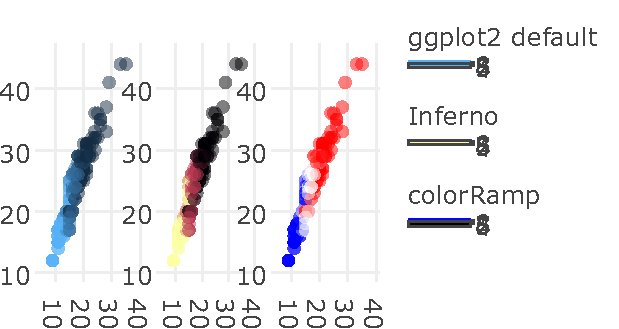
\includegraphics{bookdown_files/figure-latex/color-numeric-1.pdf}
\caption{\label{fig:color-numeric}Three variations on a numeric color
mapping}
\end{figure}

\begin{Shaded}
\begin{Highlighting}[]
\KeywordTok{subplot}\NormalTok{(}
  \KeywordTok{add_markers}\NormalTok{(p, }\DataTypeTok{color =} \NormalTok{~}\KeywordTok{factor}\NormalTok{(cyl), }\DataTypeTok{colors =} \StringTok{"Pastel1"}\NormalTok{),}
  \KeywordTok{add_markers}\NormalTok{(p, }\DataTypeTok{color =} \NormalTok{~}\KeywordTok{factor}\NormalTok{(cyl), }\DataTypeTok{colors =} \KeywordTok{colorRamp}\NormalTok{(}\KeywordTok{c}\NormalTok{(}\StringTok{"red"}\NormalTok{, }\StringTok{"blue"}\NormalTok{))),}
  \KeywordTok{add_markers}\NormalTok{(p, }\DataTypeTok{color =} \NormalTok{~}\KeywordTok{factor}\NormalTok{(cyl), }
              \DataTypeTok{colors =} \KeywordTok{c}\NormalTok{(}\StringTok{`}\DataTypeTok{4}\StringTok{`} \NormalTok{=}\StringTok{ "red"}\NormalTok{, }\StringTok{`}\DataTypeTok{5}\StringTok{`} \NormalTok{=}\StringTok{ "black"}\NormalTok{, }\StringTok{`}\DataTypeTok{6}\StringTok{`} \NormalTok{=}\StringTok{ "blue"}\NormalTok{, }\StringTok{`}\DataTypeTok{8}\StringTok{`} \NormalTok{=}\StringTok{ "green"}\NormalTok{))}
\NormalTok{) %>%}\StringTok{ }\KeywordTok{layout}\NormalTok{(}\DataTypeTok{showlegend =} \OtherTok{FALSE}\NormalTok{)}
\end{Highlighting}
\end{Shaded}

\begin{figure}[htbp]
\centering
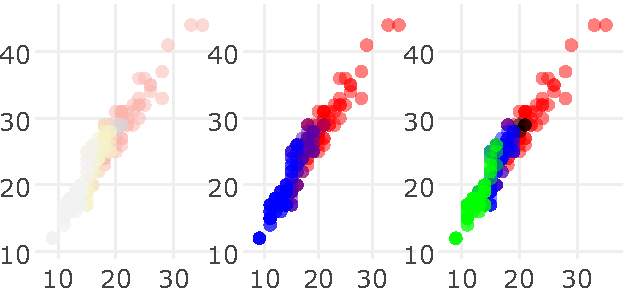
\includegraphics{bookdown_files/figure-latex/color-discrete-1.pdf}
\caption{\label{fig:color-discrete}Three variations on a discrete color
mapping}
\end{figure}

For scatterplots, the \texttt{size} argument controls the area of
markers (unless otherwise specified via
\href{https://plot.ly/r/reference/\#scatter-marker-sizemode}{sizemode}),
and \emph{must} be a numeric variable. The \texttt{sizes} argument
controls the minimum and maximum size of circles, in pixels:

\begin{Shaded}
\begin{Highlighting}[]
\KeywordTok{subplot}\NormalTok{(}
  \KeywordTok{add_markers}\NormalTok{(p, }\DataTypeTok{size =} \NormalTok{~cyl, }\DataTypeTok{name =} \StringTok{"default"}\NormalTok{),}
  \KeywordTok{add_markers}\NormalTok{(p, }\DataTypeTok{size =} \NormalTok{~cyl, }\DataTypeTok{sizes =} \KeywordTok{c}\NormalTok{(}\DecValTok{1}\NormalTok{, }\DecValTok{500}\NormalTok{), }\DataTypeTok{name =} \StringTok{"custom"}\NormalTok{)}
\NormalTok{)}
\end{Highlighting}
\end{Shaded}

\begin{figure}[htbp]
\centering
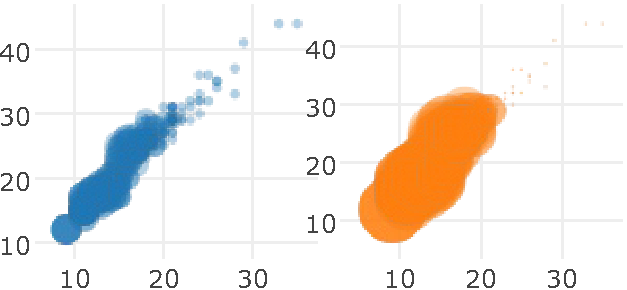
\includegraphics{bookdown_files/figure-latex/unnamed-chunk-21-1.pdf}
\caption{}
\end{figure}

\subsubsection{3D scatterplots}\label{d-scatterplots}

To make a 3D scatterplot, just add a \texttt{z} attribute:

\begin{Shaded}
\begin{Highlighting}[]
\KeywordTok{plot_ly}\NormalTok{(mpg, }\DataTypeTok{x =} \NormalTok{~cty, }\DataTypeTok{y =} \NormalTok{~hwy, }\DataTypeTok{z =} \NormalTok{~cyl) %>%}
\StringTok{  }\KeywordTok{add_markers}\NormalTok{(}\DataTypeTok{color =} \NormalTok{~cyl)}
\end{Highlighting}
\end{Shaded}

\begin{figure}[htbp]
\centering

\includegraphics{bookdown_files/figure-latex/3D-scatterplot-1.pdf}
\caption{\label{fig:3D-scatterplot}A 3D scatterplot}
\end{figure}

\subsubsection{Scatterplot matrices}\label{scatterplot-matrices}

Scatterplot matrices \emph{can} be made via \texttt{plot\_ly()} and
\texttt{subplot()}, but \texttt{ggplotly()} has a special method for
translating ggmatrix objects from the \textbf{GGally} package to plotly
objects \citep{GGally}. These objects are essentially a matrix of ggplot
objects and are the underlying data structure which powers higher level
functions in \textbf{GGally}, such as \texttt{ggpairs()}, a function for
creating a generalized pairs plot \citep{gpp}. The generalized pairs
plot could be motivated as a generalization of the scatterplot matrix
which supports categorical data and different visual representations of
the data beyond a scatterplot. Figure \ref{fig:ggpairs} shows an
interactive version of the generalized pairs plot made via
\texttt{ggpairs()} and \texttt{ggplotly()}. In
\protect\hyperlink{linking-views-without-shiny}{Linking views without
shiny}, we explore how this framework can be extended to enable linked
brushing in the generalized pairs plot.

\begin{Shaded}
\begin{Highlighting}[]
\NormalTok{pm <-}\StringTok{ }\NormalTok{GGally::}\KeywordTok{ggpairs}\NormalTok{(iris)}
\KeywordTok{ggplotly}\NormalTok{(pm)}
\end{Highlighting}
\end{Shaded}

\begin{figure}[htbp]
\centering
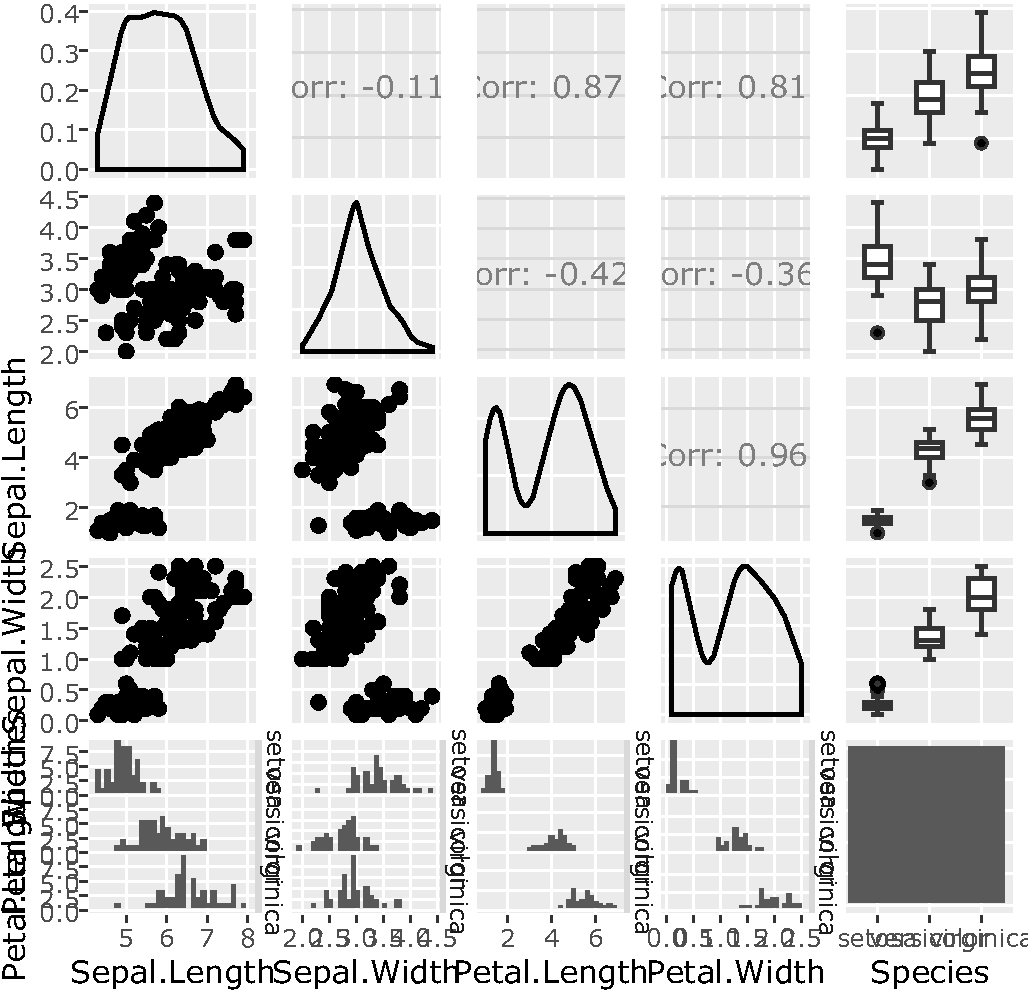
\includegraphics{bookdown_files/figure-latex/ggpairs-1.pdf}
\caption{\label{fig:ggpairs}An interactive version of the generalized pairs
plot made via the \texttt{ggpairs()} function from the \textbf{GGally}
package}
\end{figure}

\subsection{Dotplots \& error bars}\label{dotplots-error-bars}

A dotplot is similar to a scatterplot, except instead of two numeric
axes, one is categorical. The usual goal of a dotplot is to compare
value(s) on a numerical scale over numerous categories. In this context,
dotplots are preferrable to pie charts since comparing position along a
common scale is much easier than comparing angle or area
\citep{graphical-perception};
\citep{crowdsourcing-graphical-perception}. Furthermore, dotplots can be
preferrable to bar charts, especially when comparing values within a
narrow range far away from 0 \citep{few-values}. Also, when presenting
point estimates, and uncertainty associated with those estimates, bar
charts tend to exaggerate the difference in point estimates, and lose
focus on uncertainty \citep{messing}.

A popular application for dotplots (with error bars) is the so-called
``coefficient plot'' for visualizing the point estimates of coefficients
and their standard error. The \texttt{coefplot()} function in the
\textbf{coefplot} package \citep{coefplot} and the \texttt{ggcoef()}
function in the \textbf{GGally} both produce coefficient plots for many
types of model objects in R using \textbf{ggplot2}, which we can
translate to plotly via \texttt{ggplotly()}. Since these packages use
points and segments to draw the coefficient plots, the hover information
is not the best, and it'd be better to use
\href{https://plot.ly/r/reference/\#scatter-error_x}{error objects}.
Figure \ref{fig:coefplot} uses the \texttt{tidy()} function from the
\textbf{broom} package \citep{broom} to obtain a data frame with one row
per model coefficient, and produce a coefficient plot with error bars
along the x-axis.

\begin{Shaded}
\begin{Highlighting}[]
\NormalTok{m <-}\StringTok{ }\KeywordTok{lm}\NormalTok{(Sepal.Length ~}\StringTok{ }\NormalTok{Sepal.Width *}\StringTok{ }\NormalTok{Petal.Length *}\StringTok{ }\NormalTok{Petal.Width, }\DataTypeTok{data =} \NormalTok{iris)}
\CommentTok{# arrange by estimate, then make term a factor to order categories in the plot}
\NormalTok{d <-}\StringTok{ }\NormalTok{broom::}\KeywordTok{tidy}\NormalTok{(m) %>%}\StringTok{ }
\StringTok{  }\KeywordTok{arrange}\NormalTok{(}\KeywordTok{desc}\NormalTok{(estimate)) %>%}
\StringTok{  }\KeywordTok{mutate}\NormalTok{(}\DataTypeTok{term =} \KeywordTok{factor}\NormalTok{(term, }\DataTypeTok{levels =} \NormalTok{term))}
\KeywordTok{plot_ly}\NormalTok{(d, }\DataTypeTok{x =} \NormalTok{~estimate, }\DataTypeTok{y =} \NormalTok{~term) %>%}
\StringTok{  }\KeywordTok{add_markers}\NormalTok{(}\DataTypeTok{error_x =} \NormalTok{~}\KeywordTok{list}\NormalTok{(}\DataTypeTok{value =} \NormalTok{std.error)) %>%}
\StringTok{  }\KeywordTok{layout}\NormalTok{(}\DataTypeTok{margin =} \KeywordTok{list}\NormalTok{(}\DataTypeTok{l =} \DecValTok{200}\NormalTok{))}
\end{Highlighting}
\end{Shaded}

\begin{figure}[htbp]
\centering
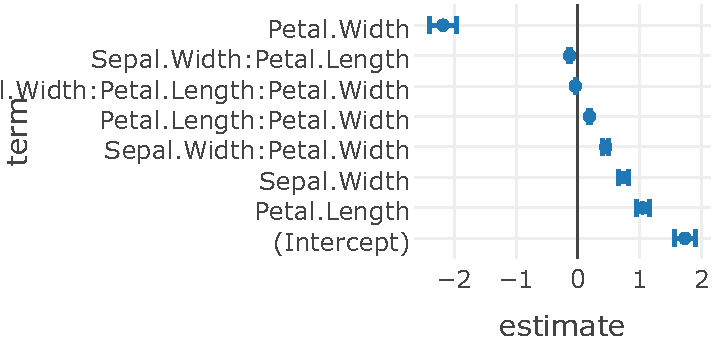
\includegraphics{bookdown_files/figure-latex/coefplot-1.pdf}
\caption{\label{fig:coefplot}A coefficient plot}
\end{figure}

\hypertarget{line-plots}{\subsection{Line plots}\label{line-plots}}

This section surveys useful applications of \texttt{add\_lines()} and
\texttt{add\_paths()}. The only difference between these functions is
that \texttt{add\_lines()} connects x/y pairs from left to right,
instead of the order in which the data appears. Both functions
understand the \texttt{color}, \texttt{linetype}, and \texttt{alpha}
attributes\footnote{plotly.js currently
  \href{https://github.com/plotly/plotly.js/issues/147}{does not support
  data arrays for \texttt{scatter.line.width} or
  \texttt{scatter.line.color}}, meaning a single line trace can only
  have one width/color in 2D line plot, and consequently numeric
  \texttt{color}/\texttt{size} mappings won't work}, as well as
groupings defined by \texttt{group\_by()}.

Figure \ref{fig:houston} uses \texttt{group\_by()} to plot one line per
city in the \texttt{txhousing} dataset using a \emph{single} trace.
Since there can only be one tooltip per trace, hovering over that plot
does not reveal useful information. Although plotting many traces can be
computationally expensive, it is necessary in order to display better
information on hover. Since the \texttt{color} argument produces one
trace per value (if the variable (\texttt{city}) is discrete), hovering
on Figure \ref{fig:many-traces} reveals the top \textasciitilde{}10
cities at a given x value. Since 46 colors is too many to perceive in a
single plot, Figure \ref{fig:many-traces} also restricts the set of
possible \texttt{colors} to black.

\begin{Shaded}
\begin{Highlighting}[]
\KeywordTok{plot_ly}\NormalTok{(txhousing, }\DataTypeTok{x =} \NormalTok{~date, }\DataTypeTok{y =} \NormalTok{~median) %>%}
\StringTok{  }\KeywordTok{add_lines}\NormalTok{(}\DataTypeTok{color =} \NormalTok{~city, }\DataTypeTok{colors =} \StringTok{"black"}\NormalTok{, }\DataTypeTok{alpha =} \FloatTok{0.2}\NormalTok{)}
\end{Highlighting}
\end{Shaded}

\begin{figure}[htbp]
\centering
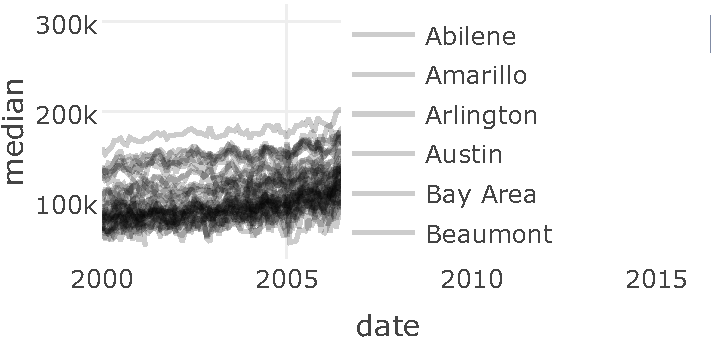
\includegraphics{bookdown_files/figure-latex/many-traces-1.pdf}
\caption{\label{fig:many-traces}Median house sales with one trace per city.}
\end{figure}

Generally speaking, it's hard to perceive more than 8 different
colors/linetypes/symbols in a given plot, so sometimes we have to filter
data to use these effectively. Here we use the \textbf{dplyr} package to
find the top 5 cities in terms of average monthly sales (\texttt{top5}),
then effectively filter the original data to contain just these cities
via \texttt{semi\_join()}. Once we have the data is filtered, mapping
city to \texttt{color} or \texttt{linetype} is trivial. The color
palette can be altered via the \texttt{colors} argument, and follows the
same rules as \protect\hyperlink{scatterplots}{scatterplots}. The
linetype palette can be altered via the \texttt{linetypes} argument, and
accepts R's
\href{https://github.com/wch/r-source/blob/e5b21d0397c607883ff25cca379687b86933d730/src/library/graphics/man/par.Rd\#L726-L743}{\texttt{lty}
values} or plotly.js
\href{https://plot.ly/r/reference/\#scatter-line-dash}{dash values}.

\begin{Shaded}
\begin{Highlighting}[]
\KeywordTok{library}\NormalTok{(dplyr)}
\NormalTok{top5 <-}\StringTok{ }\NormalTok{txhousing %>%}
\StringTok{  }\KeywordTok{group_by}\NormalTok{(city) %>%}
\StringTok{  }\KeywordTok{summarise}\NormalTok{(}\DataTypeTok{m =} \KeywordTok{mean}\NormalTok{(sales, }\DataTypeTok{na.rm =} \OtherTok{TRUE}\NormalTok{)) %>%}
\StringTok{  }\KeywordTok{arrange}\NormalTok{(}\KeywordTok{desc}\NormalTok{(m)) %>%}
\StringTok{  }\KeywordTok{top_n}\NormalTok{(}\DecValTok{5}\NormalTok{)}

\NormalTok{p <-}\StringTok{ }\KeywordTok{semi_join}\NormalTok{(txhousing, top5) %>%}
\StringTok{  }\KeywordTok{plot_ly}\NormalTok{(}\DataTypeTok{x =} \NormalTok{~date, }\DataTypeTok{y =} \NormalTok{~median)}

\KeywordTok{subplot}\NormalTok{(}
  \KeywordTok{add_lines}\NormalTok{(p, }\DataTypeTok{color =} \NormalTok{~city),}
  \KeywordTok{add_lines}\NormalTok{(p, }\DataTypeTok{linetype =} \NormalTok{~city),}
  \DataTypeTok{shareX =} \OtherTok{TRUE}\NormalTok{, }\DataTypeTok{nrows =} \DecValTok{2}
\NormalTok{)}
\end{Highlighting}
\end{Shaded}

\begin{figure}[htbp]
\centering
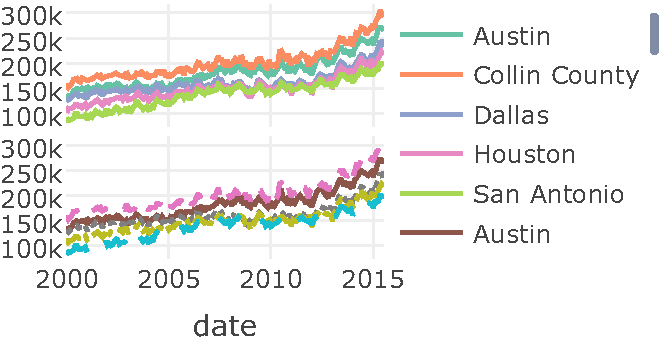
\includegraphics{bookdown_files/figure-latex/unnamed-chunk-22-1.pdf}
\caption{}
\end{figure}

\subsubsection{Density plots}\label{density-plots}

In \protect\hyperlink{bars-histograms}{Bars \& histograms}, we leveraged
a number of algorithms in R for computing the ``optimal'' number of bins
for a histogram, via \texttt{hist()}, and routing those results to
\texttt{add\_bars()}.

\begin{Shaded}
\begin{Highlighting}[]
\NormalTok{kerns <-}\StringTok{ }\KeywordTok{c}\NormalTok{(}\StringTok{"gaussian"}\NormalTok{, }\StringTok{"epanechnikov"}\NormalTok{, }\StringTok{"rectangular"}\NormalTok{, }
          \StringTok{"triangular"}\NormalTok{, }\StringTok{"biweight"}\NormalTok{, }\StringTok{"cosine"}\NormalTok{, }\StringTok{"optcosine"}\NormalTok{)}
\NormalTok{p <-}\StringTok{ }\KeywordTok{plot_ly}\NormalTok{()}
\NormalTok{for (k in kerns) \{}
  \NormalTok{d <-}\StringTok{ }\KeywordTok{density}\NormalTok{(txhousing$median, }\DataTypeTok{kernel =} \NormalTok{k, }\DataTypeTok{na.rm =} \OtherTok{TRUE}\NormalTok{)}
  \NormalTok{p <-}\StringTok{ }\KeywordTok{add_lines}\NormalTok{(p, }\DataTypeTok{x =} \NormalTok{d$x, }\DataTypeTok{y =} \NormalTok{d$y, }\DataTypeTok{name =} \NormalTok{k)}
\NormalTok{\}}
\KeywordTok{layout}\NormalTok{(p, }\DataTypeTok{xaxis =} \KeywordTok{list}\NormalTok{(}\DataTypeTok{title =} \StringTok{"Median monthly price"}\NormalTok{))}
\end{Highlighting}
\end{Shaded}

\begin{figure}[htbp]
\centering
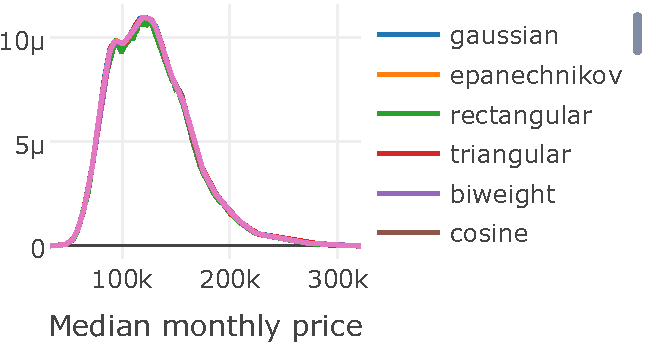
\includegraphics{bookdown_files/figure-latex/unnamed-chunk-23-1.pdf}
\caption{}
\end{figure}

\subsubsection{Parallel Coordinates}\label{parallel-coordinates}

One very useful, but often overlooked, visualization technique is the
parallel coordinates plot. Parallel coordinates provide a way to compare
values along a common (or non-aligned) positional scale(s) -- the most
basic of all perceptual tasks -- in more than 3 dimensions
\citep{graphical-perception}. Usually each line represents every
measurement for a given row (or observation) in a data set. When
measurements are on very different scales, some care must be taken, and
variables must transformed to be put on a common scale. As Figure
\ref{fig:pcp-common} shows, even when variables are measured on a
similar scale, it can still be a informative to transform variables in
different ways.

\begin{Shaded}
\begin{Highlighting}[]
\NormalTok{iris$obs <-}\StringTok{ }\KeywordTok{seq_len}\NormalTok{(}\KeywordTok{nrow}\NormalTok{(iris))}
\NormalTok{iris_pcp <-}\StringTok{ }\NormalTok{function(}\DataTypeTok{transform =} \NormalTok{identity) \{}
  \NormalTok{iris[] <-}\StringTok{ }\NormalTok{purrr::}\KeywordTok{map_if}\NormalTok{(iris, is.numeric, transform)}
  \NormalTok{tidyr::}\KeywordTok{gather}\NormalTok{(iris, variable, value, -Species, -obs) %>%}\StringTok{ }
\StringTok{    }\KeywordTok{group_by}\NormalTok{(obs) %>%}\StringTok{ }
\StringTok{    }\KeywordTok{plot_ly}\NormalTok{(}\DataTypeTok{x =} \NormalTok{~variable, }\DataTypeTok{y =} \NormalTok{~value, }\DataTypeTok{color =} \NormalTok{~Species) %>%}\StringTok{ }
\StringTok{    }\KeywordTok{add_lines}\NormalTok{(}\DataTypeTok{alpha =} \FloatTok{0.3}\NormalTok{)}
\NormalTok{\}}
\KeywordTok{subplot}\NormalTok{(}
  \KeywordTok{iris_pcp}\NormalTok{(), }
  \KeywordTok{iris_pcp}\NormalTok{(scale),}
  \KeywordTok{iris_pcp}\NormalTok{(scales::rescale)}
\NormalTok{) %>%}\StringTok{ }\KeywordTok{hide_legend}\NormalTok{()}
\end{Highlighting}
\end{Shaded}

\begin{figure}[htbp]
\centering
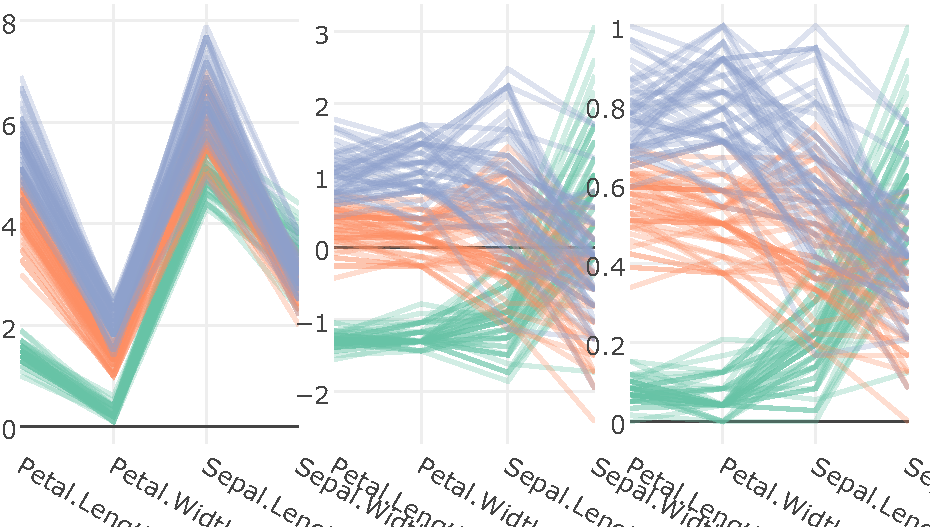
\includegraphics{bookdown_files/figure-latex/pcp-common-1.pdf}
\caption{\label{fig:pcp-common}Parallel coordinates plots of the Iris
dataset. On the left is the raw measurements. In the middle, each
variable is scaled to have mean of 0 and standard deviation of 1. On the
right, each variable is scaled to have a minimum of 0 and a maximum of
1.}
\end{figure}

It is also worth noting that the \textbf{GGally} offers a
\texttt{ggparcoord()} function which creates parallel coordinate plots
via \textbf{ggplot2}, which we can convert to plotly via
\texttt{ggplotly()}. In \protect\hyperlink{linked-highlighting}{linked
highlighting}, parallel coordinates are linked to lower dimensional (but
sometimes higher resolution) graphics of related data to guide
multi-variate data exploration.

\subsubsection{3D line plots}\label{d-line-plots}

To make a 3D line plot, just add a \texttt{z} attribute (in addition to
\texttt{x} and \texttt{y}):

\begin{Shaded}
\begin{Highlighting}[]
\KeywordTok{plot_ly}\NormalTok{(mpg, }\DataTypeTok{x =} \NormalTok{~cty, }\DataTypeTok{y =} \NormalTok{~hwy, }\DataTypeTok{z =} \NormalTok{~cyl) %>%}
\StringTok{  }\KeywordTok{add_lines}\NormalTok{(}\DataTypeTok{color =} \NormalTok{~displ)}
\end{Highlighting}
\end{Shaded}

\begin{figure}[htbp]
\centering

\includegraphics{bookdown_files/figure-latex/3D-lines-1.pdf}
\caption{\label{fig:3D-lines}A 3D scatterplot}
\end{figure}

\subsection{Segments}\label{segments}

The \texttt{add\_segments()} function essentially provides a way to
connect two points ((\texttt{x}, \texttt{y}) to (\texttt{xend},
\texttt{yend})) with a line. Segments form the building blocks for many
useful chart types, including candlestick charts, a popular way to
visualize stock prices. Figure \ref{fig:candlestick} uses the
\textbf{quantmod} package \citep{quantmod} to obtain stock price data
for Microsoft and plots two segments for each day: one to encode the
opening/closing values, and one to encode the daily high/low.

\begin{Shaded}
\begin{Highlighting}[]
\KeywordTok{library}\NormalTok{(quantmod)}
\NormalTok{msft <-}\StringTok{ }\KeywordTok{getSymbols}\NormalTok{(}\StringTok{"MSFT"}\NormalTok{, }\DataTypeTok{auto.assign =} \NormalTok{F)}
\NormalTok{dat <-}\StringTok{ }\KeywordTok{as.data.frame}\NormalTok{(msft)}
\NormalTok{dat$date <-}\StringTok{ }\KeywordTok{index}\NormalTok{(msft)}
\NormalTok{dat <-}\StringTok{ }\KeywordTok{subset}\NormalTok{(dat, date >=}\StringTok{ "2016-01-01"}\NormalTok{)}

\KeywordTok{names}\NormalTok{(dat) <-}\StringTok{ }\KeywordTok{sub}\NormalTok{(}\StringTok{"^MSFT}\CharTok{\textbackslash{}\textbackslash{}}\StringTok{."}\NormalTok{, }\StringTok{""}\NormalTok{, }\KeywordTok{names}\NormalTok{(dat))}

\KeywordTok{plot_ly}\NormalTok{(dat, }\DataTypeTok{x =} \NormalTok{~date, }\DataTypeTok{xend =} \NormalTok{~date, }\DataTypeTok{color =} \NormalTok{~Close >}\StringTok{ }\NormalTok{Open, }
        \DataTypeTok{colors =} \KeywordTok{c}\NormalTok{(}\StringTok{"red"}\NormalTok{, }\StringTok{"forestgreen"}\NormalTok{), }\DataTypeTok{hoverinfo =} \StringTok{"none"}\NormalTok{) %>%}
\StringTok{  }\KeywordTok{add_segments}\NormalTok{(}\DataTypeTok{y =} \NormalTok{~Low, }\DataTypeTok{yend =} \NormalTok{~High, }\DataTypeTok{size =} \KeywordTok{I}\NormalTok{(}\DecValTok{1}\NormalTok{)) %>%}
\StringTok{  }\KeywordTok{add_segments}\NormalTok{(}\DataTypeTok{y =} \NormalTok{~Open, }\DataTypeTok{yend =} \NormalTok{~Close, }\DataTypeTok{size =} \KeywordTok{I}\NormalTok{(}\DecValTok{3}\NormalTok{)) %>%}
\StringTok{  }\KeywordTok{layout}\NormalTok{(}\DataTypeTok{showlegend =} \OtherTok{FALSE}\NormalTok{, }\DataTypeTok{yaxis =} \KeywordTok{list}\NormalTok{(}\DataTypeTok{title =} \StringTok{"Price"}\NormalTok{)) %>%}
\StringTok{  }\KeywordTok{rangeslider}\NormalTok{()}
\end{Highlighting}
\end{Shaded}

\begin{figure}[htbp]
\centering
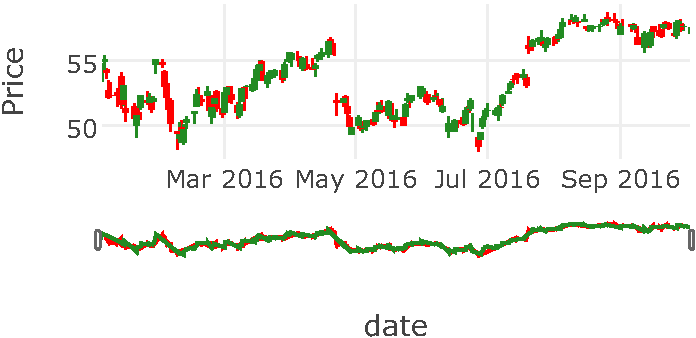
\includegraphics{bookdown_files/figure-latex/candlestick-1.pdf}
\caption{\label{fig:candlestick}A candelstick chart}
\end{figure}

\subsection{Ribbons}\label{ribbons}

Ribbons are useful for showing uncertainy bounds as a function of x. The
\texttt{add\_ribbons()} function creates ribbons and requires the
arguments: \texttt{ymin} and \texttt{ymax}. The \texttt{augment()}
function from the \textbf{broom} package appends observational-level
model components (e.g., fitted values stored as a new column
\texttt{.fitted}) which is useful for extracting those components in a
form that is convenient for visualization.

\begin{Shaded}
\begin{Highlighting}[]
\NormalTok{m <-}\StringTok{ }\KeywordTok{lm}\NormalTok{(mpg ~}\StringTok{ }\NormalTok{wt, }\DataTypeTok{data =} \NormalTok{mtcars)}
\NormalTok{broom::}\KeywordTok{augment}\NormalTok{(m) %>%}
\StringTok{  }\KeywordTok{plot_ly}\NormalTok{(}\DataTypeTok{x =} \NormalTok{~wt, }\DataTypeTok{showlegend =} \OtherTok{FALSE}\NormalTok{) %>%}
\StringTok{  }\KeywordTok{add_markers}\NormalTok{(}\DataTypeTok{y =} \NormalTok{~mpg, }\DataTypeTok{color =} \KeywordTok{I}\NormalTok{(}\StringTok{"black"}\NormalTok{)) %>%}
\StringTok{  }\KeywordTok{add_ribbons}\NormalTok{(}\DataTypeTok{ymin =} \NormalTok{~.fitted -}\StringTok{ }\FloatTok{1.96} \NormalTok{*}\StringTok{ }\NormalTok{.se.fit, }
              \DataTypeTok{ymax =} \NormalTok{~.fitted +}\StringTok{ }\FloatTok{1.96} \NormalTok{*}\StringTok{ }\NormalTok{.se.fit, }\DataTypeTok{color =} \KeywordTok{I}\NormalTok{(}\StringTok{"gray80"}\NormalTok{)) %>%}
\StringTok{  }\KeywordTok{add_lines}\NormalTok{(}\DataTypeTok{y =} \NormalTok{~.fitted, }\DataTypeTok{color =} \KeywordTok{I}\NormalTok{(}\StringTok{"steelblue"}\NormalTok{))}
\end{Highlighting}
\end{Shaded}

\begin{figure}[htbp]
\centering
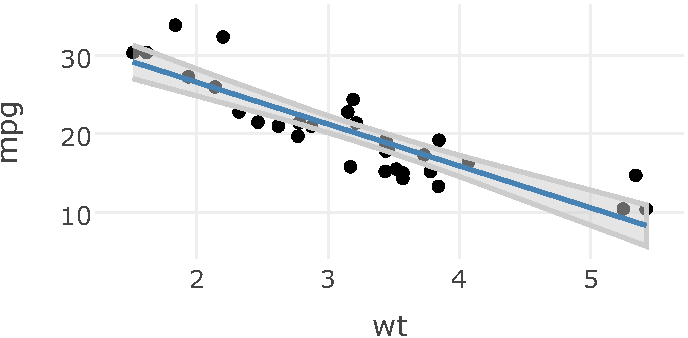
\includegraphics{bookdown_files/figure-latex/unnamed-chunk-25-1.pdf}
\caption{}
\end{figure}

\hypertarget{polygons}{\subsection{Polygons}\label{polygons}}

The \texttt{add\_polygons()} function is essentially equivalent to
\texttt{add\_paths()} with the
\href{https://plot.ly/r/reference/\#scatter-fill}{fill} attribute set to
``toself''. Polygons from the basis for other, higher-level, geometries
such as \texttt{add\_ribbons()}, but can be useful in their own right.

\begin{Shaded}
\begin{Highlighting}[]
\KeywordTok{map_data}\NormalTok{(}\StringTok{"world"}\NormalTok{, }\StringTok{"canada"}\NormalTok{) %>%}
\StringTok{  }\KeywordTok{group_by}\NormalTok{(group) %>%}
\StringTok{  }\KeywordTok{plot_ly}\NormalTok{(}\DataTypeTok{x =} \NormalTok{~long, }\DataTypeTok{y =} \NormalTok{~lat, }\DataTypeTok{alpha =} \FloatTok{0.2}\NormalTok{) %>%}
\StringTok{  }\KeywordTok{add_polygons}\NormalTok{(}\DataTypeTok{hoverinfo =} \StringTok{"none"}\NormalTok{, }\DataTypeTok{color =} \KeywordTok{I}\NormalTok{(}\StringTok{"black"}\NormalTok{)) %>%}
\StringTok{  }\KeywordTok{add_markers}\NormalTok{(}\DataTypeTok{text =} \NormalTok{~}\KeywordTok{paste}\NormalTok{(name, }\StringTok{"<br />"}\NormalTok{, pop), }\DataTypeTok{hoverinfo =} \StringTok{"text"}\NormalTok{, }
              \DataTypeTok{color =} \KeywordTok{I}\NormalTok{(}\StringTok{"red"}\NormalTok{), }\DataTypeTok{data =} \NormalTok{maps::canada.cities) %>%}
\StringTok{  }\KeywordTok{layout}\NormalTok{(}\DataTypeTok{showlegend =} \OtherTok{FALSE}\NormalTok{)}
\end{Highlighting}
\end{Shaded}

{[}{]}(bookdown\_files/figure-latex/map-canada, ``A map of Canada using
the default cartesian coordinate system.''-1.pdf)

\section{Maps}\label{maps}

\subsection{Using scatter traces}\label{using-scatter-traces}

As shown in \protect\hyperlink{polygons}{polygons}, it is possible to
create maps using plotly's default (cartesian) coordinate system, but
plotly.js also has support for plotting
\protect\hyperlink{scatter-traces}{scatter traces} on top of either a
\href{https://plot.ly/r/reference/\#layout-geo}{custom geo layout} or a
\href{https://plot.ly/r/reference/\#layout-mapbox}{mapbox layout}.
Figure \ref{fig:maps} compares the three different layout options in a
single subplot.

\begin{Shaded}
\begin{Highlighting}[]
\NormalTok{dat <-}\StringTok{ }\KeywordTok{map_data}\NormalTok{(}\StringTok{"world"}\NormalTok{, }\StringTok{"canada"}\NormalTok{) %>%}\StringTok{ }\KeywordTok{group_by}\NormalTok{(group)}

\NormalTok{map1 <-}\StringTok{ }\KeywordTok{plot_ly}\NormalTok{(dat, }\DataTypeTok{x =} \NormalTok{~long, }\DataTypeTok{y =} \NormalTok{~lat) %>%}\StringTok{ }
\StringTok{  }\KeywordTok{add_paths}\NormalTok{(}\DataTypeTok{size =} \KeywordTok{I}\NormalTok{(}\DecValTok{1}\NormalTok{)) %>%}
\StringTok{  }\KeywordTok{add_segments}\NormalTok{(}\DataTypeTok{x =} \NormalTok{-}\DecValTok{100}\NormalTok{, }\DataTypeTok{xend =} \NormalTok{-}\DecValTok{50}\NormalTok{, }\DataTypeTok{y =} \DecValTok{50}\NormalTok{, }\DecValTok{75}\NormalTok{)}

\NormalTok{map2 <-}\StringTok{ }\KeywordTok{plot_mapbox}\NormalTok{(dat, }\DataTypeTok{x =} \NormalTok{~long, }\DataTypeTok{y =} \NormalTok{~lat) %>%}\StringTok{ }
\StringTok{  }\KeywordTok{add_paths}\NormalTok{(}\DataTypeTok{size =} \KeywordTok{I}\NormalTok{(}\DecValTok{2}\NormalTok{)) %>%}
\StringTok{  }\KeywordTok{add_segments}\NormalTok{(}\DataTypeTok{x =} \NormalTok{-}\DecValTok{100}\NormalTok{, }\DataTypeTok{xend =} \NormalTok{-}\DecValTok{50}\NormalTok{, }\DataTypeTok{y =} \DecValTok{50}\NormalTok{, }\DecValTok{75}\NormalTok{) %>%}
\StringTok{  }\KeywordTok{layout}\NormalTok{(}\DataTypeTok{mapbox =} \KeywordTok{list}\NormalTok{(}\DataTypeTok{zoom =} \DecValTok{0}\NormalTok{,}
      \DataTypeTok{center =} \KeywordTok{list}\NormalTok{(}\DataTypeTok{lat =} \NormalTok{~}\KeywordTok{median}\NormalTok{(lat), }\DataTypeTok{lon =} \NormalTok{~}\KeywordTok{median}\NormalTok{(long))}
   \NormalTok{))}

\CommentTok{# geo() is the only object type which supports different map projections}
\NormalTok{map3 <-}\StringTok{ }\KeywordTok{plot_geo}\NormalTok{(dat, }\DataTypeTok{x =} \NormalTok{~long, }\DataTypeTok{y =} \NormalTok{~lat) %>%}\StringTok{ }
\StringTok{  }\KeywordTok{add_markers}\NormalTok{(}\DataTypeTok{size =} \KeywordTok{I}\NormalTok{(}\DecValTok{1}\NormalTok{)) %>%}
\StringTok{  }\KeywordTok{add_segments}\NormalTok{(}\DataTypeTok{x =} \NormalTok{-}\DecValTok{100}\NormalTok{, }\DataTypeTok{xend =} \NormalTok{-}\DecValTok{50}\NormalTok{, }\DataTypeTok{y =} \DecValTok{50}\NormalTok{, }\DecValTok{75}\NormalTok{) %>%}
\StringTok{  }\KeywordTok{layout}\NormalTok{(}\DataTypeTok{geo =} \KeywordTok{list}\NormalTok{(}\DataTypeTok{projection =} \KeywordTok{list}\NormalTok{(}\DataTypeTok{type =} \StringTok{"mercator"}\NormalTok{)))}

\KeywordTok{subplot}\NormalTok{(map1, map2) %>%}
\StringTok{  }\KeywordTok{subplot}\NormalTok{(map3, }\DataTypeTok{nrows =} \DecValTok{2}\NormalTok{) %>%}\StringTok{ }
\StringTok{  }\KeywordTok{hide_legend}\NormalTok{()}
\end{Highlighting}
\end{Shaded}

\begin{figure}[htbp]
\centering
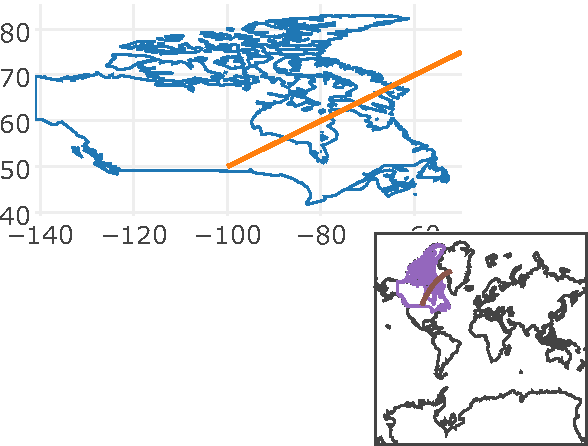
\includegraphics{bookdown_files/figure-latex/maps-1.pdf}
\caption{\label{fig:maps}A few maps}
\end{figure}

Any of the \texttt{add\_*()} functions found under
\href{https://cpsievert.github.io/plotly_book/scatter-traces.html}{scatter
traces} should work as expected on plotly-geo (initialized via
\texttt{plot\_geo()}) or plotly-mapbox (initialized via
\texttt{plot\_mapbox()}) objects. You can think of \texttt{plot\_geo()}
and \texttt{plot\_mapbox()} as special cases (or more opiniated
versions) of \texttt{plot\_ly()}. For one, they won't allow you to mix
scatter and non-scatter traces in a single plot object, which you
probably don't want to do anyway. In order to enable Figure
\ref{fig:maps}, plotly.js \emph{can't} make this restriction, but since
we have \texttt{subplot()} in R, we \emph{can} make this restriction
without sacrificing flexibility.

\subsection{Choropleths}\label{choropleths}

In addition to scatter traces, plotly-geo objects can also create a
\href{https://plot.ly/r/reference/\#choropleth}{choropleth} trace/layer.
Figure \ref{fig:us-density} shows the population density of the U.S. via
a choropleth, and also layers on markers for the state center locations,
using the U.S. state data from the \textbf{datasets} package
\citep{base}. By simply providing a
\href{https://plot.ly/r/reference/\#choropleth-z}{\texttt{z}} attribute,
plotly-geo objects will try to create a choropleth, but you'll also need
to provide
\href{https://plot.ly/r/reference/\#choropleth-locations}{\texttt{locations}}
and a
\href{https://plot.ly/r/reference/\#choropleth-locationmode}{\texttt{locationmode}}.

\begin{Shaded}
\begin{Highlighting}[]
\NormalTok{density <-}\StringTok{ }\NormalTok{state.x77[, }\StringTok{"Population"}\NormalTok{] /}\StringTok{ }\NormalTok{state.x77[, }\StringTok{"Area"}\NormalTok{]}

\NormalTok{g <-}\StringTok{ }\KeywordTok{list}\NormalTok{(}
  \DataTypeTok{scope =} \StringTok{'usa'}\NormalTok{,}
  \DataTypeTok{projection =} \KeywordTok{list}\NormalTok{(}\DataTypeTok{type =} \StringTok{'albers usa'}\NormalTok{),}
  \DataTypeTok{lakecolor =} \KeywordTok{toRGB}\NormalTok{(}\StringTok{'white'}\NormalTok{)}
\NormalTok{)}

\KeywordTok{plot_geo}\NormalTok{() %>%}
\StringTok{  }\KeywordTok{add_trace}\NormalTok{(}
    \DataTypeTok{z =} \NormalTok{~density, }\DataTypeTok{text =} \NormalTok{state.name,}
    \DataTypeTok{locations =} \NormalTok{state.abb, }\DataTypeTok{locationmode =} \StringTok{'USA-states'}
  \NormalTok{) %>%}
\StringTok{  }\KeywordTok{add_markers}\NormalTok{(}
    \DataTypeTok{x =} \NormalTok{state.center[[}\StringTok{"x"}\NormalTok{]], }\DataTypeTok{y =} \NormalTok{state.center[[}\StringTok{"y"}\NormalTok{]], }
    \DataTypeTok{size =} \KeywordTok{I}\NormalTok{(}\DecValTok{2}\NormalTok{), }\DataTypeTok{symbol =} \KeywordTok{I}\NormalTok{(}\DecValTok{8}\NormalTok{), }\DataTypeTok{color =} \KeywordTok{I}\NormalTok{(}\StringTok{"white"}\NormalTok{), }\DataTypeTok{hoverinfo =} \StringTok{"none"}
  \NormalTok{) %>%}
\StringTok{  }\KeywordTok{layout}\NormalTok{(}\DataTypeTok{geo =} \NormalTok{g)}
\end{Highlighting}
\end{Shaded}

\begin{figure}[htbp]
\centering
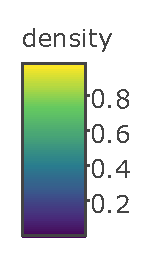
\includegraphics{bookdown_files/figure-latex/us-density-1.pdf}
\caption{\label{fig:us-density}A map of U.S. population density using the
\texttt{state.x77} data from the \textbf{datasets} package.}
\end{figure}

\hypertarget{bars-histograms}{\section{Bars \&
histograms}\label{bars-histograms}}

The \texttt{add\_bars()} and \texttt{add\_histogram()} functions wrap
the \href{https://plot.ly/r/reference/\#bar}{bar} and
\href{https://plot.ly/r/reference/\#histogram}{histogram} plotly.js
trace types. The main difference between them is that bar traces require
bar heights (both \texttt{x} and \texttt{y}), whereas histogram traces
require just a single variable, and plotly.js handles binning in the
browser.\footnote{This has some interesting applications for
  \protect\hyperlink{linked-highlighting}{linked highlighting} as it
  allows for summary statistics to be computed on-the-fly based on a
  selection} And perhaps confusingly, both of these functions can be
used to visualize the distribution of either a numeric or a discrete
variable. So, essentially, the only difference between them is where the
binning occurs.

Figure \ref{fig:numeric} compares the default binning algorithm in
plotly.js to a few different algorithms available in R via the
\texttt{hist()} function. Although plotly.js has the ability to
customize histogram bins via
\href{https://plot.ly/r/reference/\#histogram-xbins}{xbins}/\href{https://plot.ly/r/reference/\#histogram-ybins}{ybins},
R has diverse facilities for estimating the optimal number of bins in a
histogram that we can easily leverage.\footnote{Optimal in this context
  is the number of bins which minimizes the distance between the
  empirical histogram and the underlying density.} The \texttt{hist()}
function alone allows us to reference 3 famous algorithms by name
\citep{Sturges}; \citep{FD}; \citep{hist-scott}, but there are also
packages (e.g.~the \textbf{histogram} package) which extend this
interface to incorporate more methodology \citep{histogram}. The
\texttt{price\_hist()} function below wraps the \texttt{hist()} function
to obtain the binning results, and map those bins to a plotly version of
the histogram using \texttt{add\_bars()}.

\begin{Shaded}
\begin{Highlighting}[]
\NormalTok{p1 <-}\StringTok{ }\KeywordTok{plot_ly}\NormalTok{(diamonds, }\DataTypeTok{x =} \NormalTok{~price) %>%}\StringTok{ }\KeywordTok{add_histogram}\NormalTok{(}\DataTypeTok{name =} \StringTok{"plotly.js"}\NormalTok{)}

\NormalTok{price_hist <-}\StringTok{ }\NormalTok{function(}\DataTypeTok{method =} \StringTok{"FD"}\NormalTok{) \{}
  \NormalTok{h <-}\StringTok{ }\KeywordTok{hist}\NormalTok{(diamonds$price, }\DataTypeTok{breaks =} \NormalTok{method, }\DataTypeTok{plot =} \OtherTok{FALSE}\NormalTok{)}
  \KeywordTok{plot_ly}\NormalTok{(}\DataTypeTok{x =} \NormalTok{h$mids, }\DataTypeTok{y =} \NormalTok{h$counts) %>%}\StringTok{ }\KeywordTok{add_bars}\NormalTok{(}\DataTypeTok{name =} \NormalTok{method)}
\NormalTok{\}}

\KeywordTok{subplot}\NormalTok{(}
  \NormalTok{p1, }\KeywordTok{price_hist}\NormalTok{(), }\KeywordTok{price_hist}\NormalTok{(}\StringTok{"Sturges"}\NormalTok{),  }\KeywordTok{price_hist}\NormalTok{(}\StringTok{"Scott"}\NormalTok{),}
  \DataTypeTok{nrows =} \DecValTok{4}\NormalTok{, }\DataTypeTok{shareX =} \OtherTok{TRUE}
\NormalTok{)}
\end{Highlighting}
\end{Shaded}

\begin{figure}[htbp]
\centering
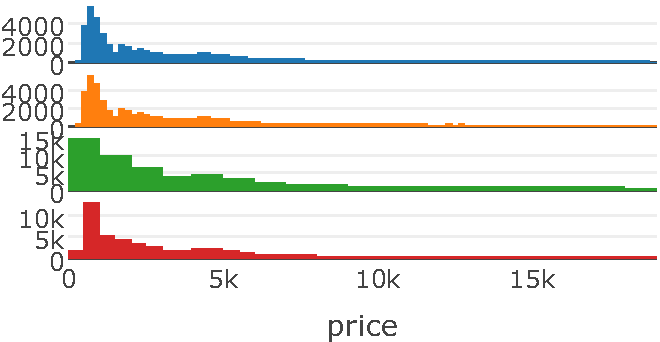
\includegraphics{bookdown_files/figure-latex/numeric-1.pdf}
\caption{\label{fig:numeric}plotly.js's default binning algorithm versus R's
\texttt{hist()} default}
\end{figure}

Figure \ref{fig:discrete} demonstrates two ways of creating a basic bar
chart. Although the visual results are the same, its worth noting the
difference in implementation. The \texttt{add\_histogram()} function
sends all of the observed values to the browser and lets plotly.js
perform the binning. It takes more human effort to perform the binning
in R, but doing so has the benefit of sending less data, and requiring
less computation work of the web browser. In this case, we have only
about 50,000 records, so there is much of a difference in page load
times or page size. However, with 1 Million records, page load time more
than doubles and page size nearly doubles.\footnote{These tests were run
  on Google Chrome and loaded a page with a single bar chart.
  \href{https://www.webpagetest.org/result/160924_DP_JBX/}{Here} are the
  results for \texttt{add\_histogram()} and
  \href{https://www.webpagetest.org/result/160924_QG_JA1/}{here} are the
  results for \texttt{add\_bars()}}

\begin{Shaded}
\begin{Highlighting}[]
\NormalTok{p1 <-}\StringTok{ }\KeywordTok{plot_ly}\NormalTok{(diamonds, }\DataTypeTok{x =} \NormalTok{~cut) %>%}\StringTok{ }\KeywordTok{add_histogram}\NormalTok{()}

\NormalTok{p2 <-}\StringTok{ }\NormalTok{diamonds %>%}
\StringTok{  }\NormalTok{dplyr::}\KeywordTok{count}\NormalTok{(cut) %>%}
\StringTok{  }\KeywordTok{plot_ly}\NormalTok{(}\DataTypeTok{x =} \NormalTok{~cut, }\DataTypeTok{y =} \NormalTok{~n) %>%}\StringTok{ }
\StringTok{  }\KeywordTok{add_bars}\NormalTok{()}

\KeywordTok{subplot}\NormalTok{(p1, p2) %>%}\StringTok{ }\KeywordTok{hide_legend}\NormalTok{()}
\end{Highlighting}
\end{Shaded}

\begin{figure}[htbp]
\centering
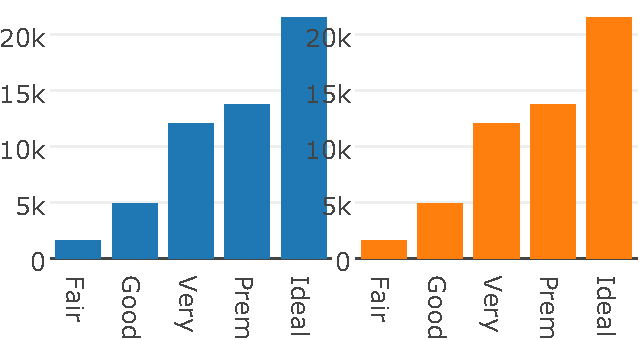
\includegraphics{bookdown_files/figure-latex/discrete-1.pdf}
\caption{\label{fig:discrete}Number of diamonds by cut.}
\end{figure}

\subsection{Multiple numeric
distributions}\label{multiple-numeric-distributions}

It is often useful to see how the numeric distribution changes with
respect to a discrete variable. When using bars to visualize multiple
numeric distributions, I recommend plotting each distribution on its own
axis, rather than trying to overlay them on a single axis.\footnote{It's
  much easier to visualize multiple numeric distributions on a single
  axis using \protect\hyperlink{lines}{lines}}. This is where the
\protect\hyperlink{subplot}{\texttt{subplot()} infrastructure}, and its
support for trellis displays, comes in handy. Figure
\ref{fig:many-prices} shows a trellis display of diamond price by
diamond color. Note how the \texttt{one\_plot()} function defines what
to display on each panel, then a split-apply-recombine strategy is
employed to generate the trellis display.

\begin{Shaded}
\begin{Highlighting}[]
\NormalTok{one_plot <-}\StringTok{ }\NormalTok{function(d) \{}
  \KeywordTok{plot_ly}\NormalTok{(d, }\DataTypeTok{x =} \NormalTok{~price) %>%}
\StringTok{    }\KeywordTok{add_annotations}\NormalTok{(}
      \NormalTok{~}\KeywordTok{paste}\NormalTok{(}\StringTok{"Clarity:"}\NormalTok{, }\KeywordTok{unique}\NormalTok{(clarity)), }\DataTypeTok{x =} \FloatTok{0.5}\NormalTok{, }\DataTypeTok{y =} \DecValTok{1}\NormalTok{, }
      \DataTypeTok{xref =} \StringTok{"paper"}\NormalTok{, }\DataTypeTok{yref =} \StringTok{"paper"}\NormalTok{, }\DataTypeTok{showarrow =} \OtherTok{FALSE}
    \NormalTok{)}
\NormalTok{\}}

\NormalTok{diamonds %>%}
\StringTok{  }\KeywordTok{split}\NormalTok{(.$clarity) %>%}
\StringTok{  }\KeywordTok{lapply}\NormalTok{(one_plot) %>%}\StringTok{ }
\StringTok{  }\KeywordTok{subplot}\NormalTok{(}\DataTypeTok{nrows =} \DecValTok{2}\NormalTok{, }\DataTypeTok{shareX =} \OtherTok{TRUE}\NormalTok{, }\DataTypeTok{titleX =} \OtherTok{FALSE}\NormalTok{) %>%}
\StringTok{  }\KeywordTok{hide_legend}\NormalTok{()}
\end{Highlighting}
\end{Shaded}

\begin{figure}[htbp]
\centering
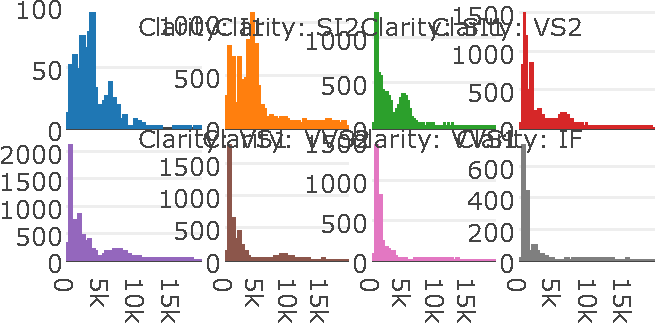
\includegraphics{bookdown_files/figure-latex/many-prices-1.pdf}
\caption{\label{fig:many-prices}A trellis display of diamond price by
diamond color.}
\end{figure}

\subsection{Multiple discrete
distributions}\label{multiple-discrete-distributions}

Visualizing multiple discrete distributions is difficult. The subtle
complexity is due to the fact that both counts and proportions are
important for understanding multi-variate discrete distributions. Figure
\ref{fig:cut-by-clarity} presents diamond counts, divided by both their
cut and clarity, using a grouped bar chart.

\begin{Shaded}
\begin{Highlighting}[]
\KeywordTok{plot_ly}\NormalTok{(diamonds, }\DataTypeTok{x =} \NormalTok{~cut, }\DataTypeTok{color =} \NormalTok{~clarity) %>%}
\StringTok{  }\KeywordTok{add_histogram}\NormalTok{()}
\end{Highlighting}
\end{Shaded}

\begin{figure}[htbp]
\centering
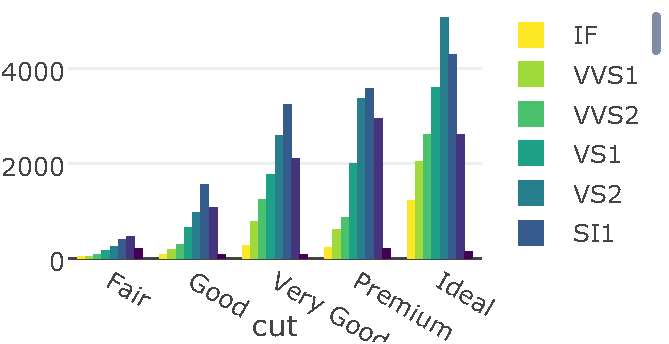
\includegraphics{bookdown_files/figure-latex/cut-by-clarity-1.pdf}
\caption{\label{fig:cut-by-clarity}A grouped bar chart}
\end{figure}

Figure \ref{fig:cut-by-clarity} is useful for comparing the number of
diamonds by clarity, given a type of cut. For instance, within ``Ideal''
diamonds, a cut of ``VS1'' is most popular, ``VS2'' is second most
popular, and ``I1'' the least popular. The distribution of clarity
within ``Ideal'' diamonds seems to be fairly similar to other diamonds,
but it's hard to make this comparison using raw counts. Figure
\ref{fig:cut-by-clarity-prop} makes this comparison easier by showing
the relative frequency of diamonds by clarity, given a cut.

\begin{Shaded}
\begin{Highlighting}[]
\CommentTok{# number of diamonds by cut and clarity (n)}
\NormalTok{cc <-}\StringTok{ }\KeywordTok{count}\NormalTok{(diamonds, cut, clarity)}
\CommentTok{# number of diamonds by cut (nn)}
\NormalTok{cc2 <-}\StringTok{ }\KeywordTok{left_join}\NormalTok{(cc, }\KeywordTok{count}\NormalTok{(cc, cut, }\DataTypeTok{wt =} \NormalTok{n))}
\NormalTok{cc2 %>%}
\StringTok{  }\KeywordTok{mutate}\NormalTok{(}\DataTypeTok{prop =} \NormalTok{n /}\StringTok{ }\NormalTok{nn) %>%}
\StringTok{  }\KeywordTok{plot_ly}\NormalTok{(}\DataTypeTok{x =} \NormalTok{~cut, }\DataTypeTok{y =} \NormalTok{~prop, }\DataTypeTok{color =} \NormalTok{~clarity) %>%}
\StringTok{  }\KeywordTok{add_bars}\NormalTok{() %>%}
\StringTok{  }\KeywordTok{layout}\NormalTok{(}\DataTypeTok{barmode =} \StringTok{"stack"}\NormalTok{)}
\end{Highlighting}
\end{Shaded}

\begin{figure}[htbp]
\centering
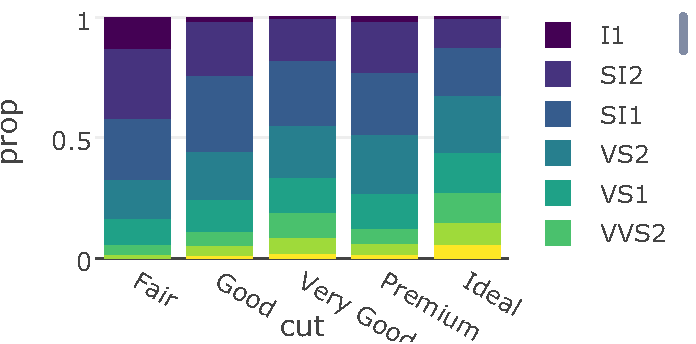
\includegraphics{bookdown_files/figure-latex/cut-by-clarity-prop-1.pdf}
\caption{\label{fig:cut-by-clarity-prop}A stacked bar chart showing the
proportion of clarity within}
\end{figure}

This type of plot, also known as a spine plot, is a special case of a
mosaic plot. In a mosaic plot, you can scale both bar widths and heights
according to discrete distributions. For mosaic plots, I recommend using
the \textbf{ggmosaic} package \citep{ggmosaic}, which implements a
custom \textbf{ggplot2} geom designed for mosaic plots, which we can
convert to plotly via \texttt{ggplotly()}. Figure \ref{fig:ggmosaic}
show a mosaic plot of cut by clarity. Notice how the bar widths are
scaled proportional to the cut frequency.

\begin{Shaded}
\begin{Highlighting}[]
\KeywordTok{library}\NormalTok{(ggmosaic)}
\NormalTok{p <-}\StringTok{ }\KeywordTok{ggplot}\NormalTok{(}\DataTypeTok{data =} \NormalTok{cc) +}
\StringTok{  }\KeywordTok{geom_mosaic}\NormalTok{(}\KeywordTok{aes}\NormalTok{(}\DataTypeTok{weight =} \NormalTok{n, }\DataTypeTok{x =} \KeywordTok{product}\NormalTok{(cut), }\DataTypeTok{fill =} \NormalTok{clarity))}
\CommentTok{#> Error in as.vector(y): attempt to apply non-function}
\KeywordTok{ggplotly}\NormalTok{(p)}
\end{Highlighting}
\end{Shaded}

\begin{figure}[htbp]
\centering
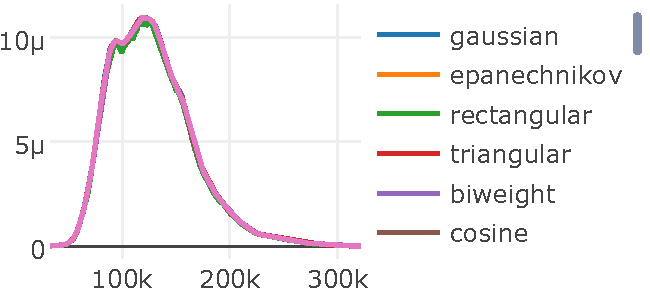
\includegraphics{bookdown_files/figure-latex/ggmosaic-1.pdf}
\caption{\label{fig:ggmosaic}Using ggmosaic and ggplotly() to create
advanced interactive visualizations of categorical data}
\end{figure}

\section{Boxplots}\label{boxplots}

Boxplots encode the five number summary of a numeric variable, and are
more efficient than \href{multiple-numeric-distributions}{trellis
displays of histograms} for comparing many numeric distributions. The
\texttt{add\_boxplot()} function requires one numeric variable, and
guarantees boxplots are
\href{https://plot.ly/r/reference/\#box-orientation}{oriented}
correctly, regardless of whether the numeric variable is placed on the x
or y scale. As Figure \ref{fig:cut-boxes} shows, on the axis orthogonal
to the numeric axis, you can provide a discrete variable (for
conditioning) or supply a single value (to name the axis category).

\begin{Shaded}
\begin{Highlighting}[]
\NormalTok{p <-}\StringTok{ }\KeywordTok{plot_ly}\NormalTok{(diamonds, }\DataTypeTok{y =} \NormalTok{~price, }\DataTypeTok{color =} \KeywordTok{I}\NormalTok{(}\StringTok{"black"}\NormalTok{), }
             \DataTypeTok{alpha =} \FloatTok{0.1}\NormalTok{, }\DataTypeTok{boxpoints =} \StringTok{"suspectedoutliers"}\NormalTok{)}
\NormalTok{p1 <-}\StringTok{ }\NormalTok{p %>%}\StringTok{ }\KeywordTok{add_boxplot}\NormalTok{(}\DataTypeTok{x =} \StringTok{"Overall"}\NormalTok{)}
\NormalTok{p2 <-}\StringTok{ }\NormalTok{p %>%}\StringTok{ }\KeywordTok{add_boxplot}\NormalTok{(}\DataTypeTok{x =} \NormalTok{~cut)}
\KeywordTok{subplot}\NormalTok{(}
  \NormalTok{p1, p2, }\DataTypeTok{shareY =} \OtherTok{TRUE}\NormalTok{,}
  \DataTypeTok{widths =} \KeywordTok{c}\NormalTok{(}\FloatTok{0.2}\NormalTok{, }\FloatTok{0.8}\NormalTok{), }\DataTypeTok{margin =} \DecValTok{0}
\NormalTok{) %>%}\StringTok{ }\KeywordTok{hide_legend}\NormalTok{()}
\end{Highlighting}
\end{Shaded}

\begin{figure}[htbp]
\centering
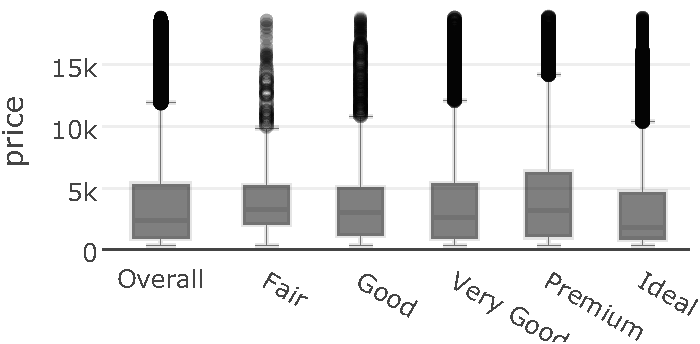
\includegraphics{bookdown_files/figure-latex/cut-boxes-1.pdf}
\caption{\label{fig:cut-boxes}Overall diamond price and price by cut.}
\end{figure}

If you want to partition by more than one discrete variable, I recommend
mapping the interaction of those variables to the discrete axis, and
coloring by the nested variable, as Figure
\ref{fig:cut-by-clarity-boxes} does with diamond clarity and cut.

\begin{Shaded}
\begin{Highlighting}[]
\KeywordTok{plot_ly}\NormalTok{(diamonds, }\DataTypeTok{x =} \NormalTok{~price, }\DataTypeTok{y =} \NormalTok{~}\KeywordTok{interaction}\NormalTok{(clarity, cut)) %>%}
\StringTok{  }\KeywordTok{add_boxplot}\NormalTok{(}\DataTypeTok{color =} \NormalTok{~clarity) %>%}
\StringTok{  }\KeywordTok{layout}\NormalTok{(}\DataTypeTok{yaxis =} \KeywordTok{list}\NormalTok{(}\DataTypeTok{title =} \StringTok{""}\NormalTok{), }\DataTypeTok{margin =} \KeywordTok{list}\NormalTok{(}\DataTypeTok{l =} \DecValTok{100}\NormalTok{))}
\end{Highlighting}
\end{Shaded}

\begin{figure}[htbp]
\centering
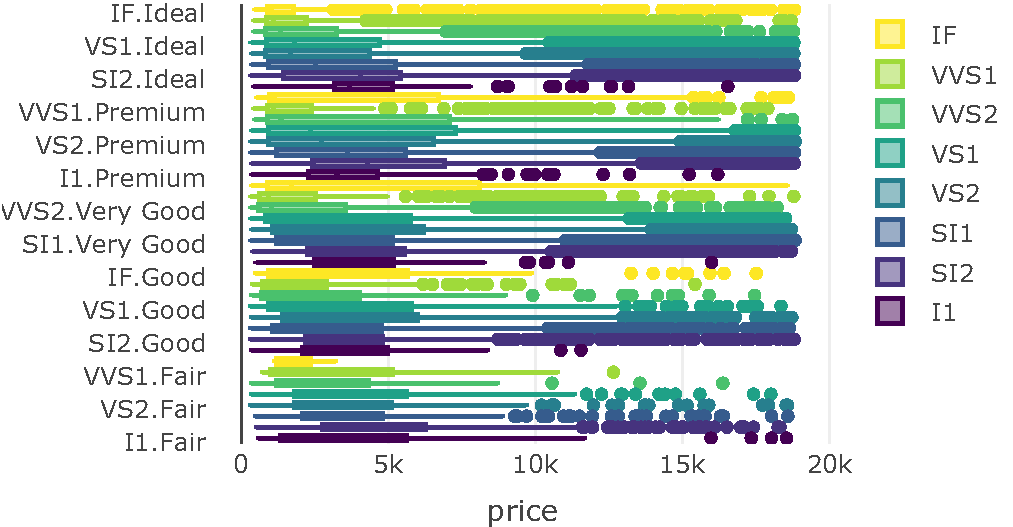
\includegraphics{bookdown_files/figure-latex/cut-by-clarity-boxes-1.pdf}
\caption{\label{fig:cut-by-clarity-boxes}Diamond prices by cut and clarity.}
\end{figure}

It is also helpful to sort the boxplots according to something
meaningful, such as the median price. Figure
\ref{fig:cut-by-clarity-boxes-sorted} presents the same information as
Figure \ref{fig:cut-by-clarity-boxes}, but sorts the boxplots by their
median, and makes it immediately clear that diamonds with a cut of
``SI2'' have the highest diamond price, on average.

\begin{Shaded}
\begin{Highlighting}[]
\NormalTok{d <-}\StringTok{ }\NormalTok{diamonds %>%}
\StringTok{  }\KeywordTok{mutate}\NormalTok{(}\DataTypeTok{cc =} \KeywordTok{interaction}\NormalTok{(clarity, cut))}

\CommentTok{# interaction levels sorted by median price}
\NormalTok{lvls <-}\StringTok{ }\NormalTok{d %>%}
\StringTok{  }\KeywordTok{group_by}\NormalTok{(cc) %>%}
\StringTok{  }\KeywordTok{summarise}\NormalTok{(}\DataTypeTok{m =} \KeywordTok{median}\NormalTok{(price)) %>%}
\StringTok{  }\KeywordTok{arrange}\NormalTok{(m) %>%}
\StringTok{  }\NormalTok{.[[}\StringTok{"cc"}\NormalTok{]]}

\KeywordTok{plot_ly}\NormalTok{(d, }\DataTypeTok{x =} \NormalTok{~price, }\DataTypeTok{y =} \NormalTok{~}\KeywordTok{factor}\NormalTok{(cc, lvls)) %>%}
\StringTok{  }\KeywordTok{add_boxplot}\NormalTok{(}\DataTypeTok{color =} \NormalTok{~clarity) %>%}
\StringTok{  }\KeywordTok{layout}\NormalTok{(}\DataTypeTok{yaxis =} \KeywordTok{list}\NormalTok{(}\DataTypeTok{title =} \StringTok{""}\NormalTok{), }\DataTypeTok{margin =} \KeywordTok{list}\NormalTok{(}\DataTypeTok{l =} \DecValTok{100}\NormalTok{))}
\end{Highlighting}
\end{Shaded}

\begin{figure}[htbp]
\centering
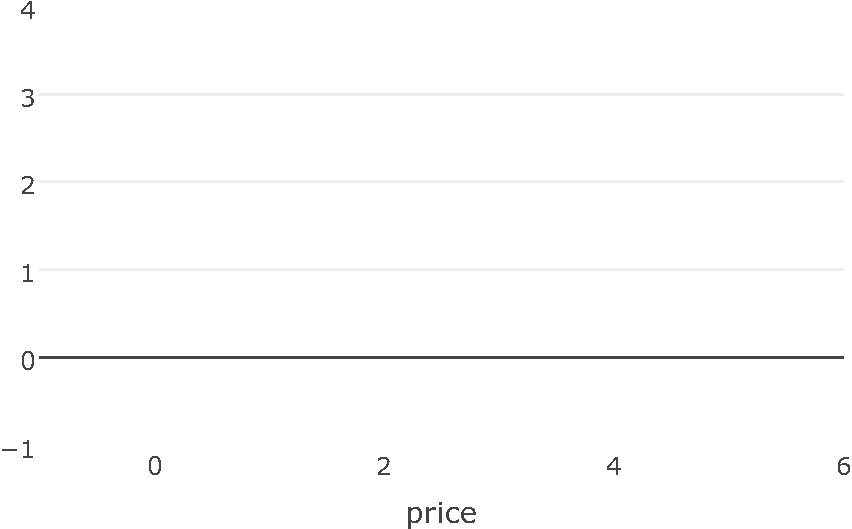
\includegraphics{bookdown_files/figure-latex/cut-by-clarity-boxes-sorted-1.pdf}
\caption{\label{fig:cut-by-clarity-boxes-sorted}Diamond prices by cut and
clarity, sorted by price median.}
\end{figure}

Similar to \texttt{add\_histogram()}, \texttt{add\_boxplot()} sends the
raw data to the browser, and lets plotly.js compute summary statistics.
Unfortunately, plotly.js does not yet allow precomputed statistics for
boxplots.\footnote{Follow the issue here
  \url{https://github.com/plotly/plotly.js/issues/242}}

\section{2D distributions}\label{d-distributions}

\subsection{Rectangular binning in
plotly.js}\label{rectangular-binning-in-plotly.js}

The \textbf{plotly} package provides two functions for displaying
rectangular bins: \texttt{add\_heatmap()} and
\texttt{add\_histogram2d()}. For numeric data, the
\texttt{add\_heatmap()} function is a 2D analog of \texttt{add\_bars()}
(bins must be pre-computed), and the \texttt{add\_histogram2d()}
function is a 2D analog of \texttt{add\_histogram()} (bins can be
computed in the browser). Thus, I recommend \texttt{add\_histogram2d()}
for exploratory purposes, since you don't have to think about how to
perform binning. It also provides a useful
\href{https://plot.ly/r/reference/\#histogram2d-zsmooth}{\texttt{zsmooth}}
attribute for effectively increasing the number of bins (currently,
``best'' performs a
\href{https://en.wikipedia.org/wiki/Bilinear_interpolation}{bi-linear
interpolation}, a type of nearest neighbors algorithm), and
\href{https://plot.ly/r/reference/\#histogram2d-nbinsx}{nbinsx}/\href{https://plot.ly/r/reference/\#histogram2d-nbinsy}{nbinsy}
attributes to set the number of bins in the x and/or y directions.
Figure \ref{fig:histogram2d} compares three different uses of
\texttt{add\_histogram()}: (1) plotly.js' default binning algorithm, (2)
the default plus smoothing, (3) setting the number of bins in the x and
y directions.

\begin{Shaded}
\begin{Highlighting}[]
\NormalTok{p <-}\StringTok{ }\KeywordTok{plot_ly}\NormalTok{(diamonds, }\DataTypeTok{x =} \NormalTok{~}\KeywordTok{log}\NormalTok{(carat), }\DataTypeTok{y =} \NormalTok{~}\KeywordTok{log}\NormalTok{(price))}
\KeywordTok{subplot}\NormalTok{(}
  \KeywordTok{add_histogram2d}\NormalTok{(p) %>%}
\StringTok{    }\KeywordTok{colorbar}\NormalTok{(}\DataTypeTok{title =} \StringTok{"default"}\NormalTok{, }\DataTypeTok{len =} \DecValTok{1}\NormalTok{/}\DecValTok{3}\NormalTok{, }\DataTypeTok{y =} \DecValTok{1}\NormalTok{) %>%}
\StringTok{    }\KeywordTok{layout}\NormalTok{(}\DataTypeTok{xaxis =} \KeywordTok{list}\NormalTok{(}\DataTypeTok{title =} \StringTok{"default"}\NormalTok{)),}
  \KeywordTok{add_histogram2d}\NormalTok{(p, }\DataTypeTok{zsmooth =} \StringTok{"best"}\NormalTok{) %>%}
\StringTok{    }\KeywordTok{colorbar}\NormalTok{(}\DataTypeTok{title =} \StringTok{"zsmooth"}\NormalTok{, }\DataTypeTok{len =} \DecValTok{1}\NormalTok{/}\DecValTok{3}\NormalTok{, }\DataTypeTok{y =} \DecValTok{2}\NormalTok{/}\DecValTok{3} \NormalTok{-}\StringTok{ }\FloatTok{0.05}\NormalTok{) %>%}
\StringTok{    }\KeywordTok{layout}\NormalTok{(}\DataTypeTok{xaxis =} \KeywordTok{list}\NormalTok{(}\DataTypeTok{title =} \StringTok{"zsmooth"}\NormalTok{)),}
  \KeywordTok{add_histogram2d}\NormalTok{(p, }\DataTypeTok{nbinsx =} \DecValTok{60}\NormalTok{, }\DataTypeTok{nbinsy =} \DecValTok{60}\NormalTok{) %>%}
\StringTok{    }\KeywordTok{colorbar}\NormalTok{(}\DataTypeTok{title =} \StringTok{"nbins"}\NormalTok{, }\DataTypeTok{len =} \DecValTok{1}\NormalTok{/}\DecValTok{3}\NormalTok{, }\DataTypeTok{y =} \DecValTok{1}\NormalTok{/}\DecValTok{3} \NormalTok{-}\StringTok{ }\FloatTok{0.1}\NormalTok{) %>%}
\StringTok{    }\KeywordTok{layout}\NormalTok{(}\DataTypeTok{xaxis =} \KeywordTok{list}\NormalTok{(}\DataTypeTok{title =} \StringTok{"nbins"}\NormalTok{)),}
  \DataTypeTok{shareY =} \OtherTok{TRUE}\NormalTok{, }\DataTypeTok{titleX =} \OtherTok{TRUE}
\NormalTok{)}
\end{Highlighting}
\end{Shaded}

\begin{figure}[htbp]
\centering
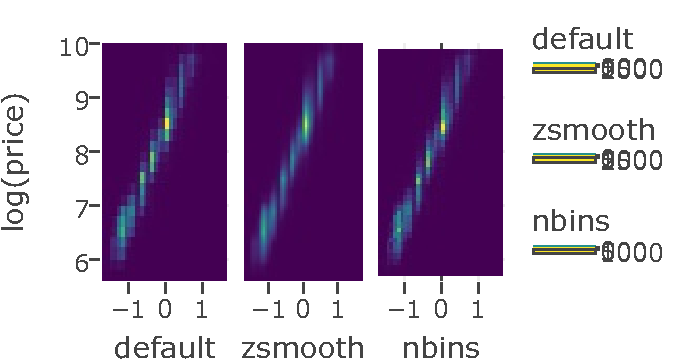
\includegraphics{bookdown_files/figure-latex/histogram2d-1.pdf}
\caption{\label{fig:histogram2d}Three different uses of
\texttt{histogram2d()}}
\end{figure}

\subsection{Rectangular binning in R}\label{rectangular-binning-in-r}

In \protect\hyperlink{bars-histograms}{Bars \& histograms}, we leveraged
a number of algorithms in R for computing the ``optimal'' number of bins
for a histogram, via \texttt{hist()}, and routing those results to
\texttt{add\_bars()}. There is a surprising lack of research and
computational tools for the 2D analog, and among the research that does
exist, solutions usually depend on characteristics of the unknown
underlying distribution, so the typical approach is to assume a Gaussian
form \citep{mde}. Kernel density estimation is another non

Practically speaking, that assumption is not very useful, but thankfully
, and specifically the \texttt{kde2d()} function from the \textbf{MASS}
package, provides a well-supported rule-of-thumb.

\begin{Shaded}
\begin{Highlighting}[]
\NormalTok{kde_count <-}\StringTok{ }\NormalTok{function(x, y, ...) \{}
  \NormalTok{kde <-}\StringTok{ }\NormalTok{MASS::}\KeywordTok{kde2d}\NormalTok{(x, y, ...)}
  \NormalTok{df <-}\StringTok{ }\KeywordTok{with}\NormalTok{(kde, }\KeywordTok{setNames}\NormalTok{(}\KeywordTok{expand.grid}\NormalTok{(x, y), }\KeywordTok{c}\NormalTok{(}\StringTok{"x"}\NormalTok{, }\StringTok{"y"}\NormalTok{)))}
  \NormalTok{df$count <-}\StringTok{ }\KeywordTok{with}\NormalTok{(kde, }\KeywordTok{c}\NormalTok{(z) *}\StringTok{ }\KeywordTok{length}\NormalTok{(x) *}\StringTok{ }\KeywordTok{diff}\NormalTok{(x)[}\DecValTok{1}\NormalTok{] *}\StringTok{ }\KeywordTok{diff}\NormalTok{(y)[}\DecValTok{1}\NormalTok{])}
  \KeywordTok{data.frame}\NormalTok{(df)}
\NormalTok{\}}

\NormalTok{kd <-}\StringTok{ }\KeywordTok{with}\NormalTok{(diamonds, }\KeywordTok{kde_count}\NormalTok{(}\KeywordTok{log}\NormalTok{(carat), }\KeywordTok{log}\NormalTok{(price), }\DataTypeTok{n =} \DecValTok{30}\NormalTok{))}
\KeywordTok{plot_ly}\NormalTok{(kd, }\DataTypeTok{x =} \NormalTok{~x, }\DataTypeTok{y =} \NormalTok{~y, }\DataTypeTok{z =} \NormalTok{~count) %>%}\StringTok{ }
\StringTok{  }\KeywordTok{add_heatmap}\NormalTok{() %>%}
\StringTok{  }\KeywordTok{colorbar}\NormalTok{(}\DataTypeTok{title =} \StringTok{"Number of diamonds"}\NormalTok{)}
\end{Highlighting}
\end{Shaded}

\begin{figure}[htbp]
\centering
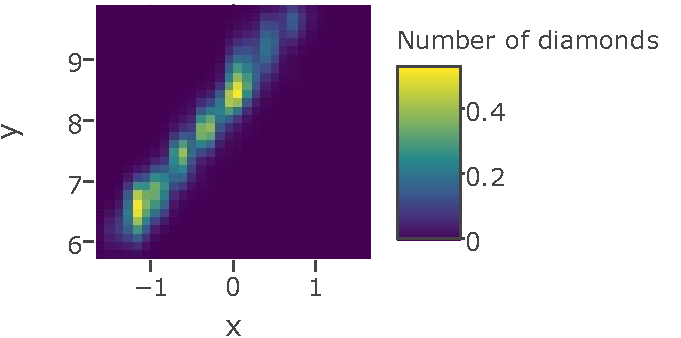
\includegraphics{bookdown_files/figure-latex/heatmap-corr-diamonds-1.pdf}
\caption{\label{fig:heatmap-corr-diamonds}2D Density estimation via the
\texttt{kde2d()} function}
\end{figure}

\subsection{Basic heatmaps}\label{basic-heatmaps}

The \texttt{add\_heatmap()} function can also handle categorical x and y
variables.

\begin{Shaded}
\begin{Highlighting}[]
\NormalTok{corr <-}\StringTok{ }\KeywordTok{cor}\NormalTok{(diamonds[}\KeywordTok{vapply}\NormalTok{(diamonds, is.numeric, }\KeywordTok{logical}\NormalTok{(}\DecValTok{1}\NormalTok{))])}
\KeywordTok{plot_ly}\NormalTok{(}\DataTypeTok{x =} \KeywordTok{rownames}\NormalTok{(corr), }\DataTypeTok{y =} \KeywordTok{colnames}\NormalTok{(corr), }\DataTypeTok{z =} \NormalTok{corr) %>%}
\StringTok{  }\KeywordTok{add_heatmap}\NormalTok{() %>%}
\StringTok{  }\KeywordTok{colorbar}\NormalTok{(}\DataTypeTok{limits =} \KeywordTok{c}\NormalTok{(-}\DecValTok{1}\NormalTok{, }\DecValTok{1}\NormalTok{))}
\end{Highlighting}
\end{Shaded}

\begin{figure}[htbp]
\centering
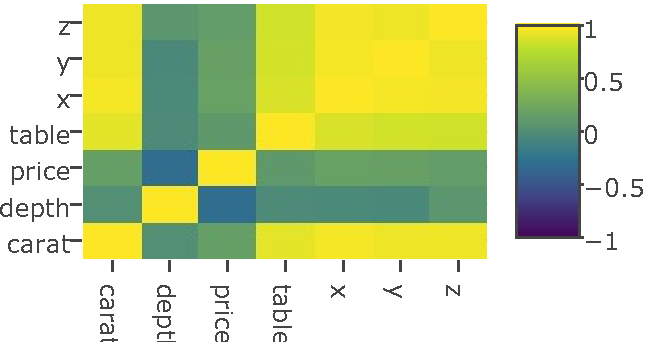
\includegraphics{bookdown_files/figure-latex/unnamed-chunk-26-1.pdf}
\caption{}
\end{figure}

A heatmap with categorical axes is basically a two-way table. The
\texttt{Titanic} dataset is a four-way table that we can put into a tidy
data frame using the \texttt{tidy()} function from the \textbf{broom}
package.

\begin{Shaded}
\begin{Highlighting}[]
\NormalTok{broom::}\KeywordTok{tidy}\NormalTok{(Titanic) %>%}
\StringTok{  }\KeywordTok{plot_ly}\NormalTok{(}\DataTypeTok{x =} \NormalTok{~}\KeywordTok{interaction}\NormalTok{(Age, Survived), }\DataTypeTok{y =} \NormalTok{~}\KeywordTok{interaction}\NormalTok{(Class, Sex)) %>%}
\StringTok{  }\KeywordTok{add_heatmap}\NormalTok{(}\DataTypeTok{z =} \NormalTok{~Freq)}
\end{Highlighting}
\end{Shaded}

\begin{figure}[htbp]
\centering
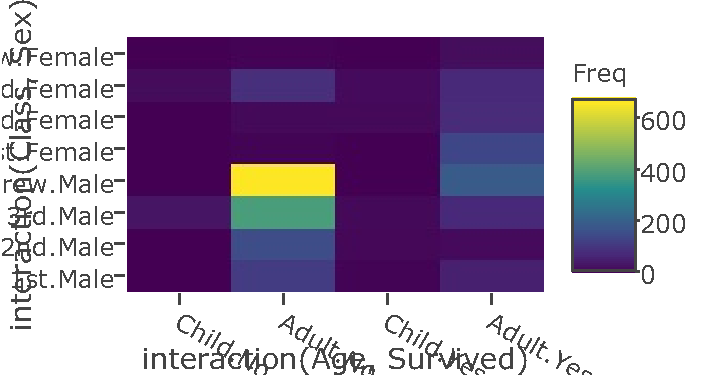
\includegraphics{bookdown_files/figure-latex/unnamed-chunk-27-1.pdf}
\caption{}
\end{figure}

\begin{Shaded}
\begin{Highlighting}[]


\CommentTok{#one_heatmap <- function(d) \{}
\CommentTok{#  plot_ly(d, x = ~Class, y = ~Sex) %>% }
\CommentTok{#    add_heatmap(z = ~Freq) %>%}
\CommentTok{#    add_annotations(}
\CommentTok{#      ~unique(paste(Age, Survived, sep = ", ")), x = 0.5, y = 1, }
\CommentTok{#      yanchor = "bottom", xanchor = "middle",}
\CommentTok{#      xref = "paper", yref = "paper", showarrow = FALSE}
\CommentTok{#    )}
\CommentTok{#\}}
\CommentTok{#}
\CommentTok{#tidy(Titanic) %>%}
\CommentTok{#  group_by(Age, Survived) %>%}
\CommentTok{#  do(p = one_heatmap(.)) %>%}
\CommentTok{#  subplot(}
\CommentTok{#    nrows = 2, margin = c(0.01, 0.01, 0.04, 0.04),}
\CommentTok{#    shareX = TRUE, shareY = TRUE, }
\CommentTok{#    titleY = FALSE, titleX = FALSE}
\CommentTok{#  )}
\end{Highlighting}
\end{Shaded}

\subsection{Contours}\label{contours}

\begin{Shaded}
\begin{Highlighting}[]
\KeywordTok{plot_ly}\NormalTok{(diamonds, }\DataTypeTok{x =} \NormalTok{~cut, }\DataTypeTok{y =} \NormalTok{~clarity) %>%}\StringTok{ }
\StringTok{  }\KeywordTok{add_histogram2dcontour}\NormalTok{()}
\end{Highlighting}
\end{Shaded}

\begin{figure}[htbp]
\centering
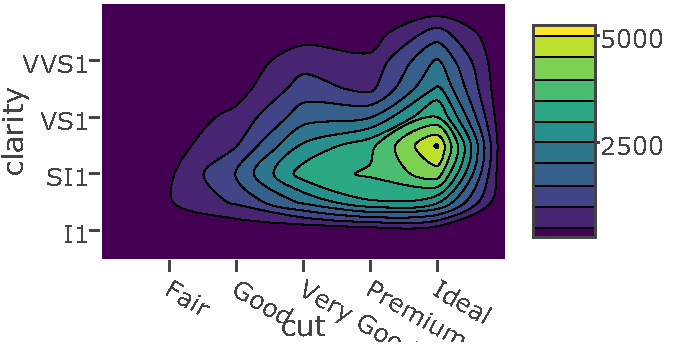
\includegraphics{bookdown_files/figure-latex/unnamed-chunk-28-1.pdf}
\caption{}
\end{figure}

\section{3D plots}\label{d-plots}

\subsection{Surface}\label{surface}

\subsection{Mesh}\label{mesh}

\section{Annotations}\label{annotations}

The \texttt{add\_annotations()} function

\hypertarget{subplot}{\chapter{Arranging multiple views}\label{subplot}}

The \texttt{subplot()} function provides a flexible interface for
arranging multiple \textbf{plotly} plots in a single view. It is more
flexible than most trellis display frameworks (e.g., ggplot2's
\texttt{facet\_wrap()}) as you don't have to condition on a value of
common variable in each display \citep{trellis}. Its capabilities and
interface is similar to the \texttt{grid.arrange()} function from the
\textbf{gridExtra} package, which allows you to arrange multiple
\textbf{grid} grobs in a single view, effectively providing a way to
arrange (possibly unrelated) \textbf{ggplot2} and/or \textbf{lattice}
plots in a single view \citep{base}; \citep{gridExtra}; \citep{lattice}.
The simplest way to use it is to pass plotly objects directly to
\texttt{subplot()}.

\begin{Shaded}
\begin{Highlighting}[]
\KeywordTok{library}\NormalTok{(plotly)}
\NormalTok{p1 <-}\StringTok{ }\KeywordTok{plot_ly}\NormalTok{(economics, }\DataTypeTok{x =} \NormalTok{~date, }\DataTypeTok{y =} \NormalTok{~unemploy, }\DataTypeTok{name =} \StringTok{"unemploy"}\NormalTok{) %>%}\StringTok{ }\KeywordTok{add_lines}\NormalTok{()}
\NormalTok{p2 <-}\StringTok{ }\KeywordTok{plot_ly}\NormalTok{(economics, }\DataTypeTok{x =} \NormalTok{~date, }\DataTypeTok{y =} \NormalTok{~uempmed, }\DataTypeTok{name =} \StringTok{"uempmed"}\NormalTok{) %>%}\StringTok{ }\KeywordTok{add_lines}\NormalTok{()}
\KeywordTok{subplot}\NormalTok{(p1, p2)}
\end{Highlighting}
\end{Shaded}

\begin{figure}[htbp]
\centering
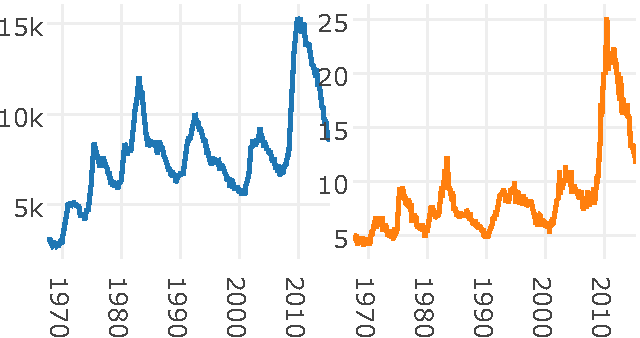
\includegraphics{bookdown_files/figure-latex/unnamed-chunk-29-1.pdf}
\caption{}
\end{figure}

Although \texttt{subplot()} accepts an arbitrary number of plot objects,
passing a \emph{list} of plots can save typing and redundant code when
dealing with a large number of plots. To demonstrate, let's create one
time series for each variable in the \texttt{economics} dataset and
share the x-axis so that zoom/pan events are synchronized across each
series:

\begin{Shaded}
\begin{Highlighting}[]
\NormalTok{vars <-}\StringTok{ }\KeywordTok{setdiff}\NormalTok{(}\KeywordTok{names}\NormalTok{(economics), }\StringTok{"date"}\NormalTok{)}
\NormalTok{plots <-}\StringTok{ }\KeywordTok{lapply}\NormalTok{(vars, function(var) \{}
  \KeywordTok{plot_ly}\NormalTok{(economics, }\DataTypeTok{x =} \NormalTok{~date, }\DataTypeTok{y =} \KeywordTok{as.formula}\NormalTok{(}\KeywordTok{paste0}\NormalTok{(}\StringTok{"~"}\NormalTok{, var)), }\DataTypeTok{name =} \NormalTok{var) %>%}
\StringTok{    }\KeywordTok{add_lines}\NormalTok{()}
\NormalTok{\})}
\KeywordTok{subplot}\NormalTok{(plots, }\DataTypeTok{nrows =} \KeywordTok{length}\NormalTok{(plots), }\DataTypeTok{shareX =} \OtherTok{TRUE}\NormalTok{, }\DataTypeTok{titleX =} \OtherTok{FALSE}\NormalTok{)}
\end{Highlighting}
\end{Shaded}

\begin{figure}[htbp]
\centering
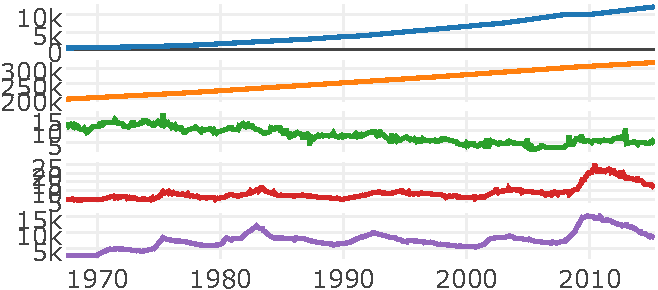
\includegraphics{bookdown_files/figure-latex/economics-1.pdf}
\caption{\label{fig:economics}Five different economic variables on different
y scales and a common x scale. Zoom and pan events in the x-direction
are synchronized across plots.}
\end{figure}

A plotly subplot is a single plotly graph with multiple traces anchored
on different axes. If you pre-specify an
\href{https://plot.ly/r/reference/\#scatter-yaxis}{axis ID} for each
trace, \texttt{subplot()} will respect that ID. Figure
\ref{fig:prepopulate} uses this fact in correspondence with the fact
that mapping a discrete variable to \texttt{color} creates one trace per
value. In addition to providing more control over trace placement, this
provides a convenient way to control coloring (we could have
\texttt{symbol}/\texttt{linetype} to acheive the same effect).

\begin{Shaded}
\begin{Highlighting}[]
\NormalTok{economics %>%}
\StringTok{  }\NormalTok{tidyr::}\KeywordTok{gather}\NormalTok{(variable, value, -date) %>%}
\StringTok{  }\KeywordTok{transform}\NormalTok{(}\DataTypeTok{id =} \KeywordTok{as.integer}\NormalTok{(}\KeywordTok{factor}\NormalTok{(variable))) %>%}
\StringTok{  }\KeywordTok{plot_ly}\NormalTok{(}\DataTypeTok{x =} \NormalTok{~date, }\DataTypeTok{y =} \NormalTok{~value, }\DataTypeTok{color =} \NormalTok{~variable, }\DataTypeTok{colors =} \StringTok{"Dark2"}\NormalTok{,}
          \DataTypeTok{yaxis =} \NormalTok{~}\KeywordTok{paste0}\NormalTok{(}\StringTok{"y"}\NormalTok{, id)) %>%}
\StringTok{  }\KeywordTok{add_lines}\NormalTok{() %>%}
\StringTok{  }\KeywordTok{subplot}\NormalTok{(}\DataTypeTok{nrows =} \DecValTok{5}\NormalTok{, }\DataTypeTok{shareX =} \OtherTok{TRUE}\NormalTok{)}
\end{Highlighting}
\end{Shaded}

\begin{figure}[htbp]
\centering
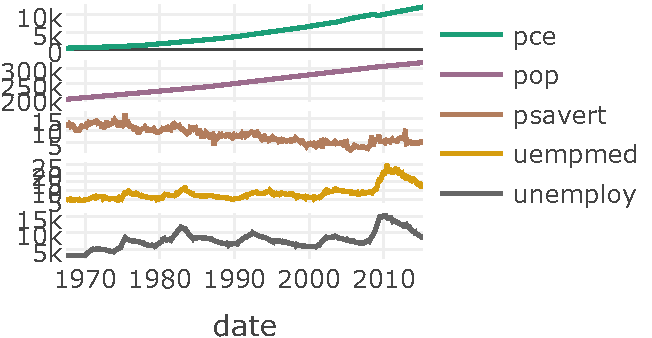
\includegraphics{bookdown_files/figure-latex/prepopulate-1.pdf}
\caption{\label{fig:prepopulate}Pre-populating y axis IDs.}
\end{figure}

Conceptually, \texttt{subplot()} provides a way to place a collection of
plots into a table with a given number of rows and columns. The number
of rows (and, by consequence, the number of columns) is specified via
the \texttt{nrows} argument. By default each row/column shares an equal
proportion of the overall height/width, but as shown in the diagram
below, that default can be changed via the \texttt{heights} and
\texttt{widths} arguments.

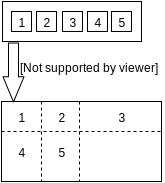
\includegraphics{images/proportions.svg}

This flexibility is quite useful for a number of visualizations, for
example, a joint density plot (the new
\href{https://github.com/talgalili/heatmaply}{heatmaply} package is
another good example).

\begin{Shaded}
\begin{Highlighting}[]
\NormalTok{x <-}\StringTok{ }\KeywordTok{rnorm}\NormalTok{(}\DecValTok{100}\NormalTok{)}
\NormalTok{y <-}\StringTok{ }\KeywordTok{rnorm}\NormalTok{(}\DecValTok{100}\NormalTok{)}
\NormalTok{s <-}\StringTok{ }\KeywordTok{subplot}\NormalTok{(}
  \KeywordTok{plot_ly}\NormalTok{(}\DataTypeTok{x =} \NormalTok{x, }\DataTypeTok{type =} \StringTok{"histogram"}\NormalTok{, }\DataTypeTok{color =} \KeywordTok{I}\NormalTok{(}\StringTok{"black"}\NormalTok{)), }
  \KeywordTok{plotly_empty}\NormalTok{(), }
  \KeywordTok{plot_ly}\NormalTok{(}\DataTypeTok{x =} \NormalTok{x, }\DataTypeTok{y =} \NormalTok{y, }\DataTypeTok{color =} \KeywordTok{I}\NormalTok{(}\StringTok{"black"}\NormalTok{)), }
  \KeywordTok{plot_ly}\NormalTok{(}\DataTypeTok{y =} \NormalTok{y, }\DataTypeTok{color =} \KeywordTok{I}\NormalTok{(}\StringTok{"black"}\NormalTok{)),}
  \DataTypeTok{nrows =} \DecValTok{2}\NormalTok{, }\DataTypeTok{heights =} \KeywordTok{c}\NormalTok{(}\FloatTok{0.2}\NormalTok{, }\FloatTok{0.8}\NormalTok{), }\DataTypeTok{widths =} \KeywordTok{c}\NormalTok{(}\FloatTok{0.8}\NormalTok{, }\FloatTok{0.2}\NormalTok{), }
  \DataTypeTok{shareX =} \OtherTok{TRUE}\NormalTok{, }\DataTypeTok{shareY =} \OtherTok{TRUE}\NormalTok{, }\DataTypeTok{titleX =} \OtherTok{FALSE}\NormalTok{, }\DataTypeTok{titleY =} \OtherTok{FALSE}
\NormalTok{)}
\KeywordTok{layout}\NormalTok{(s, }\DataTypeTok{showlegend =} \OtherTok{FALSE}\NormalTok{)}
\end{Highlighting}
\end{Shaded}

\begin{figure}[htbp]
\centering
\includegraphics{bookdown_files/figure-latex/unnamed-chunk-31-1.pdf}
\caption{}
\end{figure}

Note that, since \texttt{subplot()} returns a plotly object, any
\href{https://plot.ly/r/reference/\#layout}{layout attribute} can be
modified downstream via \texttt{layout()}.

\section{Recursive subplots}\label{recursive-subplots}

The \texttt{subplot()} function is designed to work recursively so that
you can have subplots of subplots. This idea is useful when your desired
layout doesn't conform to the table structure described in the previous
section. In fact, you can think of a subplot of subplots like a
spreadsheet with merged cells.

\includegraphics{images/subplot.svg}

\begin{Shaded}
\begin{Highlighting}[]
\NormalTok{plotList <-}\StringTok{ }\NormalTok{function(nplots) \{}
  \KeywordTok{lapply}\NormalTok{(}\KeywordTok{seq_len}\NormalTok{(nplots), function(x) }\KeywordTok{plot_ly}\NormalTok{())}
\NormalTok{\}}
\NormalTok{s1 <-}\StringTok{ }\KeywordTok{subplot}\NormalTok{(}\KeywordTok{plotList}\NormalTok{(}\DecValTok{6}\NormalTok{), }\DataTypeTok{nrows =} \DecValTok{2}\NormalTok{, }\DataTypeTok{shareX =} \OtherTok{TRUE}\NormalTok{, }\DataTypeTok{shareY =} \OtherTok{TRUE}\NormalTok{)}
\NormalTok{s2 <-}\StringTok{ }\KeywordTok{subplot}\NormalTok{(}\KeywordTok{plotList}\NormalTok{(}\DecValTok{2}\NormalTok{), }\DataTypeTok{shareY =} \OtherTok{TRUE}\NormalTok{)}
\KeywordTok{subplot}\NormalTok{(s1, s2, }\KeywordTok{plot_ly}\NormalTok{(), }\DataTypeTok{nrows =} \DecValTok{3}\NormalTok{, }\DataTypeTok{margin =} \FloatTok{0.04}\NormalTok{, }\DataTypeTok{heights =} \KeywordTok{c}\NormalTok{(}\FloatTok{0.6}\NormalTok{, }\FloatTok{0.3}\NormalTok{, }\FloatTok{0.1}\NormalTok{))}
\end{Highlighting}
\end{Shaded}

\begin{figure}[htbp]
\centering
\includegraphics{bookdown_files/figure-latex/unnamed-chunk-33-1.pdf}
\caption{}
\end{figure}

The concept is particularly useful when you want plot(s) in a given row
to have different widths from plot(s) in another row.

\begin{Shaded}
\begin{Highlighting}[]
\CommentTok{# specify some map projection/options}
\NormalTok{g <-}\StringTok{ }\KeywordTok{list}\NormalTok{(}
  \DataTypeTok{scope =} \StringTok{'usa'}\NormalTok{,}
  \DataTypeTok{projection =} \KeywordTok{list}\NormalTok{(}\DataTypeTok{type =} \StringTok{'albers usa'}\NormalTok{),}
  \DataTypeTok{lakecolor =} \KeywordTok{toRGB}\NormalTok{(}\StringTok{'white'}\NormalTok{)}
\NormalTok{)}
\CommentTok{# create a map of population density}
\NormalTok{density <-}\StringTok{ }\NormalTok{state.x77[, }\StringTok{"Population"}\NormalTok{] /}\StringTok{ }\NormalTok{state.x77[, }\StringTok{"Area"}\NormalTok{]}
\NormalTok{map <-}\StringTok{ }\KeywordTok{plot_geo}\NormalTok{(}\DataTypeTok{z =} \NormalTok{~density, }\DataTypeTok{text =} \NormalTok{state.name, }
                \DataTypeTok{locations =} \NormalTok{state.abb, }\DataTypeTok{locationmode =} \StringTok{'USA-states'}\NormalTok{) %>%}
\StringTok{  }\KeywordTok{layout}\NormalTok{(}\DataTypeTok{geo =} \NormalTok{g)}
\CommentTok{# create a bunch of horizontal bar charts }
\NormalTok{vars <-}\StringTok{ }\KeywordTok{colnames}\NormalTok{(state.x77)}
\NormalTok{barcharts <-}\StringTok{ }\KeywordTok{lapply}\NormalTok{(vars, function(var) \{}
  \KeywordTok{plot_ly}\NormalTok{(}\DataTypeTok{x =} \NormalTok{state.x77[, var], }\DataTypeTok{y =} \NormalTok{state.name) %>%}
\StringTok{    }\KeywordTok{add_bars}\NormalTok{(}\DataTypeTok{orientation =} \StringTok{"h"}\NormalTok{, }\DataTypeTok{name =} \NormalTok{var) %>%}
\StringTok{    }\KeywordTok{layout}\NormalTok{(}\DataTypeTok{showlegend =} \OtherTok{FALSE}\NormalTok{, }\DataTypeTok{hovermode =} \StringTok{"y"}\NormalTok{,}
           \DataTypeTok{yaxis =} \KeywordTok{list}\NormalTok{(}\DataTypeTok{showticklabels =} \OtherTok{FALSE}\NormalTok{))}
\NormalTok{\})}
\KeywordTok{subplot}\NormalTok{(}
  \KeywordTok{subplot}\NormalTok{(barcharts, }\DataTypeTok{margin =} \FloatTok{0.01}\NormalTok{), map, }
  \DataTypeTok{nrows =} \DecValTok{2}\NormalTok{, }\DataTypeTok{heights =} \KeywordTok{c}\NormalTok{(}\FloatTok{0.3}\NormalTok{, }\FloatTok{0.7}\NormalTok{)}
\NormalTok{)}
\end{Highlighting}
\end{Shaded}

\begin{figure}[htbp]
\centering
\includegraphics{bookdown_files/figure-latex/unnamed-chunk-34-1.pdf}
\caption{}
\end{figure}

\section{ggplot2 subplots}\label{ggplot2-subplots}

The \texttt{subplot()} function also understands ggplot2 objects, and
converts them to an interactive web-based version via
\texttt{ggplotly()} before arranging them in the final layout.

\begin{Shaded}
\begin{Highlighting}[]
\NormalTok{e <-}\StringTok{ }\NormalTok{tidyr::}\KeywordTok{gather}\NormalTok{(economics, variable, value, -date)}
\NormalTok{gg1 <-}\StringTok{ }\KeywordTok{ggplot}\NormalTok{(e, }\KeywordTok{aes}\NormalTok{(date, value)) +}\StringTok{ }\KeywordTok{geom_line}\NormalTok{() +}
\StringTok{  }\KeywordTok{facet_wrap}\NormalTok{(~variable, }\DataTypeTok{scales =} \StringTok{"free_y"}\NormalTok{, }\DataTypeTok{ncol =} \DecValTok{1}\NormalTok{)}
\NormalTok{gg2 <-}\StringTok{ }\KeywordTok{ggplot}\NormalTok{(e, }\KeywordTok{aes}\NormalTok{(}\KeywordTok{factor}\NormalTok{(}\DecValTok{1}\NormalTok{), value)) +}\StringTok{ }\KeywordTok{geom_violin}\NormalTok{() +}
\StringTok{  }\KeywordTok{facet_wrap}\NormalTok{(~variable, }\DataTypeTok{scales =} \StringTok{"free_y"}\NormalTok{, }\DataTypeTok{ncol =} \DecValTok{1}\NormalTok{) +}\StringTok{ }
\StringTok{  }\KeywordTok{theme}\NormalTok{(}\DataTypeTok{axis.text =} \KeywordTok{element_blank}\NormalTok{(), }\DataTypeTok{axis.ticks =} \KeywordTok{element_blank}\NormalTok{())}
\KeywordTok{subplot}\NormalTok{(gg1, gg2) %>%}\StringTok{ }\KeywordTok{layout}\NormalTok{(}\DataTypeTok{margin =} \KeywordTok{list}\NormalTok{(}\DataTypeTok{l =} \DecValTok{50}\NormalTok{))}
\end{Highlighting}
\end{Shaded}

\begin{figure}[htbp]
\centering
\includegraphics{bookdown_files/figure-latex/unnamed-chunk-35-1.pdf}
\caption{}
\end{figure}

\chapter{Animating views}\label{animating-views}

\begin{rmdwarning}
The code is this section is still under development and is likely to
change. To run any of the code you see in this section, you'll need this
developmental version of the package:
\texttt{devtools::install\_github("ropensci/plotly\#741")}
\end{rmdwarning}

Both \texttt{plot\_ly()} and \texttt{ggplotly()} understand a
\texttt{frame} aesthetic.

\begin{Shaded}
\begin{Highlighting}[]
\KeywordTok{data}\NormalTok{(gapminder, }\DataTypeTok{package =} \StringTok{"gapminder"}\NormalTok{)}
\NormalTok{p <-}\StringTok{ }\KeywordTok{ggplot}\NormalTok{(gapminder, }\KeywordTok{aes}\NormalTok{(gdpPercap, lifeExp, }\DataTypeTok{size =} \NormalTok{pop, }
                           \DataTypeTok{color =} \NormalTok{continent, }\DataTypeTok{frame =} \NormalTok{year)) +}
\StringTok{  }\KeywordTok{geom_point}\NormalTok{() +}
\StringTok{  }\KeywordTok{scale_x_log10}\NormalTok{()}

\KeywordTok{ggplotly}\NormalTok{(p)}
\end{Highlighting}
\end{Shaded}

IDEAS: * Grand tour * Demonstrate high variance in density estimation
via binning (i.e., same data and different anchor points for the bins
can result in very different values for the binned frequencies)

\chapter{Multiple linked views}\label{multiple-linked-views}

\begin{rmdwarning}
The code is this section is still under development and is likely to
change. To run any of the code you see in this section, you'll need this
developmental version of the package:
\texttt{devtools::install\_github("ropensci/plotly\#554")}
\end{rmdwarning}

Multiple linked views is a concept that has existed in many forms within
the statistical graphics and information visualization community for
many years \citep{brushing-scatterplots}; \citep{ggobi:2007};
\citep{Ahlberg:1997tb}. \citet{Cook:2007uk} provides nice motivation for
and definition of multiple linked views:

\begin{quote}
Multiple linked views are the optimal framework for posing queries about
data. A user should be able to pose a query graphically, and a computer
should be able to present the response graphically as well. Both query
and response should occur in the same visual field. This calls for a
mechanism that links the graphical query to the graphical response. A
graphical user interface that has such linking mechanisms is an
implementation of the notion of ``multiple linked views.''
\end{quote}

There are a number of R packages that provide a graphics rendering
toolkits with built-in support for multiple linked views. Some are
implemented as desktop applications \citep{rggobi}; \citep{cranvas};
\citep{iPlots}; \citep{loon} while others are within a web-based
environment \citep{animint}; \citep{ggvis}; \citep{rbokeh}. In addition
to being easier to share, the advantage of using web-based option(s) is
that we can link views across different systems. To date, the most
versatile tool for linking arbitrary views in R is \textbf{shiny}
\citep{shiny}, which provides a reactive programming framework for
authoring web applications powered by R.
\protect\hyperlink{linking-views-with-shiny}{Linking views with shiny}
explains how to access plotly events on a shiny server, and informing
related views about the events.

Although \textbf{shiny} apps provide a tremendous amount of flexibility
when linking views, deploying and sharing shiny apps is way more
complicated than a standalone HTML file. When you print a plotly object
(or any object built on top of the \textbf{htmlwidgets}
\citep{htmlwidgets} infrastructure) it produces a standalone HTML file
with some interactivity baked into it. The \textbf{plotly} package is
unique in the sense that you can link multiple views without shiny in
three different ways: inside the same plotly object, link multiple
plotly objects, or even link to other htmlwidget packages such as
\textbf{leaflet} \citep{leaflet}. Furthermore, since plotly.js has some
built-in support for performing statistical summaries, in some cases, we
can produce aggregated views of selected data.
\protect\hyperlink{linking-views-with-shiny}{Linking views without
shiny} explains this framework in detail through a series of examples.

Before exploring the two different approaches for linking views, it can
be useful to understand a bit about how interactive graphics systems
work, in general. \citet{viewing-pipeline} and \citet{plumbing} discuss
the fundamental elements that all interactive graphics systems must
possess -- the most important being the concept of a data-plot-pipeline.
As \citet{plumbing} states: ``A pipeline controls the transformation
from data to graphical objects on our screens''. Most, if not all, of
the software discussed in this work describes systems implemented as
desktop applications, where the pipeline resides on a single machine.
While this is convenient for developers, it impedes the user's ability
to share their work with others.

Figure \ref{fig:server-client} provides a simple visual depiction of the
two options available when implementing the pipeline within a web-based
environment. \protect\hyperlink{linking-views-with-shiny}{Linking views
without shiny} explores cases where the pipeline resides entirely within
a client's web-browser, without any calls to a seperate process. This is
highly desirable because visualizations are then easily shared and
viewed from a single file, without any software requirements (besides a
web browser). On the other hand, it is a restrictive environment for
statistical computing since we can not directly leverage R's
computational facilities.\footnote{If the number of possible selection
  states is small, it may be possible to pre-compute all possible
  (statistical) results, and navigate them without recomputing on the
  fly. TODO: provide an example!!} On other words, whenever the pipeline
involves re-computing a statistical model, or performing a complicated
aggregation, I suggest
\protect\hyperlink{linking-views-with-shiny}{linking views with shiny}.

\begin{figure}[htbp]
\centering
\includegraphics{images/server-client.pdf}
\caption{\label{fig:server-client}A visual depiction of the different
approaches to implementing a pipeline in a web-based environment. The R
package \textbf{shiny} exposes the pipeline to users in R, which
requires a web server for viewing. The R package \textbf{crosstalk} will
allow developers to implement and expose the pipeline on both the server
and client levels.}
\end{figure}

\hypertarget{linking-views-with-shiny}{\section{Linking views with
shiny}\label{linking-views-with-shiny}}

\subsection{Accessing events in shiny}\label{accessing-events-in-shiny}

The plotly.js library emits custom events when a user interacts directly
with a graph. The \texttt{event\_data()} function provides a mechanism
for accessing the data corresponding to those events within a shiny app.
The shiny app in Figure \ref{fig:plotlyEvents} is designed to
demonstrate the most useful plotly events one may access via
\texttt{event\_data()}: mouse hover (\texttt{"plotly\_hover"}), click
(\texttt{"plotly\_click"}), and click+drag
(\texttt{"plotly\_selected"}). All of these events return selections on
the data scale, not on a pixel scale, which is useful for
\protect\hyperlink{updating-views}{updating views}.

There are currently four different modes for click+drag interactions in
plotly.js, but only two will trigger a \texttt{"plotly\_selected"}
event: rectangular and lasso selection. The other two dragmodes, zoom
and pan, both emit a \texttt{"plotly\_relayout"} event which could be
useful for say, providing global context in relation to a zoom event
and/or recomputing a model based on new x/y limits. In Figure
\ref{fig:plotlyEvents}, the default click+drag mode was set to
rectangular selection set via the
\href{https://plot.ly/r/reference/\#layout-dragmode}{dragmode}
attribute, but the mode can also be changed interactively via the mode
bar at the top of the graph.

The video in Figure \ref{fig:plotlyEvents} helps demonstrate how
different user events cause different blocks of code to be evaluated on
the R server.\footnote{You can also run the example yourself using the
  following code --
  \texttt{shiny::runApp(system.file("examples",\ "plotlyEvents",\ package\ =\ "plotly"))}}
Conceptually, you can think of events as different inputs that becomes
invalidated when the event is triggered by plotly.js. Moreover, similar
to restrictions placed on references to input value(s) in shiny,
\texttt{event\_data()} has to be called \emph{within} a reactive
expressions. As RStudio's
\href{http://web.archive.org/web/20160405081516/http://shiny.rstudio.com/tutorial/lesson6/}{lesson
on reactive expressions} points out:

\begin{quote}
A reactive expression is an R expression that uses widget input
{[}(e.g., \texttt{event\_data()}){]} and returns a value.
\end{quote}

Any of the \texttt{render*()} functions in \textbf{shiny} turn a regular
R expression into a reactive expression. In Figure
\ref{fig:plotlyEvents}, every use of \texttt{event\_data()} appears
within \texttt{renderPrint()} since we only need to display the result
of the event on the user interface with \texttt{verbatimTextOutput()}.
In the next section, we use the return result of \texttt{event\_data()}
to display more interesting and informative views of user events.

\begin{figure}[htbp]
\centering
\includegraphics{images/plotlyEvents.gif}
\caption{\label{fig:plotlyEvents}A video demonstration of plotly events in
shiny. The video can be accessed
\href{http://i.imgur.com/SJVIBvW.gif}{here}}
\end{figure}

\hypertarget{updating-views}{\subsection{Updating
views}\label{updating-views}}

Obtaining data from a plotly event is easy, but updating view(s) based
on the result of an event can be difficult. To start with something
fairly easy, consider two scatterplots showing the same observations,
but on different axes (i.e.., a subset of a scatterplot matrix). Figure
\ref{fig:plotlyLinkedBrushEasy} shows a linked lasso brush between two
scatterplots. The main idea is that we first plot all the observations
in black, then highlight the selection by adding an additional layer of
selected points in red using the data returned by
\texttt{event\_data()}. In order to guarantee that we can uniquely
identify observations in the event data, it is also crucial that we
attach a \texttt{key} attribute to each observation (here the rownames
of the data), which we can then use to filter the original data down to
the selected observations.

In Figure \ref{fig:plotlyLinkedBrushEasy}, I conciously update the
source of the selection (the top plot) to match the visual
characteristics of the target (the bottom plot). In general, whenever
linking views to display graphical selection(s), matching the visual
characteristics of the selection both the source and target(s) can aide
interpretation, especially when using interactive graphics to present
results to others. Although the update rule in Figure
\ref{fig:plotlyLinkedBrushEasy} is to simply layer on additional points,
a full redraw is performed during the update, which can impact
performance when dealing with a large amount of graphical
elements.\footnote{When updating a plot within a shiny app, typically}

\begin{figure}[htbp]
\centering
\includegraphics{images/plotlyLinkedBrushEasy.gif}
\caption{\label{fig:plotlyLinkedBrushEasy}A video demonstration of linked
brushing in a shiny app. The video can be accessed
\href{http://i.imgur.com/rUroUHT.gif}{here} and the code to run the
example is
\href{https://gist.github.com/cpsievert/5934f173cafffb8dfb4f23d5488cd185}{here}}
\end{figure}

Since the update rule is the same for each view in Figure
\ref{fig:plotlyLinkedBrushEasy}, we end up with a lot of redundant code
that can be made more modular, as shown
\href{https://gist.github.com/cpsievert/6fc17f4dc6d43c88dd214c12bb1a0324}{here}.
Since the only difference between the two views is the x/y variables, we
can write a function that accepts x/y variables as input, and output a
plotly object. Since this function outputs a plotly object, and is
dependent upon \texttt{event\_data()} (which can only be called within a
reactive context), this function can only be called within a reactive
context provided by the \texttt{renderPlotly()} function in the
\textbf{plotly} package. Making code more modular not only makes it less
reading, but it leaves you less prone to making mistakes.

TODO: keep going and talk about targeting

\begin{figure}[htbp]
\centering
\includegraphics{images/plotlyLinkedBrush.gif}
\caption{\label{fig:plotlyLinkedBrush}Linked brushing between a scatterplot
and marginal histograms.}
\end{figure}

\subsection{Targeting views}\label{targeting-views}

The linked brushing example in Figure \ref{fig:plotlyLinkedBrushEasy}
has bi-directional communication, meaning a \texttt{"plotly\_selected"}
event deriving from either view, will impact the other view. In other
words, each view can be either the source or target of the selection.

Figure \ref{fig:plotlyLinkedClick} shows a heatmap of a correlation
matrix linked to a scatterplot.

\begin{figure}[htbp]
\centering
\includegraphics{images/plotlyLinkedClick.gif}
\caption{\label{fig:plotlyLinkedClick}Clicking on a cell in a correlation
matrix to view the corresponding scatterplot}
\end{figure}

\subsection{Advanced usage of event
data}\label{advanced-usage-of-event-data}

\begin{itemize}
\tightlist
\item
  Could use this as an example --
  \url{https://github.com/ropensci/plotly/issues/730}
\end{itemize}

\hypertarget{linking-views-without-shiny}{\section{Linking views without
shiny}\label{linking-views-without-shiny}}

\subsection{A motivating example}\label{a-motivating-example}

\begin{Shaded}
\begin{Highlighting}[]
\KeywordTok{library}\NormalTok{(crosstalk)}
\KeywordTok{library}\NormalTok{(plotly)}

\NormalTok{sd <-}\StringTok{ }\NormalTok{SharedData$}\KeywordTok{new}\NormalTok{(txhousing, ~year)}
\NormalTok{p <-}\StringTok{ }\KeywordTok{ggplot}\NormalTok{(sd, }\KeywordTok{aes}\NormalTok{(month, median)) +}
\StringTok{  }\KeywordTok{geom_line}\NormalTok{(}\KeywordTok{aes}\NormalTok{(}\DataTypeTok{group =} \NormalTok{year)) +}\StringTok{ }
\StringTok{  }\KeywordTok{geom_smooth}\NormalTok{(}\DataTypeTok{data =} \NormalTok{txhousing, }\DataTypeTok{method =} \StringTok{"gam"}\NormalTok{) +}\StringTok{ }
\StringTok{  }\KeywordTok{facet_wrap}\NormalTok{(~}\StringTok{ }\NormalTok{city)}

\KeywordTok{ggplotly}\NormalTok{(p) %>%}
\StringTok{  }\KeywordTok{highlight}\NormalTok{(}\DataTypeTok{on =} \StringTok{"plotly_hover"}\NormalTok{, }\DataTypeTok{defaultValues =} \DecValTok{2015}\NormalTok{, }\DataTypeTok{color =} \StringTok{"red"}\NormalTok{)}
\end{Highlighting}
\end{Shaded}

\subsection{Linking to different plotly
objects}\label{linking-to-different-plotly-objects}

\subsection{Linking aggregated views}\label{linking-aggregated-views}

TODO: show 06-plotly-pipeline.R example. Explain the importance of the
pipeline.

\subsection{Linking to leaflet}\label{linking-to-leaflet}

\begin{Shaded}
\begin{Highlighting}[]
\KeywordTok{library}\NormalTok{(plotly)}
\KeywordTok{library}\NormalTok{(leaflet)}
\KeywordTok{library}\NormalTok{(crosstalk)}
\KeywordTok{library}\NormalTok{(htmltools)}

\NormalTok{sd <-}\StringTok{ }\NormalTok{SharedData$}\KeywordTok{new}\NormalTok{(quakes)}
\NormalTok{p <-}\StringTok{ }\KeywordTok{plot_ly}\NormalTok{(sd, }\DataTypeTok{x =} \NormalTok{~depth, }\DataTypeTok{y =} \NormalTok{~mag) %>%}\StringTok{ }\KeywordTok{add_markers}\NormalTok{(}\DataTypeTok{alpha =} \FloatTok{0.5}\NormalTok{)}
\NormalTok{map <-}\StringTok{ }\KeywordTok{leaflet}\NormalTok{(sd) %>%}\StringTok{ }\KeywordTok{addTiles}\NormalTok{() %>%}\StringTok{ }\KeywordTok{addCircles}\NormalTok{()}
\KeywordTok{browsable}\NormalTok{(}\KeywordTok{tagList}\NormalTok{(}\KeywordTok{list}\NormalTok{(p, map)))}
\end{Highlighting}
\end{Shaded}

\hypertarget{htmlwidget-0cf2b3215a6cea6b625d}{}

\hypertarget{htmlwidget-c4e3f9ab4f57b0f25435}{}

\subsection{Custom linking via
JavaScript}\label{custom-linking-via-javascript}

Accessing plotly.js events in shiny is easy
(\href{https://plot.ly/r/shiny-tutorial/}{for example}), but shiny adds
a lot of additional infrastructure that makes it hard to share your
work, especially at scale. Very soon, plotly R users will have ways to
perform
\href{https://cpsievert.github.io/plotly_book/highlighting.html}{highlighting}
and
\href{https://cpsievert.github.io/plotly_book/linked-highlighting.html}{linked
highlighting} without shiny or any knowledge of HTML/JavaScript.
However, if you do know some JavaScript, you can access (and respond to)
plotly.js events without shiny, without having to leave the comfort of
your R prompt, thanks to the \texttt{onRender()} function from the
\textbf{htmlwidgets} package \citep{htmlwidgets}. This function allows
you to write a JavaScript function which will be invoked on the
htmlwidget object after it is done rendering. This JavaScript function
should have at least two arguments: (1) the DOM element containing the
htmlwidget (\texttt{el}) and (2) the data passed from R (\texttt{x}).
Figure \ref{fig:hover-log} the \texttt{onRender()} function to send
``event data'' to the browser's console upon hovering a point.

\begin{Shaded}
\begin{Highlighting}[]
\KeywordTok{library}\NormalTok{(plotly)}
\KeywordTok{library}\NormalTok{(htmlwidgets)}
\KeywordTok{plot_ly}\NormalTok{(mtcars, }\DataTypeTok{x =} \NormalTok{~wt, }\DataTypeTok{y =} \NormalTok{~mpg) %>%}
\StringTok{  }\KeywordTok{onRender}\NormalTok{(}\StringTok{"}
\StringTok{    function(el, x) \{}
\StringTok{      var gd = document.getElementById(el.id);}
\StringTok{      gd.on('plotly_hover', function(pt) \{ console.log('hover', pt); \});}
\StringTok{    \}}
\StringTok{  "}\NormalTok{)}
\end{Highlighting}
\end{Shaded}

\begin{figure}[htbp]
\centering
\includegraphics{bookdown_files/figure-latex/hover-log-1.pdf}
\caption{\label{fig:hover-log}A simple scatterplot that emits data whenever
the user hovers on a point.}
\end{figure}

\subsection{Highlighting options}\label{highlighting-options}

TODO: Talk about the convenience of having ``standard'' events generated
across chart types. When working with something like D3, you typically
have to bind to DOM elements when attaching listeners, which does not
generalize well.

\subsection{Limitations}\label{limitations}

As discussed in previous chapters, \textbf{plotly} graphs have zoom,
pan, and identification type interactions enabled by default. This
chapter discusses methods that enable other types of useful interactions
listed in Table \ref{tab:techniques}.

\begin{table}

\caption{\label{tab:techniques}A taxonomy of interaction types}
\centering
\begin{tabular}[t]{lll}
\toprule
Technique & Related Questions & Examples\\
\midrule
Identification & What is this point/mark? & Hover for additional info\\
Zoom \& pan & Is there local structure that can't be viewed globally? & Click \& drag to alter x/y axis limits\\
Animation & How does a distribution change over time? <br /> How does a fitted model look when projected into high-dimensional space? & The grand tour\\
Linked highlighting & How does the marginal/joint compare to a conditional? & Linked brushing on a scatterplot matrix\\
Filter & How does this subset compare to another? <br /> What happened during this time period? & Click on legend entries <br /> `shiny::selectInput()` / `shiny::sliderInput()`\\
\bottomrule
\end{tabular}
\end{table}

\begin{itemize}
\tightlist
\item
  Currently not working with filled polygons (TODO: is this still true?)
  -- \url{https://github.com/plotly/plotly.js/issues/884}
\item
  Currently not working with gl2d --
  \url{https://github.com/plotly/plotly.js/issues/886}
\item
  Currently leaflet is the only htmlwidget, with crosstalk support, that
  will respect non-default arguments in plotly's highlight() function.
\end{itemize}

\chapter{References}\label{references}

\hypertarget{refs}{}

\bibliography{packages.bib,book.bib}


\end{document}
